% !TeX spellcheck = en_GB
% PhD seminar: isolated black holes with Roman and Rubin microlensing.
% Build: latexmk -pdf seminar.tex   (pdflatex; the animation plays in Adobe Reader or Okular)
\documentclass[english,11pt,aspectratio=1610,xcolor=table]{beamer}
% !TeX root = ../defense.tex
% packages
\usepackage{babel}
\usepackage[utf8]{inputenc}
\usepackage[scaled=0.86]{beramono}
\usepackage{helvet}
\usepackage[T1]{fontenc}

\usepackage{eurosym}
\usepackage[output-decimal-marker={.},per-mode=symbol,exponent-product={\times},retain-unity-mantissa=false]{siunitx}
\usepackage{csquotes}
\usepackage{tikz}
\usepackage{pgfplots}
\usepackage{listings}
\usepackage{mathtools}
\usepackage{textcomp}
\usepackage[version=4]{mhchem}
\usepackage{bm}
\usepackage{tabu}
\usepackage{appendixnumberbeamer}
\usepackage{animate}
\usepackage{booktabs}
\usepackage{multicol}
\graphicspath{{img/}{img/sim/}{img/ext/}}

% tikz libraries
\usetikzlibrary{arrows.meta}
\usetikzlibrary{calc}
\usetikzlibrary{decorations.pathreplacing}
\usetikzlibrary{positioning}
\usetikzlibrary{shapes}
\usetikzlibrary{patterns}
\usetikzlibrary{arrows}
\usetikzlibrary{positioning}

% pgfplots libraries
\usepgfplotslibrary{fillbetween}



\tikzstyle{terminator} = [rectangle, draw, text centered, rounded corners, minimum height=2em]
\tikzstyle{process} = [rectangle, draw, text centered, minimum height=2em]
\tikzstyle{decision} = [diamond, draw, text centered, minimum height=2em]
\tikzstyle{data}=[trapezium, draw, text centered, trapezium left angle=60, trapezium right angle=120, minimum height=2em]
\tikzstyle{connector} = [draw, -latex']
% !TeX root = ../defense.tex
% colors
% tum main colors
\definecolor{tumblue}{RGB}{0, 101, 189}
\definecolor{tumblack}{RGB}{0, 0, 0}
\definecolor{tumwhite}{RGB}{255, 255, 255}

% tum blue tones (shades !85, !70, !55 allowed)
\definecolor{tumdarkerblue}{RGB}{0, 51, 89}
\definecolor{tumdarkblue}{RGB}{0, 82, 147}
\definecolor{tummidblue}{RGB}{0, 115, 207}
\definecolor{tumlightblue}{RGB}{100, 160, 200}
\definecolor{tumlighterblue}{RGB}{152, 198, 234}

% tum grey tones
\definecolor{tumdarkergrey}{RGB}{44, 44, 45}
\definecolor{tumdarkgrey}{RGB}{88, 88, 90}
\definecolor{tumgrey}{RGB}{156, 157, 159}
\definecolor{tumlightgrey}{RGB}{217, 218, 219}
\definecolor{tumlightergrey}{RGB}{235, 236, 237}

% tum accent colors (shades !85, !70, !55 allowed)
\definecolor{tumorange}{RGB}{227,114,34}
\definecolor{tumgreen}{RGB}{162,173,0}
\definecolor{tumivory}{RGB}{218,215,203}

% tum extended palette (shades !85, !70, !55 allowed)
\definecolor{tumviolet}{RGB}{105,8,90}
\definecolor{tumdarkviolet}{RGB}{15,27,95}
\definecolor{tumturquois}{RGB}{0,119,138}
\definecolor{tumdarkgreen}{RGB}{0,124,48}
\definecolor{tummidgreen}{RGB}{103,154,29}
\definecolor{tumbrightyellow}{RGB}{255,220,0}
\definecolor{tumbrightorange}{RGB}{249,186,0}
\definecolor{tumbrightred}{RGB}{214,76,19}
\definecolor{tumred}{RGB}{196,7,27}
\definecolor{tumdarkred}{RGB}{156,13,22}


% tum presentation colors (styleguide, p.266)
\definecolor{tumpyellow}{RGB}{255,180,0}
\definecolor{tumporange}{RGB}{255,128,0}
\definecolor{tumpred}{RGB}{229,52,24}
\definecolor{tumpdarkred}{RGB}{202,33,63}
\definecolor{tumpblue}{RGB}{0,153,255}
\definecolor{tumpbrightblue}{RGB}{65,190,255}
\definecolor{tumpgreen}{RGB}{145,172,107}
\definecolor{tumpbrightgreen}{RGB}{181,202,130}

% custom thesis colors
\definecolor{biomass}{RGB}{0, 122, 55}
\definecolor{co2}{RGB}{160, 160, 160}
\definecolor{coal}{RGB}{100, 100, 100}
\definecolor{cool}{RGB}{0, 0, 255}
\definecolor{demand}{RGB}{25, 25, 25}
\definecolor{diesel}{RGB}{116, 66, 65}
\definecolor{gas}{RGB}{128, 64, 0}
\definecolor{elec}{RGB}{255, 170, 0}
\definecolor{heat}{RGB}{230, 112, 36}
\definecolor{hydro}{RGB}{198, 188, 240}
\definecolor{hydrogen}{RGB}{198, 188, 240}
\definecolor{imp}{RGB}{128, 128, 200}
\definecolor{lignite}{RGB}{116, 66, 65}
\definecolor{nuclear}{RGB}{192, 34, 16}
\definecolor{oil}{RGB}{116, 66, 65}
\definecolor{overproduction}{RGB}{190, 0, 99}
\definecolor{slack}{RGB}{163, 74, 130}
\definecolor{solar}{RGB}{243, 174, 0}
\definecolor{storage}{RGB}{60, 36, 154}
\definecolor{wind}{RGB}{122, 179, 225}
\definecolor{stock}{RGB}{222, 222, 222}

% custom building type colors
\definecolor{basin}{RGB}{110, 75, 56}
\definecolor{chapel}{RGB}{177, 121, 91}
\definecolor{church}{RGB}{177, 121, 91}
\definecolor{commercial}{RGB}{129, 162, 190}
\definecolor{farm}{RGB}{202, 178, 214}
%\definecolor{garage}{RGB}{253, 191, 111}
\definecolor{greenhouse}{RGB}{255, 127, 0}
%\definecolor{hospital}{RGB}{129, 221, 190}
\colorlet{hospital}{tumturquois}
%\definecolor{hotel}{RGB}{227, 26, 28}
\colorlet{hotel}{tumorange!50}
\definecolor{house}{RGB}{181, 189, 104}
\definecolor{industrial}{RGB}{240, 198, 116}
\definecolor{office}{RGB}{129, 162, 190}
%\definecolor{public}{RGB}{129, 162, 190}
\definecolor{residential}{RGB}{181, 189, 104}
\definecolor{restaurant}{RGB}{227, 26, 28}
%\definecolor{retail}{RGB}{129, 162, 190}
\definecolor{school}{RGB}{29, 103, 214}
%\definecolor{warehouse}{RGB}{98, 134, 6}
\colorlet{warehouse}{tumgrey!50}
\colorlet{garage}{tumgrey!75}
\colorlet{public}{commercial!50}
\colorlet{other}{tumgrey}
\colorlet{retail}{commercial!75}

\usepackage{contour}

\usepackage{amsmath}
% Definition of \boxed in amsmath.sty:
% \newcommand{\boxed}[1]{\fbox{\m@th$\displaystyle#1$}}

\usepackage{xcolor}
% Syntax: \colorboxed[<color model>]{<color specification>}{<math formula>}
\newcommand*{\colorboxed}{}
\def\colorboxed#1#{%
	\colorboxedAux{#1}%
}
\newcommand*{\colorboxedAux}[3]{%
	% #1: optional argument for color model
	% #2: color specification
	% #3: formula
	\begingroup
	\colorlet{cb@saved}{.}%
	\color#1{#2}%
	\boxed{%
		\color{cb@saved}%
		#3%
	}%
	\endgroup
}
\input{tex/setup-settings}

\usepackage[normalem]{ulem}

\newcommand{\der}{\mathrm{d}}
\newcommand{\tE}{t_{\rm E}}
\newcommand{\piE}{\pi_{\rm E}}
\newcommand{\tetE}{\theta_{\rm E}}
\newcommand{\Ml}{M_{\rm L}}
\newcommand{\Msun}{M_\odot}
\newcommand{\Neff}{N_{\rm eff}}
\newcommand{\pirel}{\pi_{\rm rel}}
% x position (cm) of a mass on the log mass axis of the "why it matters" slide: 3.3 cm per decade
\newcommand{\massx}[1]{\fpeval{3.3*ln(#1)/ln(10)}}

% References and image credits: small grey text on the slide, as in the defense.
% \ads{bibcode}{text} links to the NASA ADS abstract page.
\newcommand{\ads}[2]{\href{https://ui.adsabs.harvard.edu/abs/#1}{#2}}
\newcommand{\refnote}[1]{{\hypersetup{urlcolor=gray}\textcolor{gray}{\scriptsize #1}}}
\newcommand{\credit}[1]{\refnote{Image credit: #1}}

% Full-bleed photo slides: white text on a translucent black box, credit in the corner.
\tikzset{bleedtitle/.style={text=white, font=\Large\bfseries, fill=black, fill opacity=.55, text opacity=1,
                            inner sep=4pt, rounded corners=2pt},
         bleedtext/.style={text=white, font=\normalsize, fill=black, fill opacity=.55, text opacity=1,
                           inner sep=4pt, rounded corners=2pt, align=left}}
% on a photo slide that opens a section (it replaces the section page)
\newcommand{\bleedsection}{\node[bleedtext, font=\small, anchor=north east]
    at ([xshift=-3mm, yshift=-3mm]current page.north east) {\insertsectionnumber\enspace|\enspace\insertsection};}
\newcommand{\bleedcredit}[1]{\node[anchor=south east, inner sep=2pt, fill=black, fill opacity=.6, text opacity=1]
    at ([xshift=-2mm, yshift=1mm]current page.south east)
    {{\hypersetup{urlcolor=white!80}\textcolor{white!80}{\scriptsize Image credit: #1}}};}

\usetheme{JD}
\beamertemplatenavigationsymbolsempty

% Speaker notes (\note{...} on each slide) are hidden. To see them next to the slides, uncomment:
% \usepackage{pgfpages}\setbeameroption{show notes on second screen=right}
% or, for the notes alone as a printout: \setbeameroption{show only notes}

\title
    [Isolated black holes with Roman \& Rubin]
    {Detecting Isolated Black Holes through Gravitational\texorpdfstring{\\}{ }Microlensing with Next-Generation Telescopes}
\subtitle{Ph.D.\ seminar}
\author
    [A. Salehi]
    {Ali Salehi\texorpdfstring{\\[6pt]}{ }
     {\small Supervisor: Dr.\ Sedighe Sajadian\texorpdfstring{\\}{, }Advisor: Dr.\ Hamed Bakhshian}}
\institute
    [\hypersetup{urlcolor=jdgrey}\href{https://english.iut.ac.ir/}{IUT}]
    {Department of Physics\\%
     Isfahan University of Technology}
% the date of the talk: set it here
\date
    [2026]
    {\today}

\titlegraphic{
\includegraphics[width=2cm]{iut_logo}}

\begin{document}

\maketitle

% !TeX root = ../seminar.tex
% Concept map of the talk, built step by step (the defense's overview frame, redrawn).
\begin{frame}{Overview}
\centering
\begin{tikzpicture}[
    every node/.style={font=\small},
    cbox/.style={terminator, minimum height=2.6em, text width=2.55cm, align=center},
    lab/.style={draw=none, font=\scriptsize\itshape, text=jddarkgrey}]
  \node[cbox, fill=yellow!25] (bh)  at (-5.6, 2.9) {\textbf{Isolated\\ black holes}};
\uncover<1->{
  \node[cbox, fill=yellow!25] (ml)  at (-1.6, 2.9) {\textbf{Gravitational\\ microlensing}};
  \path[connector] (bh) -- node[lab, above, align=center] {only\\ gravity} (ml);
}
\uncover<1->{
  \node[cbox, fill=blue!15] (ph) at (-3.5, 1.15) {Photometry\\ \footnotesize how bright: timescale, parallax};
  \node[cbox, fill=blue!15] (as) at ( 0.3, 1.15) {Astrometry\\ \footnotesize where: the Einstein radius};
  \path[connector] (ml) -- (ph);
  \path[connector] (ml) -- (as);
}
\uncover<1->{
  \node[cbox, fill=blue!15] (m) at (-1.6, -0.6) {\textbf{Lens mass}};
  \path[connector] (ph) -- (m);
  \path[connector] (as) -- (m);
}
\uncover<2->{
  \node[cbox, fill=blue!15] (ro) at (3.6, 2.9) {\textbf{Roman}\\ \footnotesize near-infrared, in space};
  \node[cbox, fill=blue!15] (ru) at (6.5, 2.9) {\textbf{Rubin}\\ \footnotesize optical, ground based};
}
\uncover<2->{
  \node[cbox, fill=green!20] (sim) at (5.05, 1.15) {Monte Carlo\\ simulator};
  \path[connector] (ro) -- (sim);
  \path[connector] (ru) -- (sim);
}
\uncover<2->{
  \node[cbox, fill=green!20] (fi) at (5.05, -0.6) {Fisher forecasts\\ \scriptsize Rubin, Roman, joint};
  \path[connector] (sim) -- (fi);
  \path[connector, dashed] (m) -- (fi);
}
\uncover<3->{
  \node[cbox, fill=red!20, text width=3.4cm] (res) at (1.7, -2.2) {yields \&\\ mass precision};
  \path[connector] (fi) |- (res);
}
\uncover<3->{
  \node[cbox, fill=red!20, text width=3.4cm] (pop) at (-4.0, -2.2) {Black-hole abundance\\ \& mass function};
  \path[connector] (res) -- node[lab, above] {thesis} (pop);
}
\end{tikzpicture}
\note{The seminar takes the first overview report and proposal as its endpoint. Spend about
      3 minutes on the introduction, 8 on microlensing and the Hubble case, 3 on the surveys,
      5 on the simulator and example, 8 on the forecasts and their limits, and 3 on the proposal
      and summary. Use the four photo slides as short transitions. Allow about 20 seconds for the
      animation. Reach the Roman photo near minute 11 and the results near minute 19.}
\end{frame}



% !TeX root = ../seminar.tex
\section{Isolated Black Holes}

{\setbeamercolor{background canvas}{bg=black}
\begin{frame}[plain]
\begin{tikzpicture}[remember picture, overlay]
  \node[inner sep=0] at (current page.center) {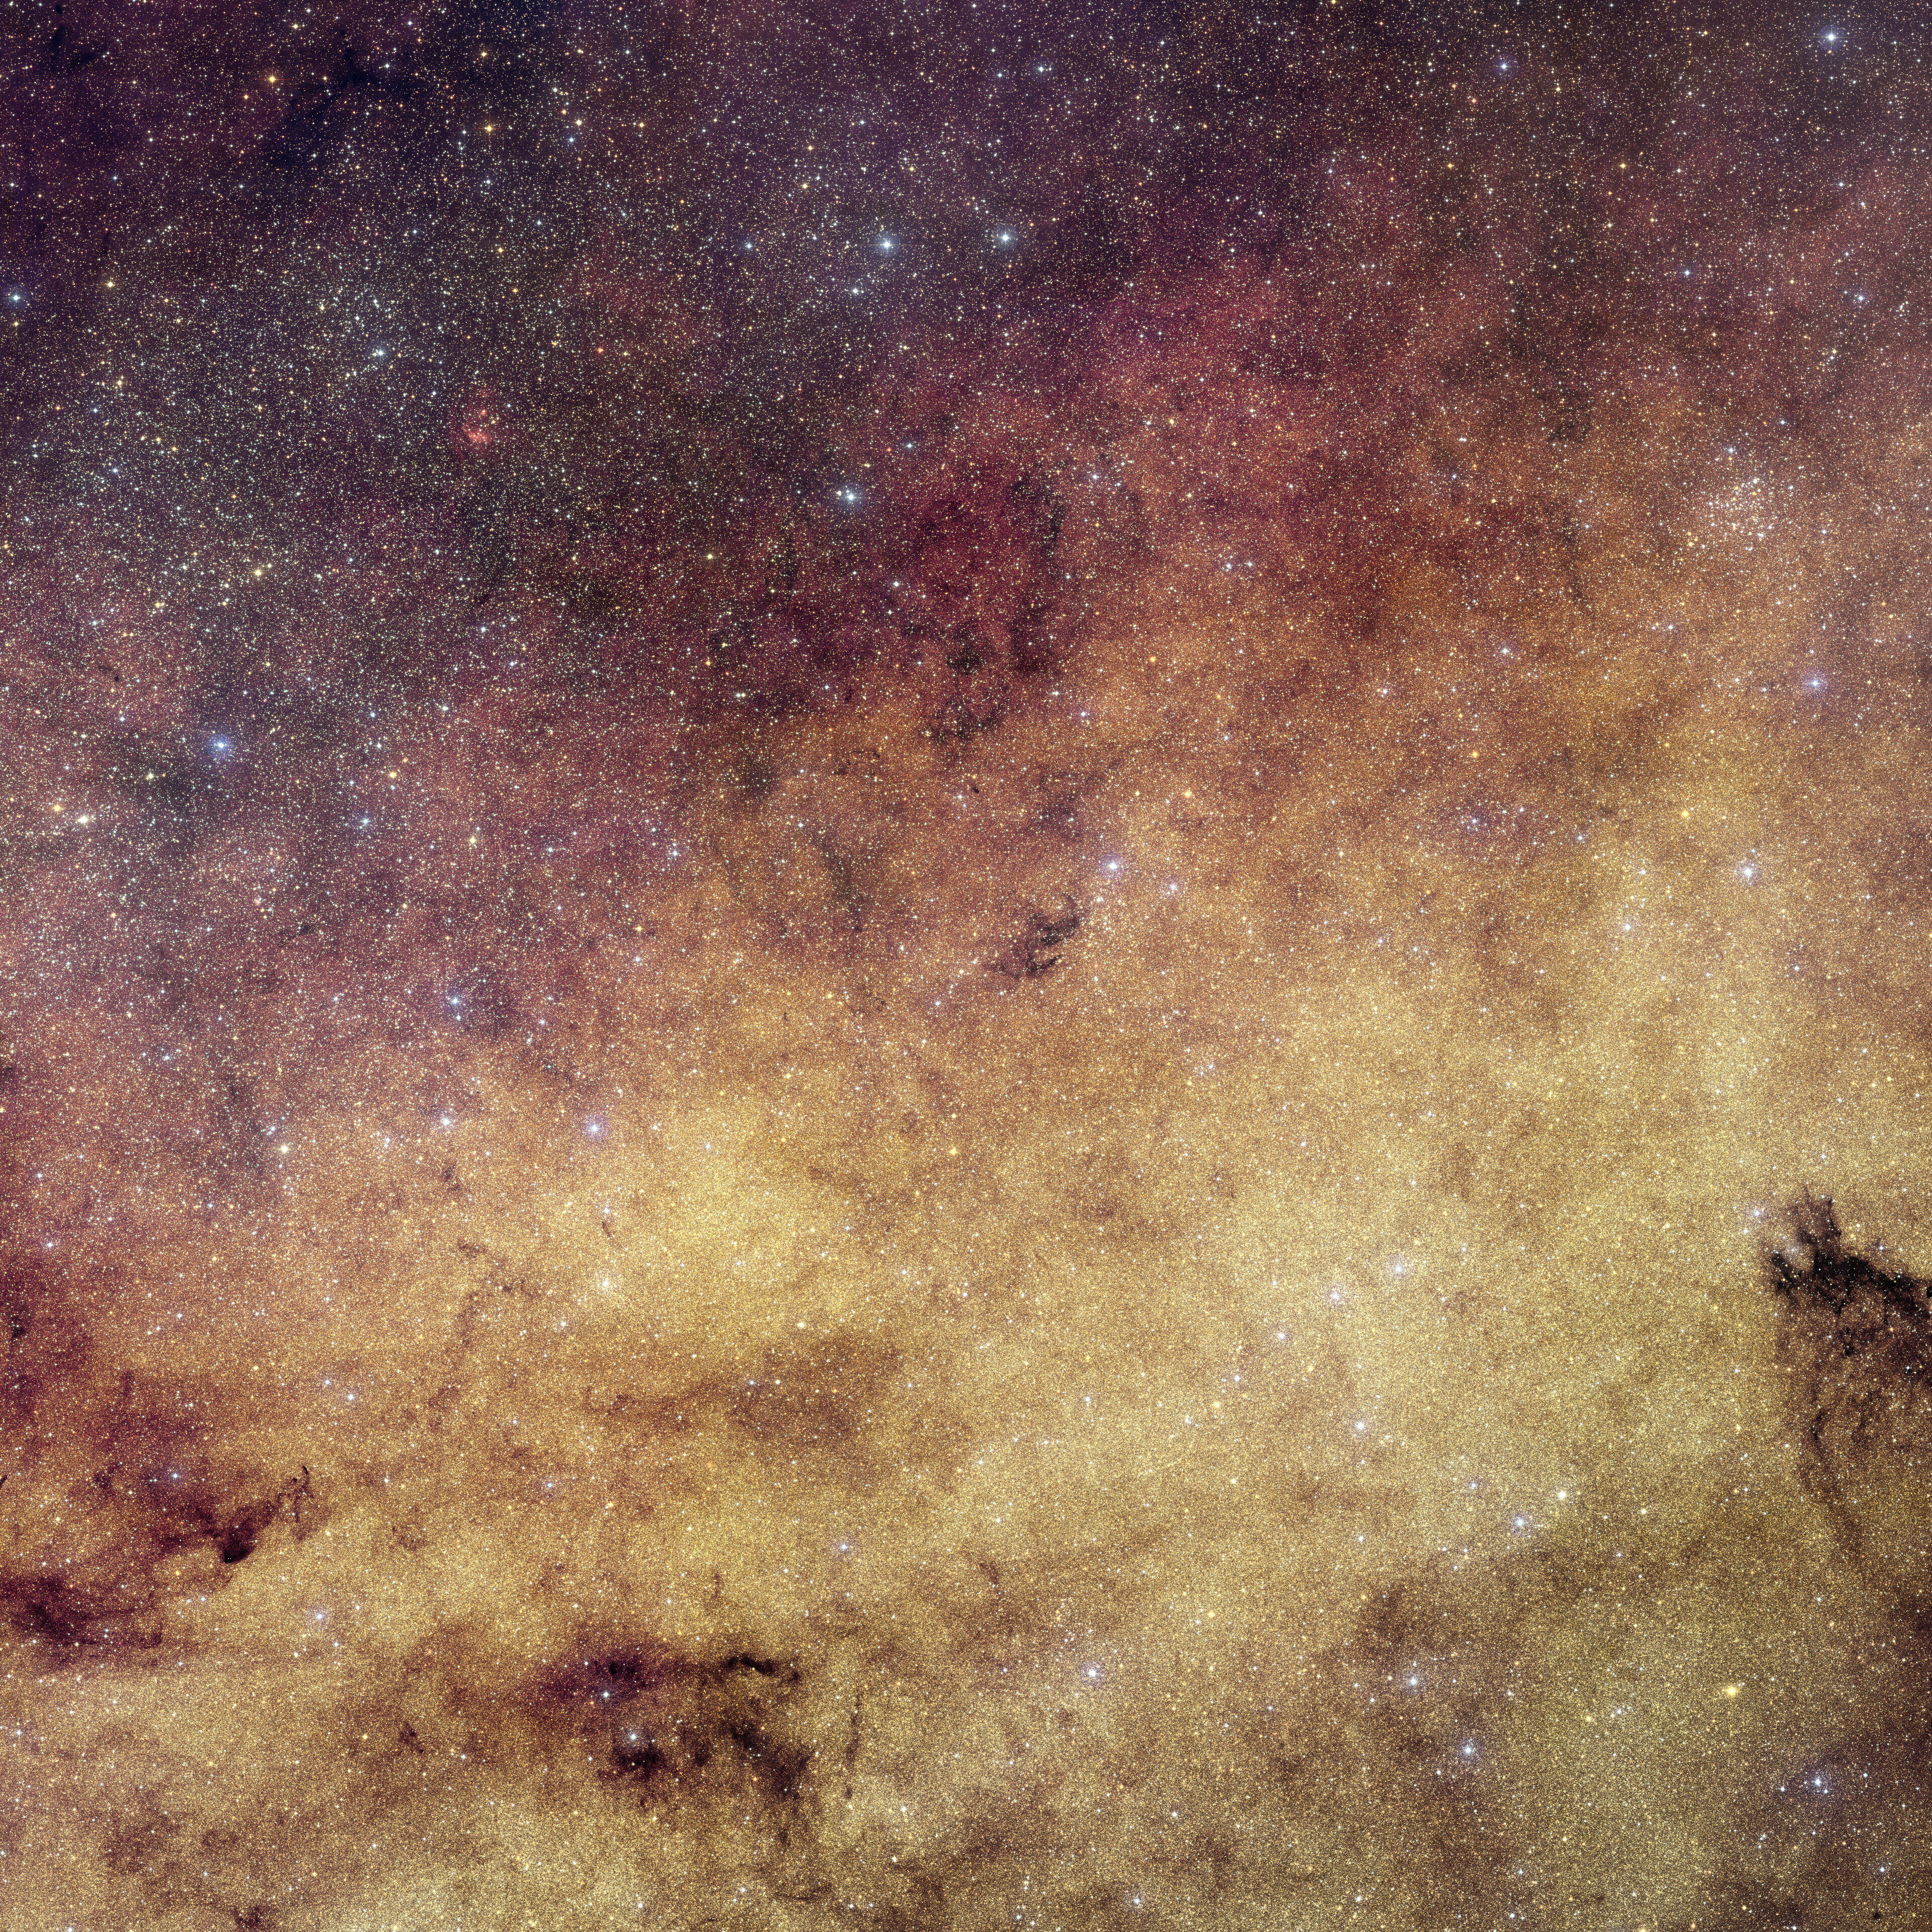
\includegraphics[width=\paperwidth]{euclid_bulge}};
  \node[bleedtitle, anchor=north west] at ([xshift=5mm, yshift=-4mm]current page.north west)
       {Black holes hide among these stars};
  \node[bleedtext, anchor=north west] at ([xshift=5mm, yshift=-15mm]current page.north west)
       {None of them shine};
  \bleedcredit{\href{https://www.nasa.gov/missions/roman-space-telescope/euclid-view-of-milky-way-heart-previews-core-survey-by-nasas-roman/}{ESA/Euclid/Euclid Consortium/NASA, CFHT; image processing J.-C.~Cuillandre \& E.~Bertin (CEA Paris-Saclay)}}
  \bleedsection
\end{tikzpicture}
\note{\begin{itemize}
  \item \emph{Euclid} with ground-based colour: a region near the Galactic centre that Roman's bulge survey will
        observe repeatedly.
  \item The Milky Way should hold $\sim10^8$ stellar black holes, and a field like this one hides many of them.
        Without a companion they emit nothing: the question of the next slides is how to find them.
\end{itemize}}
\end{frame}}


\begin{frame}{Almost every known black hole is in a binary}
\vspace{1mm}
$\sim\!10^8$ stellar black holes in the Milky Way; the known ones are seen through a \textbf{companion}\\
{\small (its light, X-rays from accretion, gravitational waves)}. \uncover<2->{Why not use those?}
\vspace{3mm}

\begin{columns}[T]
\begin{column}{.48\linewidth}
\textbf{In a binary}
\begin{itemize}\setlength{\itemsep}{5pt}
  \item<3-> \textbf{Mass} reshaped by the companion\\ {\small (mass transfer, stripped envelopes)}
  \item<4-> Only \textbf{weak kicks} survive\\ {\small (a strong kick unbinds the pair)}
  \item<5-> Seen only while \textbf{active}\\ {\small (X-ray outbursts: selection effects)}
\end{itemize}
\end{column}
\begin{column}{.48\linewidth}
\textbf{Isolated}
\begin{itemize}\setlength{\itemsep}{5pt}
  \item<3-> Mass set by the \textbf{star's own collapse}
  \item<4-> Carry their \textbf{full natal kick}
  \item<5-> Found by \textbf{gravity alone}:\\ every one can lens
\end{itemize}
\end{column}
\end{columns}
\vfill
\uncover<6->{%
\begin{beamercolorbox}[rounded=true,sep=6pt,wd=\linewidth]{block body alerted}
\centering
Binaries are not \emph{wrong}: they answer a different question (binary evolution).\\
Supernova physics and the Galaxy's black-hole census need the \textbf{isolated} ones too
\end{beamercolorbox}}
\vfill
\refnote{%
\ads{2020A\%26A...638A..94O}{Olejak et al.\ 2020};
\ads{2023MNRAS.518.1057E}{El-Badry et al.\ 2023};
\ads{2024A\%26A...686L...2G}{Gaia Collaboration 2024};
\ads{2012Sci...337..444S}{Sana et al.\ 2012, Science 337, 444};
\ads{2012MNRAS.425.2799R}{Repetto et al.\ 2012, MNRAS 425, 2799};
\ads{2012ApJ...757...36K}{Kreidberg et al.\ 2012, ApJ 757, 36}}
\note{\begin{itemize}
  \item Stars above $\sim20\,\Msun$ end as black holes. Population syntheses: $1.2\times10^8$ at $\sim14\,\Msun$
        (Olejak et al.\ 2020), $2.2\times10^8$ at $5$--$16\,\Msun$ (Lam et al.\ 2020).
  \item Known ones: X-ray binaries (accretion from a companion), \emph{Gaia} BH1--3 (a companion's orbit),
        gravitational-wave mergers (distant galaxies).
  \item Most massive stars are born in binaries that interact (Sana et al.\ 2012): the companion strips or feeds the
        progenitor, so a binary black hole's mass records binary evolution, not single-star collapse alone.
  \item Kicks: a black hole kicked hard enough leaves its companion and becomes isolated. Binaries keep the
        weak-kick ones, so their velocities underestimate the kicks (Repetto et al.\ 2012 infer kicks from where X-ray
        binaries sit in the Galaxy, an indirect route).
  \item X-ray binaries are found in outburst, and their masses rest on orbital modelling: the apparent
        $2$--$5\,\Msun$ gap may be partly a systematic (Kreidberg et al.\ 2012).
  \item So the binary sample is a biased subset for these questions. Isolated black holes are the missing, unbiased
        complement, and microlensing is the one way to weigh them.
\end{itemize}}
\end{frame}

\begin{frame}{Why the isolated population matters}
\vspace{2mm}
\begin{columns}[c]
\begin{column}{.45\linewidth}
\begin{itemize}\setlength{\itemsep}{8pt}
  \item<+-> \textbf{Mass function:} is there a mass gap?
  \item<+-> \textbf{Natal kicks:} how fast are they born?
  \item<+-> \textbf{Abundance} $F$: their share of\\ the stellar mass, $0.5$--$3\%$
  \item<+-> These need \textbf{many} masses, not one
\end{itemize}
\end{column}
\begin{column}{.52\linewidth}
\centering
% schematic mass axis (log scale): \massx gives 3.3 units per decade
\begin{tikzpicture}[x=1.05cm, y=1.1cm, font=\footnotesize]
  \fill[orange!45] ({\massx{1.1}},1.0) rectangle ({\massx{2.0}},1.45);
  \node[anchor=south, align=center, font=\scriptsize] at ({\massx{1.45}},1.45) {neutron\\ stars};
  \fill[pattern=north east lines, pattern color=jdgrey] ({\massx{2.0}},1.0) rectangle ({\massx{5.0}},1.45);
  \node[anchor=south, text=jdgrey] at ({\massx{3.2}},1.45) {gap?};
  \fill[jdblue!60] ({\massx{5}},1.0) rectangle ({\massx{20}},1.45);
  \node[anchor=south, align=center, font=\scriptsize] at ({\massx{12}},1.45) {X-ray\\ binaries};
  \fill[violet!35] ({\massx{5}},0.25) rectangle ({\massx{100}},0.7);
  \node[anchor=west] at ({\massx{20}},0.475) {GW mergers};
  \draw[-{Latex}] (0,0) -- (6.9,0);
  \foreach \m/\l in {1/1, 10/10, 100/100} \draw ({\massx{\m}},0) -- ({\massx{\m}},-0.12) node[below] {\l};
  \foreach \m in {2,3,4,5,6,7,8,9,20,30,40,50,60,70,80,90} \draw ({\massx{\m}},0) -- ({\massx{\m}},-0.06);
  \node[below] at (3.3,-0.45) {mass [$\Msun$]};
  \uncover<4->{
  \draw[red!70!black, thick] ({\massx{7.1}},-0.05) -- ({\massx{7.1}},2.2);
  \node[red!70!black, anchor=south, align=center] at ({\massx{7.1}},2.2) {one isolated BH\\ (OGLE-2011-BLG-0462)};
  \fill[jdgreen!25, rounded corners] (0.2,-1.55) rectangle (6.6,-0.95);
  \node at (3.4,-1.25) {isolated black holes: \textbf{?}};}
\end{tikzpicture}
\end{column}
\end{columns}
\vspace{3mm}
\uncover<5->{%
\begin{beamercolorbox}[rounded=true,sep=6pt,wd=\linewidth]{block body alerted}
\centering
Isolated black holes are dark: \textbf{gravitational microlensing} is the only way to \emph{see} and \emph{weigh} them
\end{beamercolorbox}}
\vfill
\refnote{%
\ads{2012ApJ...749...91F}{Fryer et al.\ 2012, ApJ 749, 91};
\ads{2022MNRAS.516.4971S}{Sweeney et al.\ 2022, MNRAS 516, 4971};
\ads{2020ApJ...889...31L}{Lam et al.\ 2020, ApJ 889, 31}}
\note{\begin{itemize}
  \item X-ray binary masses peak near $8\,\Msun$ with a deficit below $\sim5\,\Msun$: a real gap above the neutron
        stars, or a selection effect? The answer traces the supernova mechanism (rapid vs delayed, Fryer et al.\ 2012).
  \item Natal kicks: the velocities black holes receive at birth.
  \item An isolated black hole accretes too little from the interstellar medium to be seen. Microlensing needs no
        light from the lens, only its gravity.
  \item $F$ = the black holes' share of the Galaxy's stellar mass; the literature range is a factor $\sim6$.
\end{itemize}}
\end{frame}

% !TeX root = ../seminar.tex
\section{Gravitational Microlensing}

{\setbeamercolor{background canvas}{bg=black}
\begin{frame}[plain]
\begin{tikzpicture}[remember picture, overlay]
  \node[anchor=east, inner sep=0] at (current page.east)
       {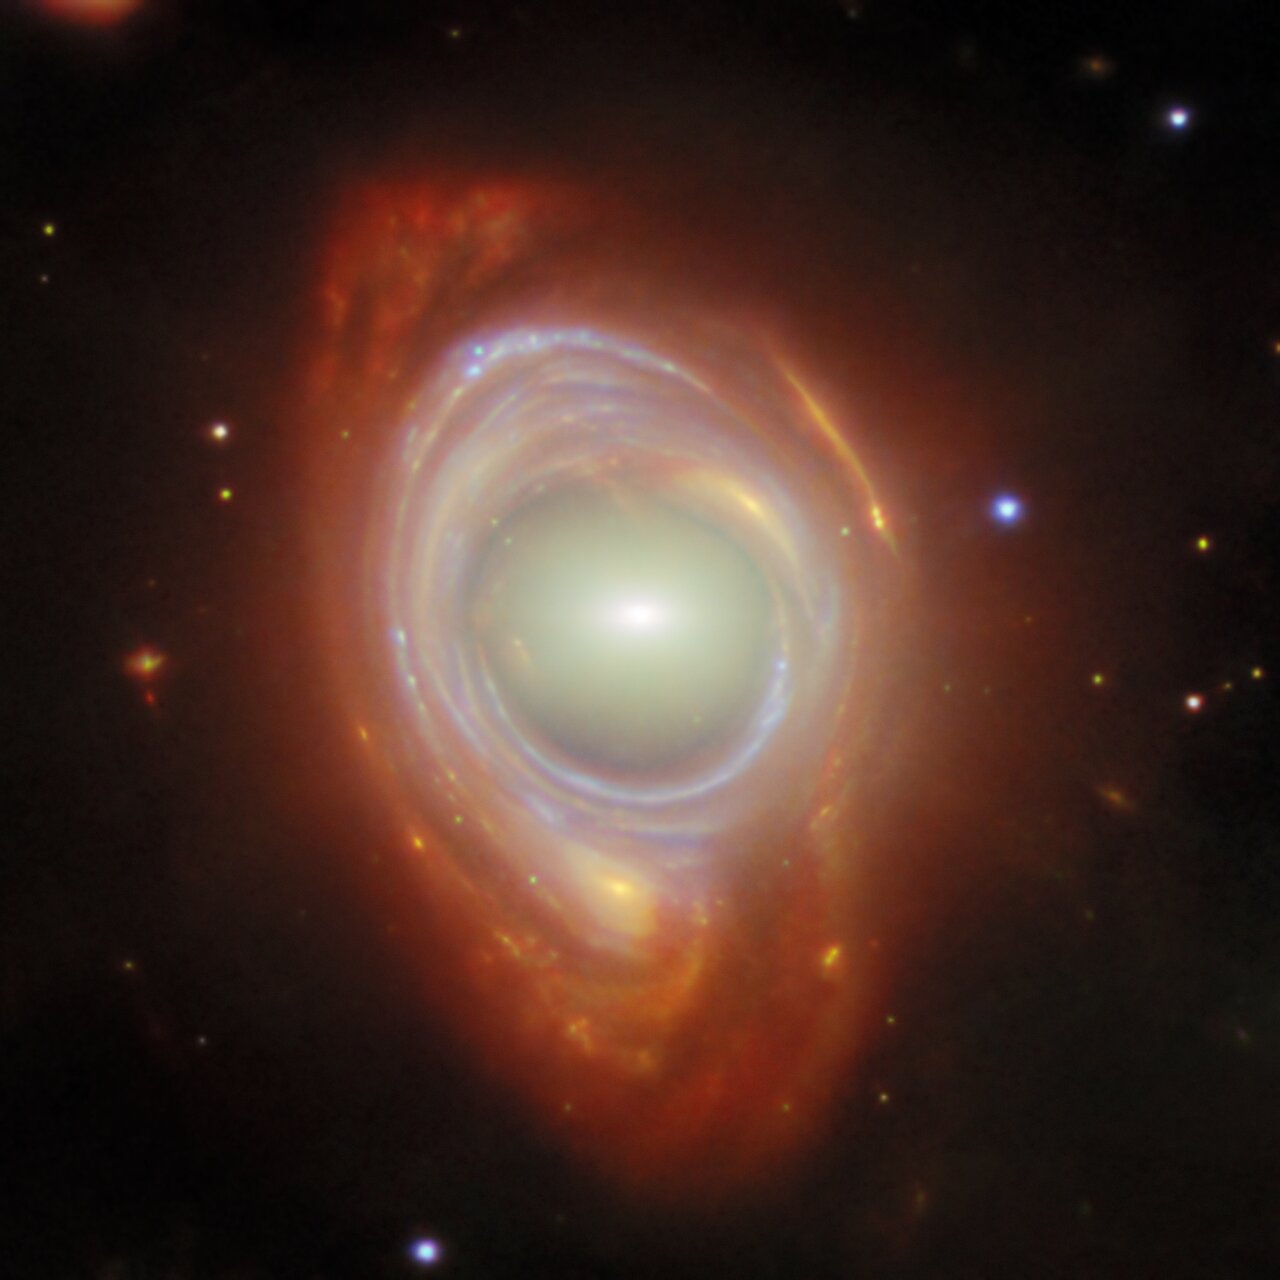
\includegraphics[height=\paperheight]{webb_einstein_ring}};
  \node[anchor=west, text=white, font=\huge\bfseries] at ([xshift=8mm, yshift=8mm]current page.west)
       {Gravity bends light};
  \node[anchor=north west, text=white, align=left, text width=6.2cm] at ([xshift=8mm, yshift=1mm]current page.west)
       {A galaxy \emph{behind} a galaxy,\\ stretched into a ring};
  \node[anchor=north west, text=white, align=left, text width=6.2cm] at ([xshift=8mm, yshift=-12mm]current page.west)
       {\small Our lenses are stars and black holes:\\ the ring is $\sim$\,mas, \textbf{too small to see}};
  \bleedcredit{\href{https://esawebb.org/images/potm2503a/}{ESA/Webb, NASA \& CSA, G.~Mahler (CC BY 4.0)}}
  \bleedsection
\end{tikzpicture}
\note{\begin{itemize}
  \item An Einstein ring imaged by \emph{JWST}: an elliptical galaxy in the cluster SMACSJ0028.2$-$7537 bends the light of a
        spiral far behind it into a near-complete ring.
  \item Galaxy lenses give rings of arcseconds; a star or a black hole gives $\tetE\sim0.5$--$5$\,mas. We do not see the
        ring: we see the star brighten and shift.
\end{itemize}}
\end{frame}}

\begin{frame}{A point lens: two images and the Einstein radius}
\centering
\vspace{1mm}
% Schematic, but the image angles obey the lens equation for beta = 0.06, theta_E = 0.25 (D_S = 10).
\begin{tikzpicture}[x=0.9cm, y=0.62cm, font=\footnotesize]
  \draw[jdlightgrey, dashed] (-0.3,0) -- (10.6,0);
  \draw[jdverylightgrey] (4.2,-2.5) -- (4.2,3.0) node[above, text=jdgrey] {lens plane};
  \draw[jdverylightgrey] (10,-2.5) -- (10,3.0) node[above, text=jdgrey] {source plane};
  % observer, lens, source
  \fill (0,0) circle (2pt) node[below=2pt] {observer};
  \fill[black] (4.2,0) circle (3.5pt);
  \node[below=6pt, fill=white, inner sep=1pt] at (4.2,0) {lens $M$};
  \node[star, star points=5, star point ratio=2.2, fill=yellow!80!orange, draw=orange!70!black,
        inner sep=1.6pt] (S) at (10,0.6) {};
  \node[right=2pt] at (S) {source};
  % the two light paths
  \draw[orange!80!black, thick, -{Latex[length=2mm]}] (10,0.6) -- (4.2,1.184) -- (0,0);
  \draw[orange!80!black, thick, -{Latex[length=2mm]}] (10,0.6) -- (4.2,-0.932) -- (0,0);
  % where the observer sees the images
  \uncover<2->{
  \draw[orange!80!black, dotted, thick] (0,0) -- (10,0.6);
  \draw[jdblue, densely dashed] (4.2,1.184) -- (10,2.818);
  \draw[jdblue, densely dashed] (4.2,-0.932) -- (10,-2.218);
  \node[star, star points=5, star point ratio=2.2, fill=yellow!40, draw=orange!50, inner sep=1.3pt]
       at (10,2.818) {};
  \node[star, star points=5, star point ratio=2.2, fill=yellow!40, draw=orange!50, inner sep=0.9pt]
       at (10,-2.218) {};
  \node[right=3pt, text=jdblue] at (10,2.818) {image $+$};
  \node[right=3pt, text=jdblue] at (10,-2.218) {image $-$};
  % angles at the observer
  \draw[jdblue] (1.6,0) arc (0:15.8:1.6);
  \node[text=jdblue] at (1.95,0.27) {$\theta$};
  \draw[orange!80!black] (2.8,0) arc (0:3.4:2.8);
  \node[text=orange!80!black] at (3.12,0.1) {$\beta$};}
  % distances
  \draw[{Latex[length=1.6mm]}-{Latex[length=1.6mm]}] (0,-2.0) -- node[fill=white, inner sep=1pt] {$D_L$} (4.2,-2.0);
  \draw[{Latex[length=1.6mm]}-{Latex[length=1.6mm]}] (0,-2.55) -- node[fill=white, inner sep=1pt] {$D_S$} (10,-2.55);
\end{tikzpicture}

\vspace{3mm}
\uncover<3->{%
\[
  \beta = \theta - \frac{\tetE^2}{\theta}
  \qquad\qquad
  \tetE = \sqrt{\kappa\,M\,\pirel}
\]
{\small\color{jdgrey} $\kappa = 8.14$\,mas$/\Msun$, \quad $\pirel = {\rm AU}\,(1/D_L - 1/D_S)$: the lens--source parallax}\par}
\vspace{1mm}
\uncover<4->{bulge star: $\tetE\approx0.4$\,mas \qquad black hole: $\tetE\approx5$\,mas, images $\gtrsim10$\,mas apart}
\vfill
\refnote{\ads{1986ApJ...304....1P}{Paczy\'nski 1986, ApJ 304, 1}}
\note{\begin{itemize}
  \item Images at $\theta_\pm = \tfrac{\tetE}{2}\bigl(u\pm\sqrt{u^2+4}\bigr)$, $u=\beta/\tetE$.
  \item $\kappa = 8.144\,{\rm mas}/\Msun$, $\pirel = {\rm AU}(1/D_L-1/D_S)$.
  \item Bulge star: $0.5\,\Msun$, $D_L=6$, $D_S=8$\,kpc. Black hole: $10\,\Msun$ at $2$\,kpc.
  \item The two images are $\sim2\tetE$ apart: usually far too close to separate.
\end{itemize}}
\end{frame}

\begin{frame}{A lens crossing a star}
\centering
\vspace{2mm}
\animategraphics[autoplay, loop, controls=off, poster=40, width=.76\linewidth]{16}{img/anim/frame_}{00}{80}

\vspace{4mm}
We see only the \textbf{total light} (top: \textbf{photometry})\\ and where its \textbf{centre} lies (bottom: \textbf{astrometry})
\vfill
\refnote{Reverse ray tracing of a limb-darkened star, $R_\star=0.6\,\tetE$ (A.~Salehi); the curves are
measured from the traced images.}
\note{\begin{itemize}
  \item In a real event the images are too close to separate: a telescope sees only their total light and its centre.
  \item Near the peak the lens is \emph{inside} the stellar disc: an Einstein ring forms, the finite source caps the
        magnification and reverses the centroid shift. Dashed grey: a point source.
\end{itemize}}
\end{frame}

\begin{frame}{Two observables: photometry and astrometry}
\vspace{1mm}
\centering
The two images are $\sim2\tetE$ apart: usually unresolved, seen as one blended star
\vspace{1mm}
\begin{columns}[T]
\begin{column}{.47\linewidth}
\centering
\textbf{Photometry}: \emph{how bright?}\\
{\small the star's flux vs.\ time (the light curve)}
\[
  A(u) = \frac{u^2+2}{u\sqrt{u^2+4}}
\]
\uncover<2->{%
\[
  \tE = \frac{\tetE}{\mu_{\rm rel}}
\]
mixes \textbf{mass}, \textbf{distance}, \textbf{velocity}}
\end{column}
\begin{column}{.47\linewidth}
\centering
\uncover<3->{%
\textbf{Astrometry}: \emph{where?}\\
{\small the light centre's position on the sky vs.\ time}
\[
  \delta\theta = \frac{\tetE\,u}{u^2+2}
\]
\[
  \delta\theta_{\max} = \frac{\tetE}{\sqrt8}\quad\text{at } u=\sqrt2
\]
measures $\tetE$ directly}
\end{column}
\end{columns}
\vfill
{\centering\small\color{jdgrey} $u$: lens--source separation in units of $\tetE$; \quad $\mu_{\rm rel}$: their relative proper motion\par}
\vspace{1mm}
\refnote{\ads{1986ApJ...304....1P}{Paczy\'nski 1986, ApJ 304, 1};
\ads{2000ApJ...542..785G}{Gould 2000, ApJ 542, 785}}
\note{\begin{itemize}
  \item $u(t) = \sqrt{u_0^2 + ((t-t_0)/\tE)^2}$: impact parameter $u_0$, peak time $t_0$.
  \item The timescale is the one physical quantity a simple light curve gives. Bulge events: $\tE\sim20$\,d;
        black holes: hundreds of days.
  \item The centroid shift peaks $\sim1.4\,\tE$ from the photometric peak, often in a different Roman season.
  \item The images are $\Delta\theta=\tetE\sqrt{u^2+4}\ge2\tetE$ apart: $\gtrsim10$\,mas for tens of $\Msun$ at a few kpc,
        so for heavy, nearby lenses they may be resolved.
\end{itemize}}
\end{frame}

\begin{frame}{Microlensing parallax: a second viewpoint}
\vspace{1mm}
\centering
\begin{tikzpicture}[font=\footnotesize, x=1cm, y=1cm]
  % left: annual parallax (Earth's orbit makes the track wiggle)
  \begin{scope}
    \draw[jdlightgrey, fill=jdverylightgrey!40] (0,0) circle (1.1);
    \fill (0,0) circle (2pt) node[below left=-1pt] {lens};
    \node[text=jdgrey, font=\scriptsize] at (0,1.35) {Einstein ring};
    \draw[orange!80!black, dashed, -{Latex}] (-2.3,0.35) -- (2.3,0.35);
    \uncover<2->{\draw[orange!80!black, very thick, -{Latex}, domain=-2.3:2.3, samples=80]
         plot (\x, {0.35+0.28*sin(deg(2.6*\x))});
    \node[align=center, font=\small] at (0,-1.85) {\textbf{annual}: Earth's orbit\\ \footnotesize needs a long event};}
  \end{scope}
  % right: satellite parallax (Earth and L2 see different tracks)
  \uncover<3->{
  \begin{scope}[xshift=6.0cm]
    \draw[jdlightgrey, fill=jdverylightgrey!40] (0,0) circle (1.1);
    \fill (0,0) circle (2pt);
    \draw[jdblue, very thick, -{Latex}] (-2.3,0.25) -- (2.3,0.25) node[right] {Earth};
    \draw[red!70!black, very thick, -{Latex}] (-2.3,0.65) -- (2.3,0.65) node[right] {L2};
    \draw[{Latex[length=1.3mm]}-{Latex[length=1.3mm]}] (-1.75,0.25) -- node[left=1pt] {$\Delta u$} (-1.75,0.65);
    \node[align=center, font=\small] at (0,-1.85) {\textbf{satellite}: Roman vs.\ Rubin\\ \footnotesize works for short events too};
  \end{scope}}
\end{tikzpicture}

\vspace{1mm}
\[
  \piE = \frac{\pirel}{\tetE}
  \qquad
  \uncover<2->{\vec u(t) = \vec u_0 + \frac{t-t_0}{\tE}\,\hat{\vec\mu} + \piE\,\vec s(t)}
  \qquad
  \uncover<3->{\Delta u \simeq \piE\,\frac{D_\perp}{\rm AU}}
\]
\uncover<4->{Black hole: $\piE=\sqrt{\pirel/\kappa\Ml}$ is \textbf{small} $\Rightarrow$ a small, slow wiggle}
\vfill
\refnote{\ads{1966MNRAS.134..315R}{Refsdal 1966, MNRAS 134, 315};
\ads{1992ApJ...392..442G}{Gould 1992, ApJ 392, 442};
\ads{2000ApJ...542..785G}{Gould 2000, ApJ 542, 785}}
\note{\begin{itemize}
  \item Parallax: the same lens--source pair seen from a different place lines up differently. $\piE$ is the relative
        parallax $\pirel={\rm AU}(1/D_L-1/D_S)$ in units of $\tetE$: one AU of observer motion moves the track by
        $\piE$ Einstein radii.
  \item Annual: $\vec s(t)$ = Earth's (or Roman's) displacement from uniform motion, in AU, projected on the sky.
        It needs $\tE$ to be a sizeable fraction of a year: black holes qualify.
  \item Satellite: two observers $D_\perp$ apart see the peak at different times and heights, at the same moment,
        so it needs no long event (as with \emph{Spitzer}). Roman (L2) and Earth: $D_\perp\approx0.01$\,AU, so
        $\Delta u\approx0.01\,\piE$.
  \item The expectation going in: Roman + Rubin give a satellite parallax. The results test it.
  \item Black hole, $10\,\Msun$ at $2$\,kpc, source at $8$\,kpc: $\piE\approx0.05$.
\end{itemize}}
\end{frame}

\begin{frame}{From observables to a lens mass}
\centering
\vspace{2mm}
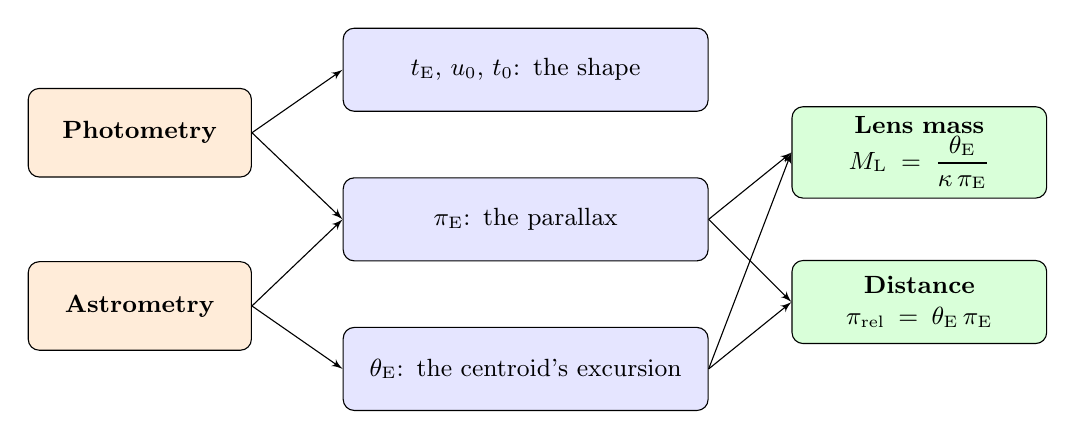
\begin{tikzpicture}[font=\small,
    ob/.style={terminator, fill=orange!15, text width=2.6cm, align=center, minimum height=3.2em},
    qu/.style={terminator, fill=blue!10, text width=4.4cm, align=center, minimum height=3em},
    re/.style={terminator, fill=green!15, text width=3.0cm, align=center, minimum height=3em}]
  \node[ob] (ph) at (0,1.1) {\textbf{Photometry}};
  \node[ob] (as) at (0,-1.1) {\textbf{Astrometry}};
  \node[qu] (te) at (4.9,1.9) {$\tE$, $u_0$, $t_0$: the shape};
  \uncover<2->{\node[qu] (pi) at (4.9,0) {$\piE$: the parallax};}
  \uncover<3->{\node[qu] (th) at (4.9,-1.9) {$\tetE$: the centroid's excursion};}
  \uncover<4->{
  \node[re] (m) at (9.9,0.85) {\textbf{Lens mass}\\ $\Ml = \dfrac{\tetE}{\kappa\,\piE}$};
  \node[re] (d) at (9.9,-1.05) {\textbf{Distance}\\ $\pirel = \tetE\,\piE$};}
  \path[connector] (ph.east) -- (te.west);
  \uncover<2->{\path[connector] (ph.east) -- (pi.west); \path[connector] (as.east) -- (pi.west);}
  \uncover<3->{\path[connector] (as.east) -- (th.west);}
  \uncover<4->{
  \path[connector] (pi.east) -- (m.west); \path[connector] (th.east) -- (m.west);
  \path[connector] (pi.east) -- (d.west); \path[connector] (th.east) -- (d.west);}
\end{tikzpicture}

\vspace{5mm}
\uncover<5->{%
\[
  \left(\frac{\sigma_M}{M}\right)^2 = \left(\frac{\sigma_{\piE}}{\piE}\right)^2 + \left(\frac{\sigma_{\tetE}}{\tetE}\right)^2
\]
Black holes: $\tetE$ large (easy), $\piE$ small (hard)}
\vfill
\refnote{\ads{2000ApJ...542..785G}{Gould 2000, ApJ 542, 785}}
\note{\begin{itemize}
  \item $\piE = \pirel/\tetE$: from the light curve's distortion by Earth's orbit (annual parallax), or from two
        observers at once (satellite parallax: Roman at L2, Rubin on Earth, $0.01$\,AU apart).
  \item $\tetE$: from the size of the centroid's excursion, or from the separation of the two images.
\end{itemize}}
\end{frame}

{\setbeamercolor{background canvas}{bg=black}
\begin{frame}[plain]
\begin{tikzpicture}[remember picture, overlay]
  \node[anchor=north, inner sep=0] (im) at (current page.north)
       {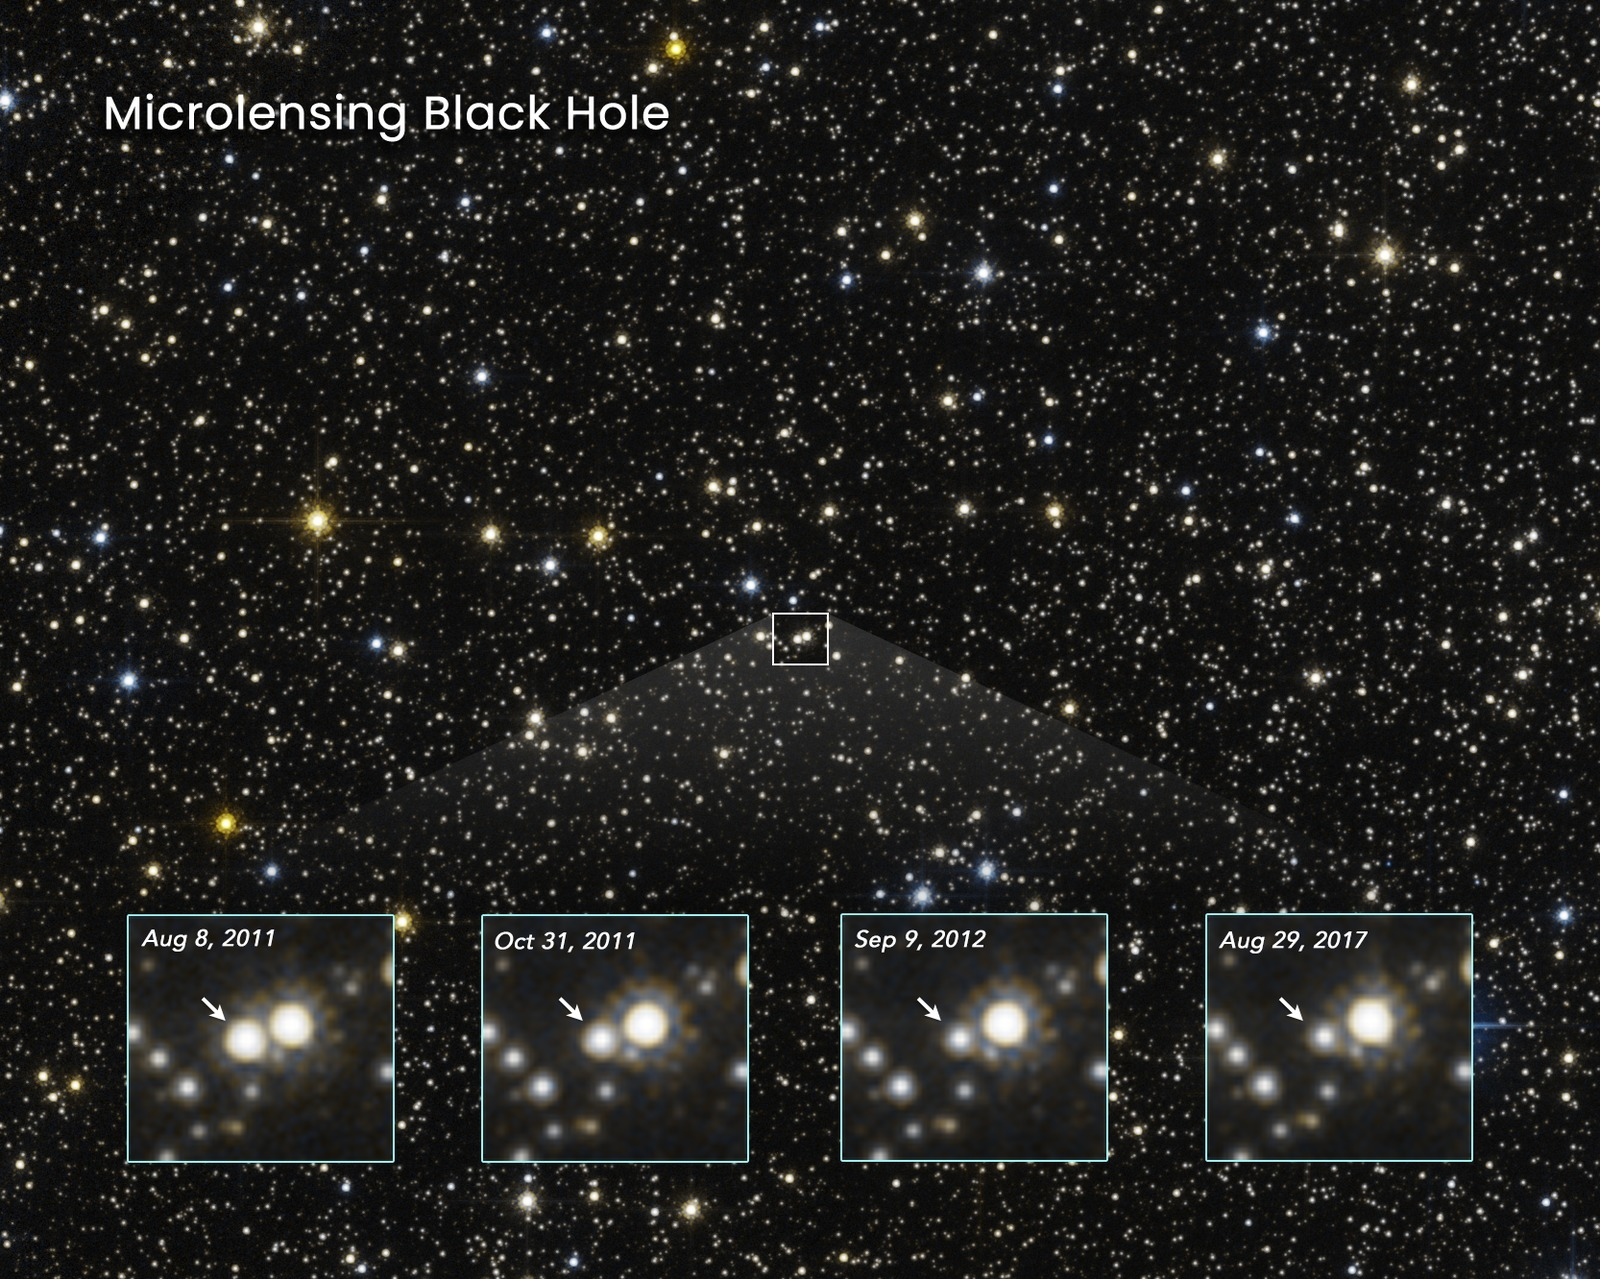
\includegraphics[height=.88\paperheight]{stsci_isolated_bh}};
  \node[anchor=north, text=white, font=\normalsize] at ([yshift=-1mm]im.south)
       {2011--2017: \emph{Hubble} watches a star brighten and fade, lensed by \textbf{something unseen}};
  \bleedcredit{\href{https://www.astropix.org/image/stsci/2022-01b}{NASA, ESA, K.~Sahu (STScI)}}
\end{tikzpicture}
\note{\begin{itemize}
  \item Real \emph{HST} (WFC3/UVIS) data: a field toward the Galactic centre, and the source star of OGLE-2011-BLG-0462
        (arrow) in four epochs, bright in August 2011 and back to normal by 2017.
  \item The astrometric shift, $\sim1$\,mas, is a fraction of a pixel: not visible here, but measured from the
        star's position at each epoch.
  \item No light from the lens: an isolated, dark, compact object.
\end{itemize}}
\end{frame}}

\begin{frame}{The first isolated black hole: OGLE-2011-BLG-0462}
\vspace{1mm}
\begin{columns}[T]
\begin{column}{.38\linewidth}
\centering
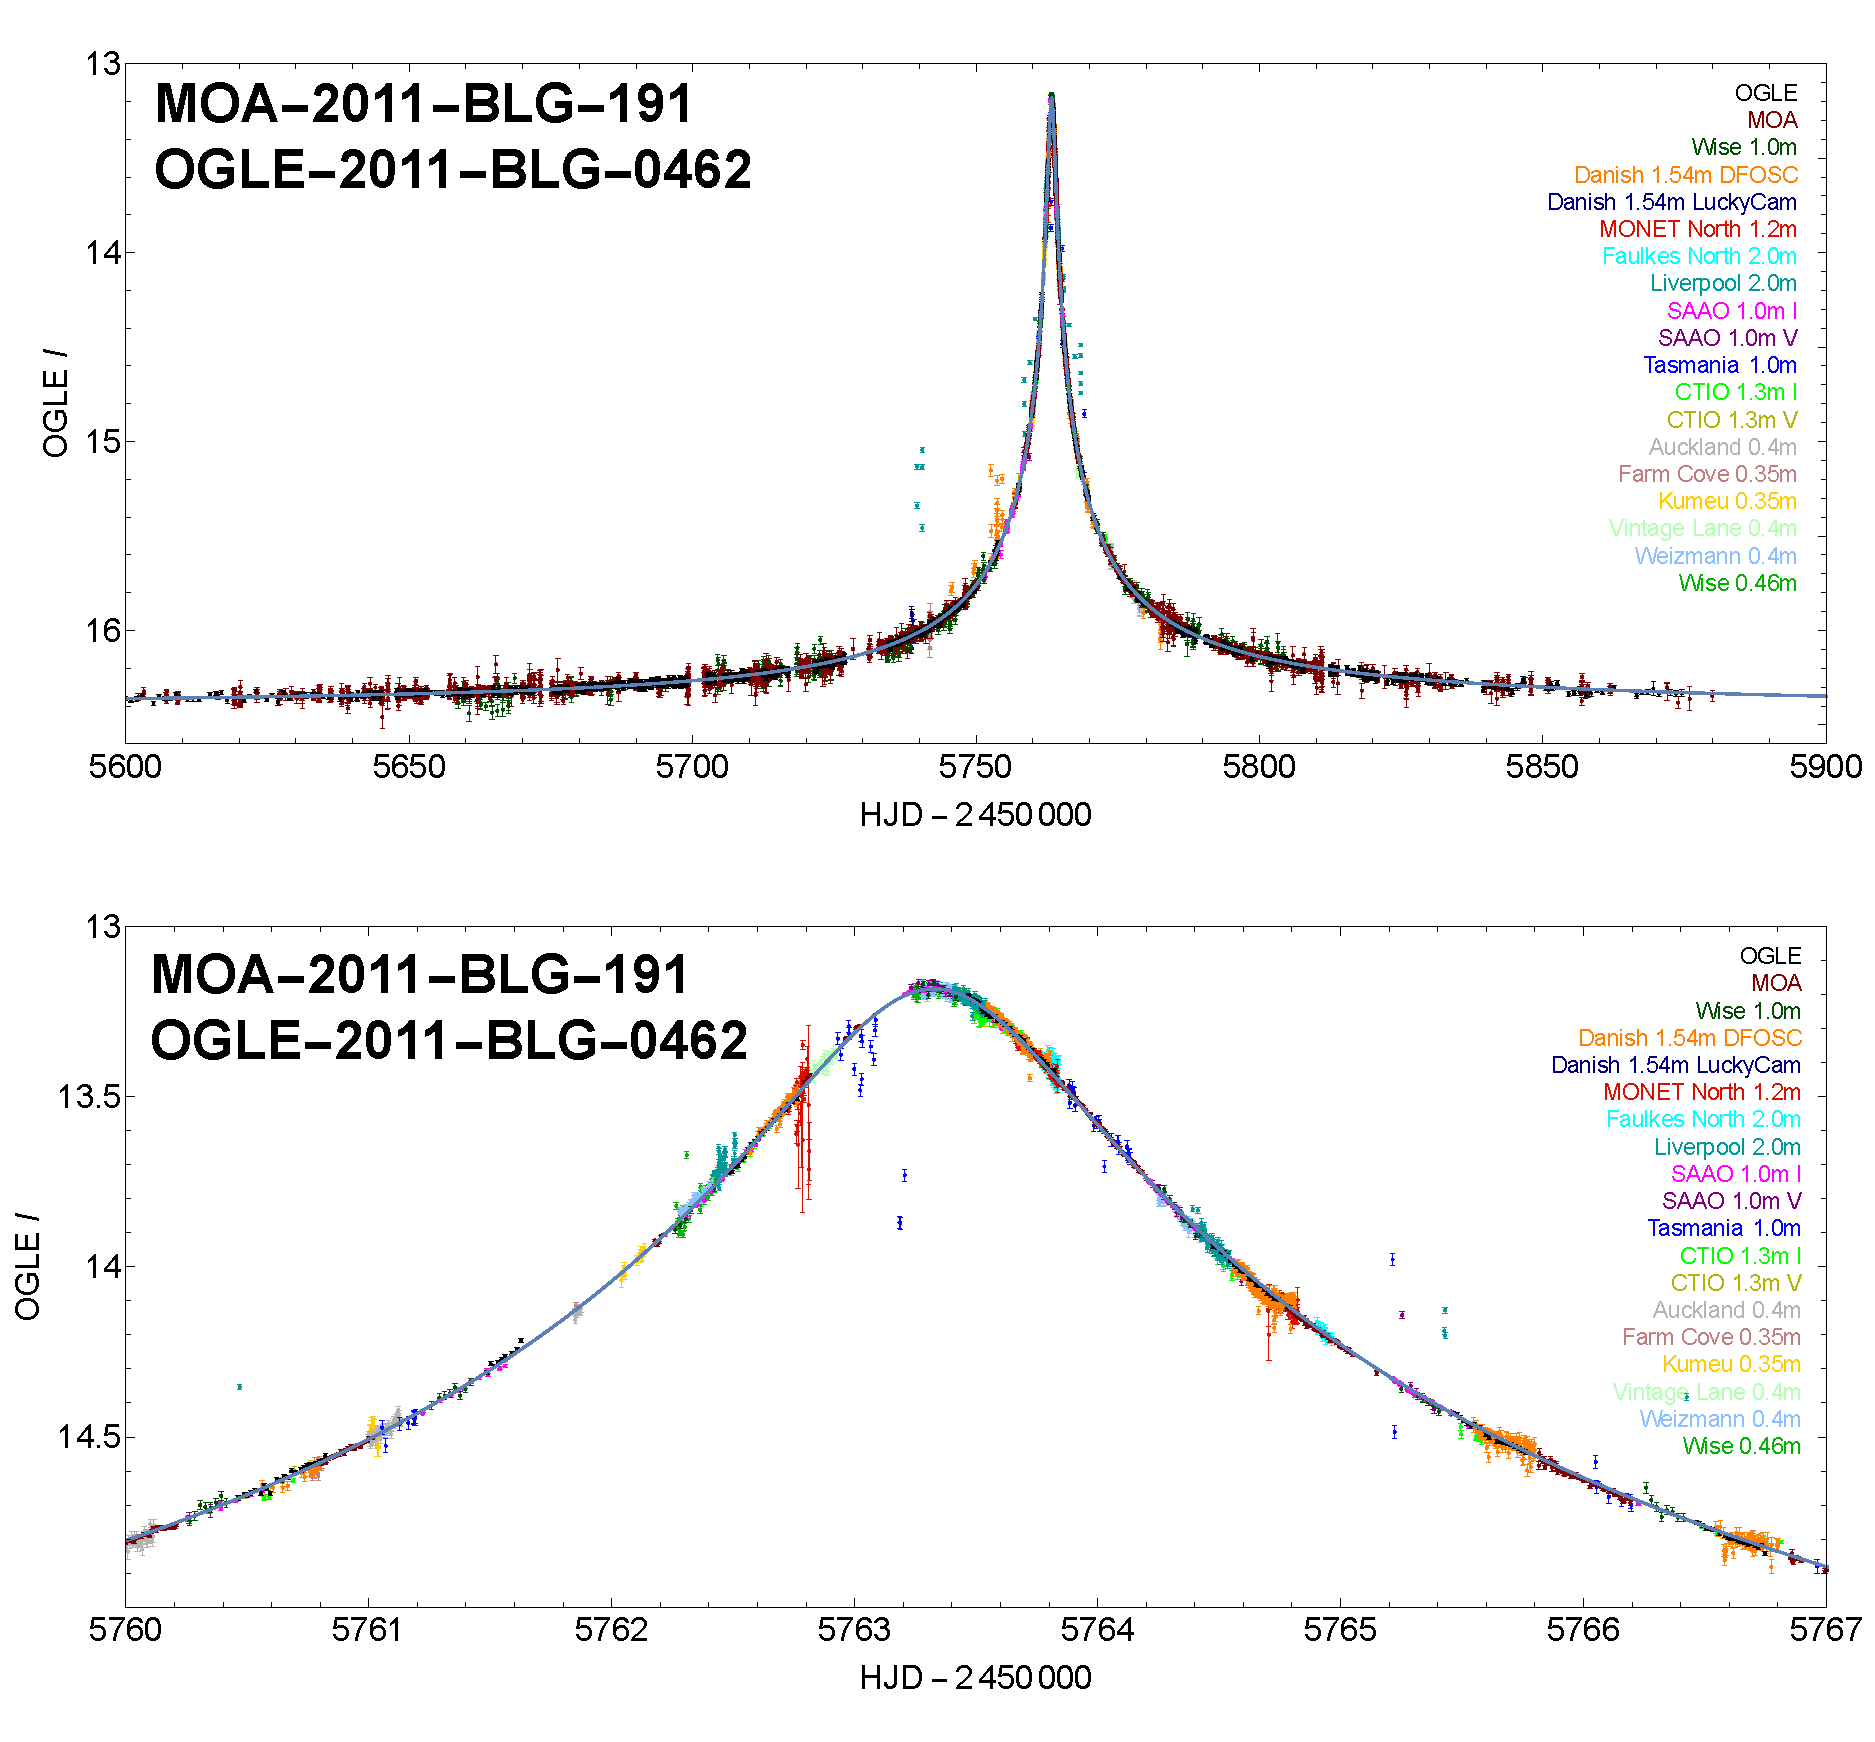
\includegraphics[width=.92\linewidth]{sahu2022_photometry}
\end{column}
\begin{column}{.24\linewidth}
\centering
\vspace{2mm}
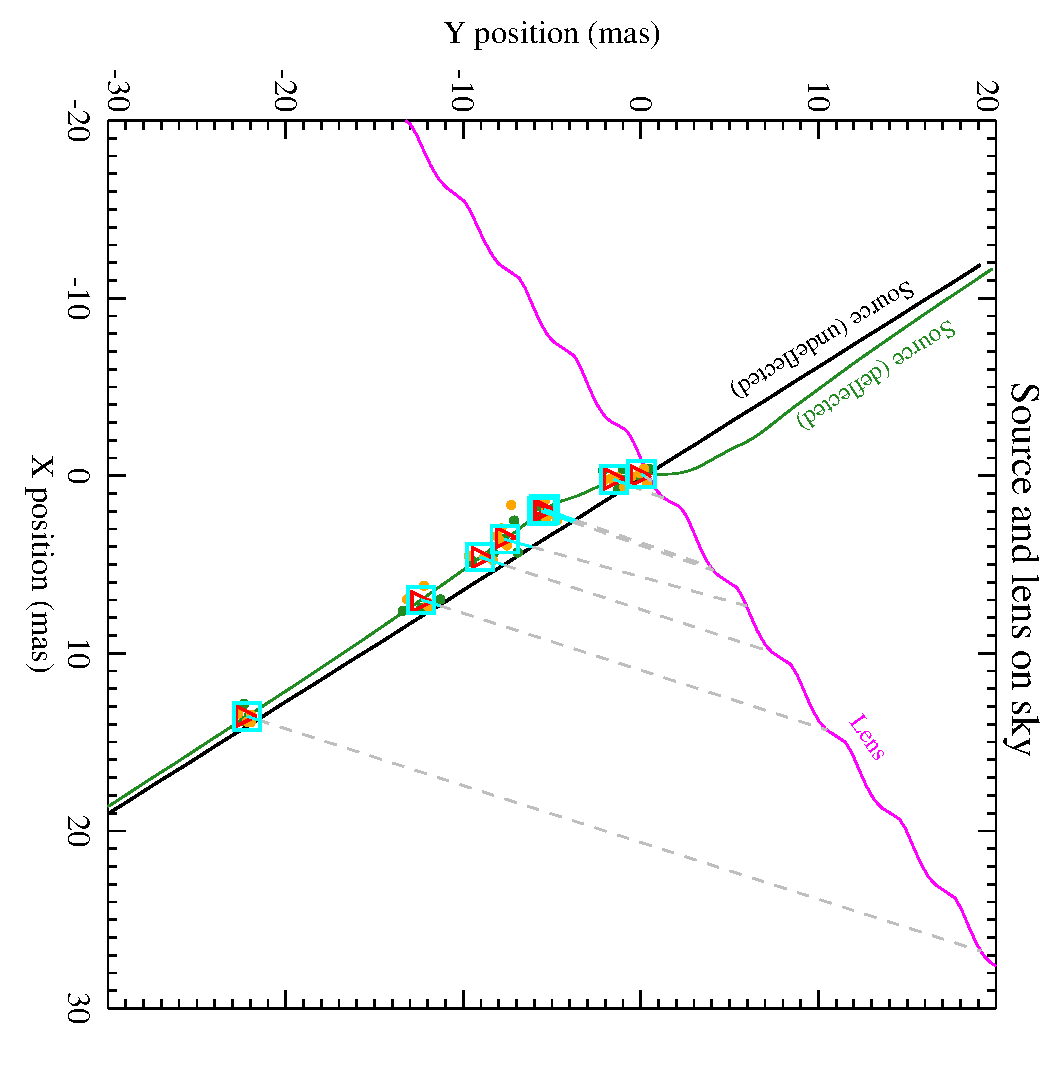
\includegraphics[angle=90,width=.9\linewidth]{sahu2022_sky}
\end{column}
\begin{column}{.34\linewidth}
\begin{itemize}\setlength{\itemsep}{6pt}
  \item<+-> Photometry: $\tE\approx270$\,d,\\ $\piE$ from the ground
  \item<+-> Astrometry: \emph{HST}, 6 years\\ $\to\tetE\approx5$\,mas
  \item<+-> $\Ml = 7.1\pm1.3\,\Msun$\\ at $1.6$\,kpc
\end{itemize}
\end{column}
\end{columns}
\vspace{2mm}
\credit{\ads{2022ApJ...933...83S}{Sahu et al.\ 2022, ApJ 933, 83}}
\vfill
\uncover<4->{%
\begin{beamercolorbox}[rounded=true,sep=6pt,wd=\linewidth]{block body alerted}
\centering
The first \textbf{dark} object weighed by its gravity alone:\\
both observables together \textbf{work}
\end{beamercolorbox}}
\vfill
\note{\begin{itemize}
  \item Sahu et al.\ 2022: a decade-long \emph{HST} programme following up long ground-based events.
  \item Left: the light curve (OGLE, MOA, \ldots) and its parallax distortion. Right: the source's measured
        position over 6 years, deflected by $\sim1$\,mas.
  \item $\tetE\approx5.2$\,mas and $\piE\approx0.09$: $\Ml = \tetE/(\kappa\piE)\approx7\,\Msun$, no light from the lens
        $\to$ a black hole. Isolated: no companion in the data.
  \item Its transverse velocity ($\sim45$\,km/s relative to the disc) hints at a natal kick.
\end{itemize}}
\end{frame}

\begin{frame}{\ldots but how heavy is it?}
\vspace{1mm}
\begin{columns}[c]
\begin{column}{.50\linewidth}
\centering
% published masses of the lens, linear axis 0-10 Msun, 0.6 cm per Msun
\begin{tikzpicture}[x=0.5cm, y=0.62cm, font=\footnotesize]
  \fill[orange!25] (1.1,-0.4) rectangle (2.3,4.6);
  \node[anchor=south, align=center, font=\scriptsize] at (1.7,4.6) {neutron\\ stars};
  \fill[jdblue!12] (5,-0.4) rectangle (10,4.6);
  \node[anchor=south, font=\scriptsize] at (7.5,4.6) {black holes};
  \draw[-{Latex}] (0,-0.4) -- (10.3,-0.4);
  \foreach \m in {0,2,...,10} \draw (\m,-0.4) -- (\m,-0.55) node[below] {\m};
  \node[below] at (5,-1.05) {lens mass [$\Msun$]};
  {\draw[jdblue!80!black, very thick, {|-|}] (5.8,3.9) -- (8.4,3.9); \fill[jdblue!80!black] (7.1,3.9) circle (2.5pt);
    \node[anchor=east, font=\tiny] at (-0.2,3.9) {Sahu+ 2022};}
  \uncover<2->{\draw[red!70!black, very thick, {|-|}] (1.6,2.8) -- (4.4,2.8);
    \node[anchor=east, font=\tiny] at (-0.2,2.8) {Lam+ 2022};}
  \uncover<4->{\draw[jdblue!80!black, very thick, {|-|}] (7.06,1.5) -- (8.70,1.5); \fill[jdblue!80!black] (7.88,1.5) circle (2.5pt);
    \node[anchor=east, font=\tiny] at (-0.2,1.5) {Mr\'oz+ 2022};
    \draw[jdblue!80!black, very thick, {|-|}] (4.98,0.4) -- (7.22,0.4); \fill[jdblue!80!black] (6.03,0.4) circle (2.5pt);
    \node[anchor=east, font=\tiny] at (-0.2,0.4) {Lam \& Lu 2023};}
\end{tikzpicture}
\end{column}
\begin{column}{.46\linewidth}
\begin{itemize}\setlength{\itemsep}{6pt}
  \item<2-> Same event, nearly the same data:\\ black hole \emph{or} neutron star?
  \item<3-> \textbf{Systematics}, not noise:\\ in $\piE$ (ground) and $\tetE$ (\emph{HST})
  \item<4-> Settled only by re-analysis:\\ a $\sim7\,\Msun$ black hole
\end{itemize}
\end{column}
\end{columns}
\vfill
\uncover<5->{%
\begin{beamercolorbox}[rounded=true,sep=6pt,wd=\linewidth]{block body alerted}
\centering
$\Ml=\tetE/\kappa\piE$: a bias in \emph{either} observable goes straight into the mass.\\
For a black hole $\piE$ is small and easily biased $\Rightarrow$ measure it robustly
\end{beamercolorbox}}
\vfill
\refnote{%
\ads{2022ApJ...933...83S}{Sahu et al.\ 2022, ApJ 933, 83};
\ads{2022ApJ...933L..23L}{Lam et al.\ 2022, ApJL 933, L23};
\ads{2022ApJ...937L..24M}{Mr\'oz, Udalski \& Gould 2022, ApJL 937, L24};
\ads{2023ApJ...955..116L}{Lam \& Lu 2023, ApJ 955, 116}}
\note{\begin{itemize}
  \item Lam et al.\ 2022 analysed similar photometry and \emph{HST} astrometry and found $1.6$--$4.4\,\Msun$: a neutron
        star could not be excluded.
  \item The difference lay in the systematics: the ground-based parallax (which data sets, how their errors are
        treated) and the reduction of the \emph{HST} images.
  \item Mr\'oz, Udalski \& Gould 2022 re-derived the parallax from OGLE photometry; Lam \& Lu 2023 re-analysed with more
        \emph{HST} epochs. Both: a black hole.
  \item Lessons for this thesis: the mass needs \emph{both} $\piE$ and $\tetE$, and a single event's mass can move by a
        factor $\sim2$. A robust $\piE$ is the crux: how well Roman (and Rubin) can measure it is what the forecast must
        tell us.
\end{itemize}}
\end{frame}

\begin{frame}{Black holes stand out in the microlensing observables}
\vspace{1mm}
\begin{columns}[c]
\begin{column}{.60\linewidth}
\centering
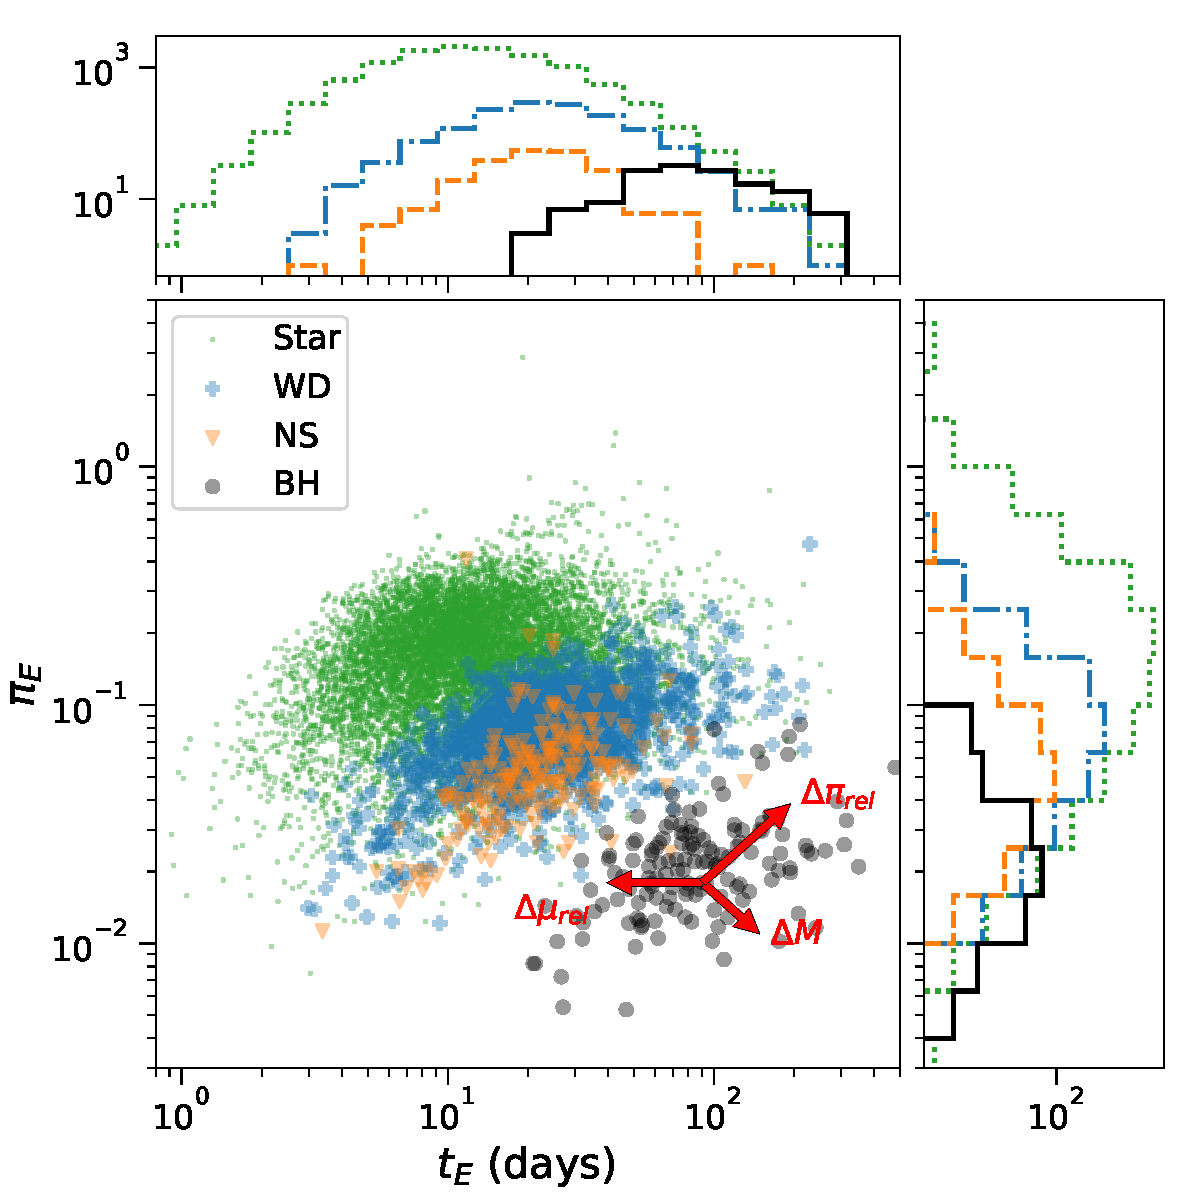
\includegraphics[width=.48\linewidth]{lam2020_tE_piE}\hspace{2mm}%
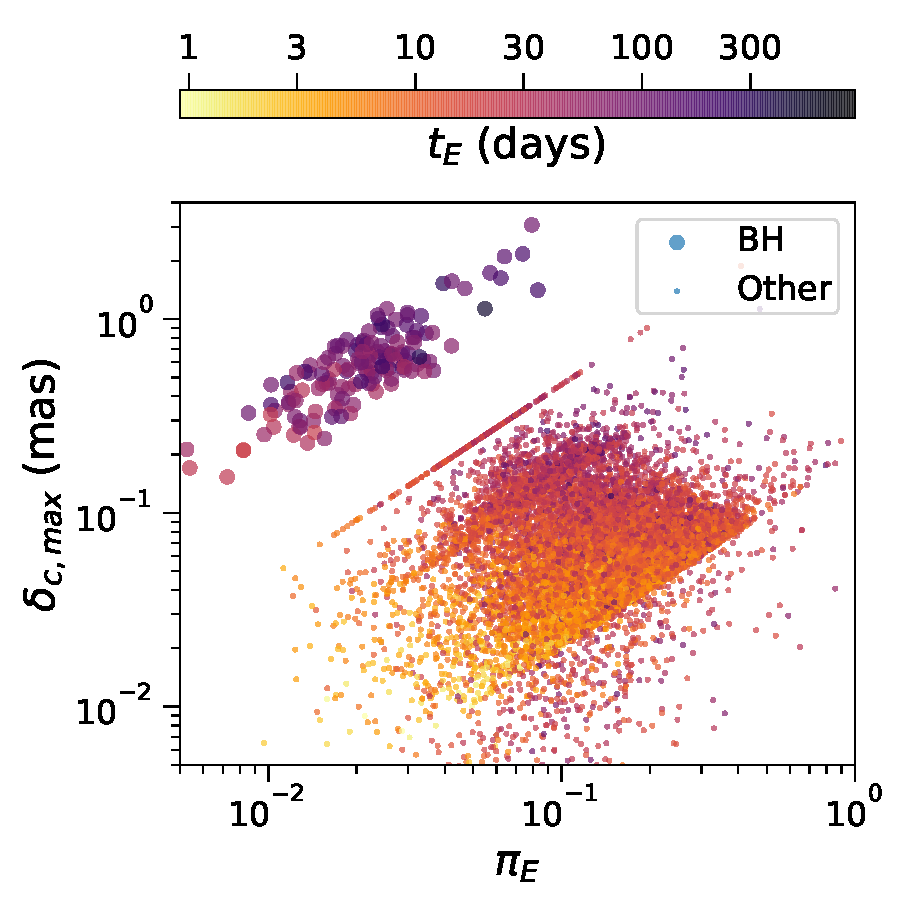
\includegraphics[width=.48\linewidth]{lam2020_deltac_piE}\\[2mm]
\credit{\ads{2020ApJ...889...31L}{Lam et al.\ 2020, ApJ 889, 31} (PopSyCLE)}
\end{column}
\begin{column}{.36\linewidth}
Black holes have
\begin{itemize}\setlength{\itemsep}{4pt}
  \item a \textbf{long} $\tE$
  \item a \textbf{small} $\piE$
  \item a \textbf{large} centroid shift
\end{itemize}
\vspace{6mm}
\uncover<2->{Long, heavy events:\\ \textbf{Roman} and \textbf{Rubin} will see them}
\end{column}
\end{columns}
\vfill
\refnote{\ads{2023ApJ...955..116L}{Lam \& Lu 2023, ApJ 955, 116}}
\note{\begin{itemize}
  \item PopSyCLE simulation of bulge events: black holes (BH) separate from stars, white dwarfs and neutron stars.
  \item Lam \& Lu 2023 predict that Roman, with HST-like astrometry over a far larger field, will measure the masses of
        hundreds of isolated black holes. Roman and Rubin have each been forecast alone; the next section shows what
        is missing: both, on the same events.
\end{itemize}}
\end{frame}

% !TeX root = ../seminar.tex
\section{Roman and Rubin}

{\setbeamercolor{background canvas}{bg=black}
\begin{frame}[plain]
\begin{tikzpicture}[remember picture, overlay]
  \node[inner sep=0] at (current page.center) {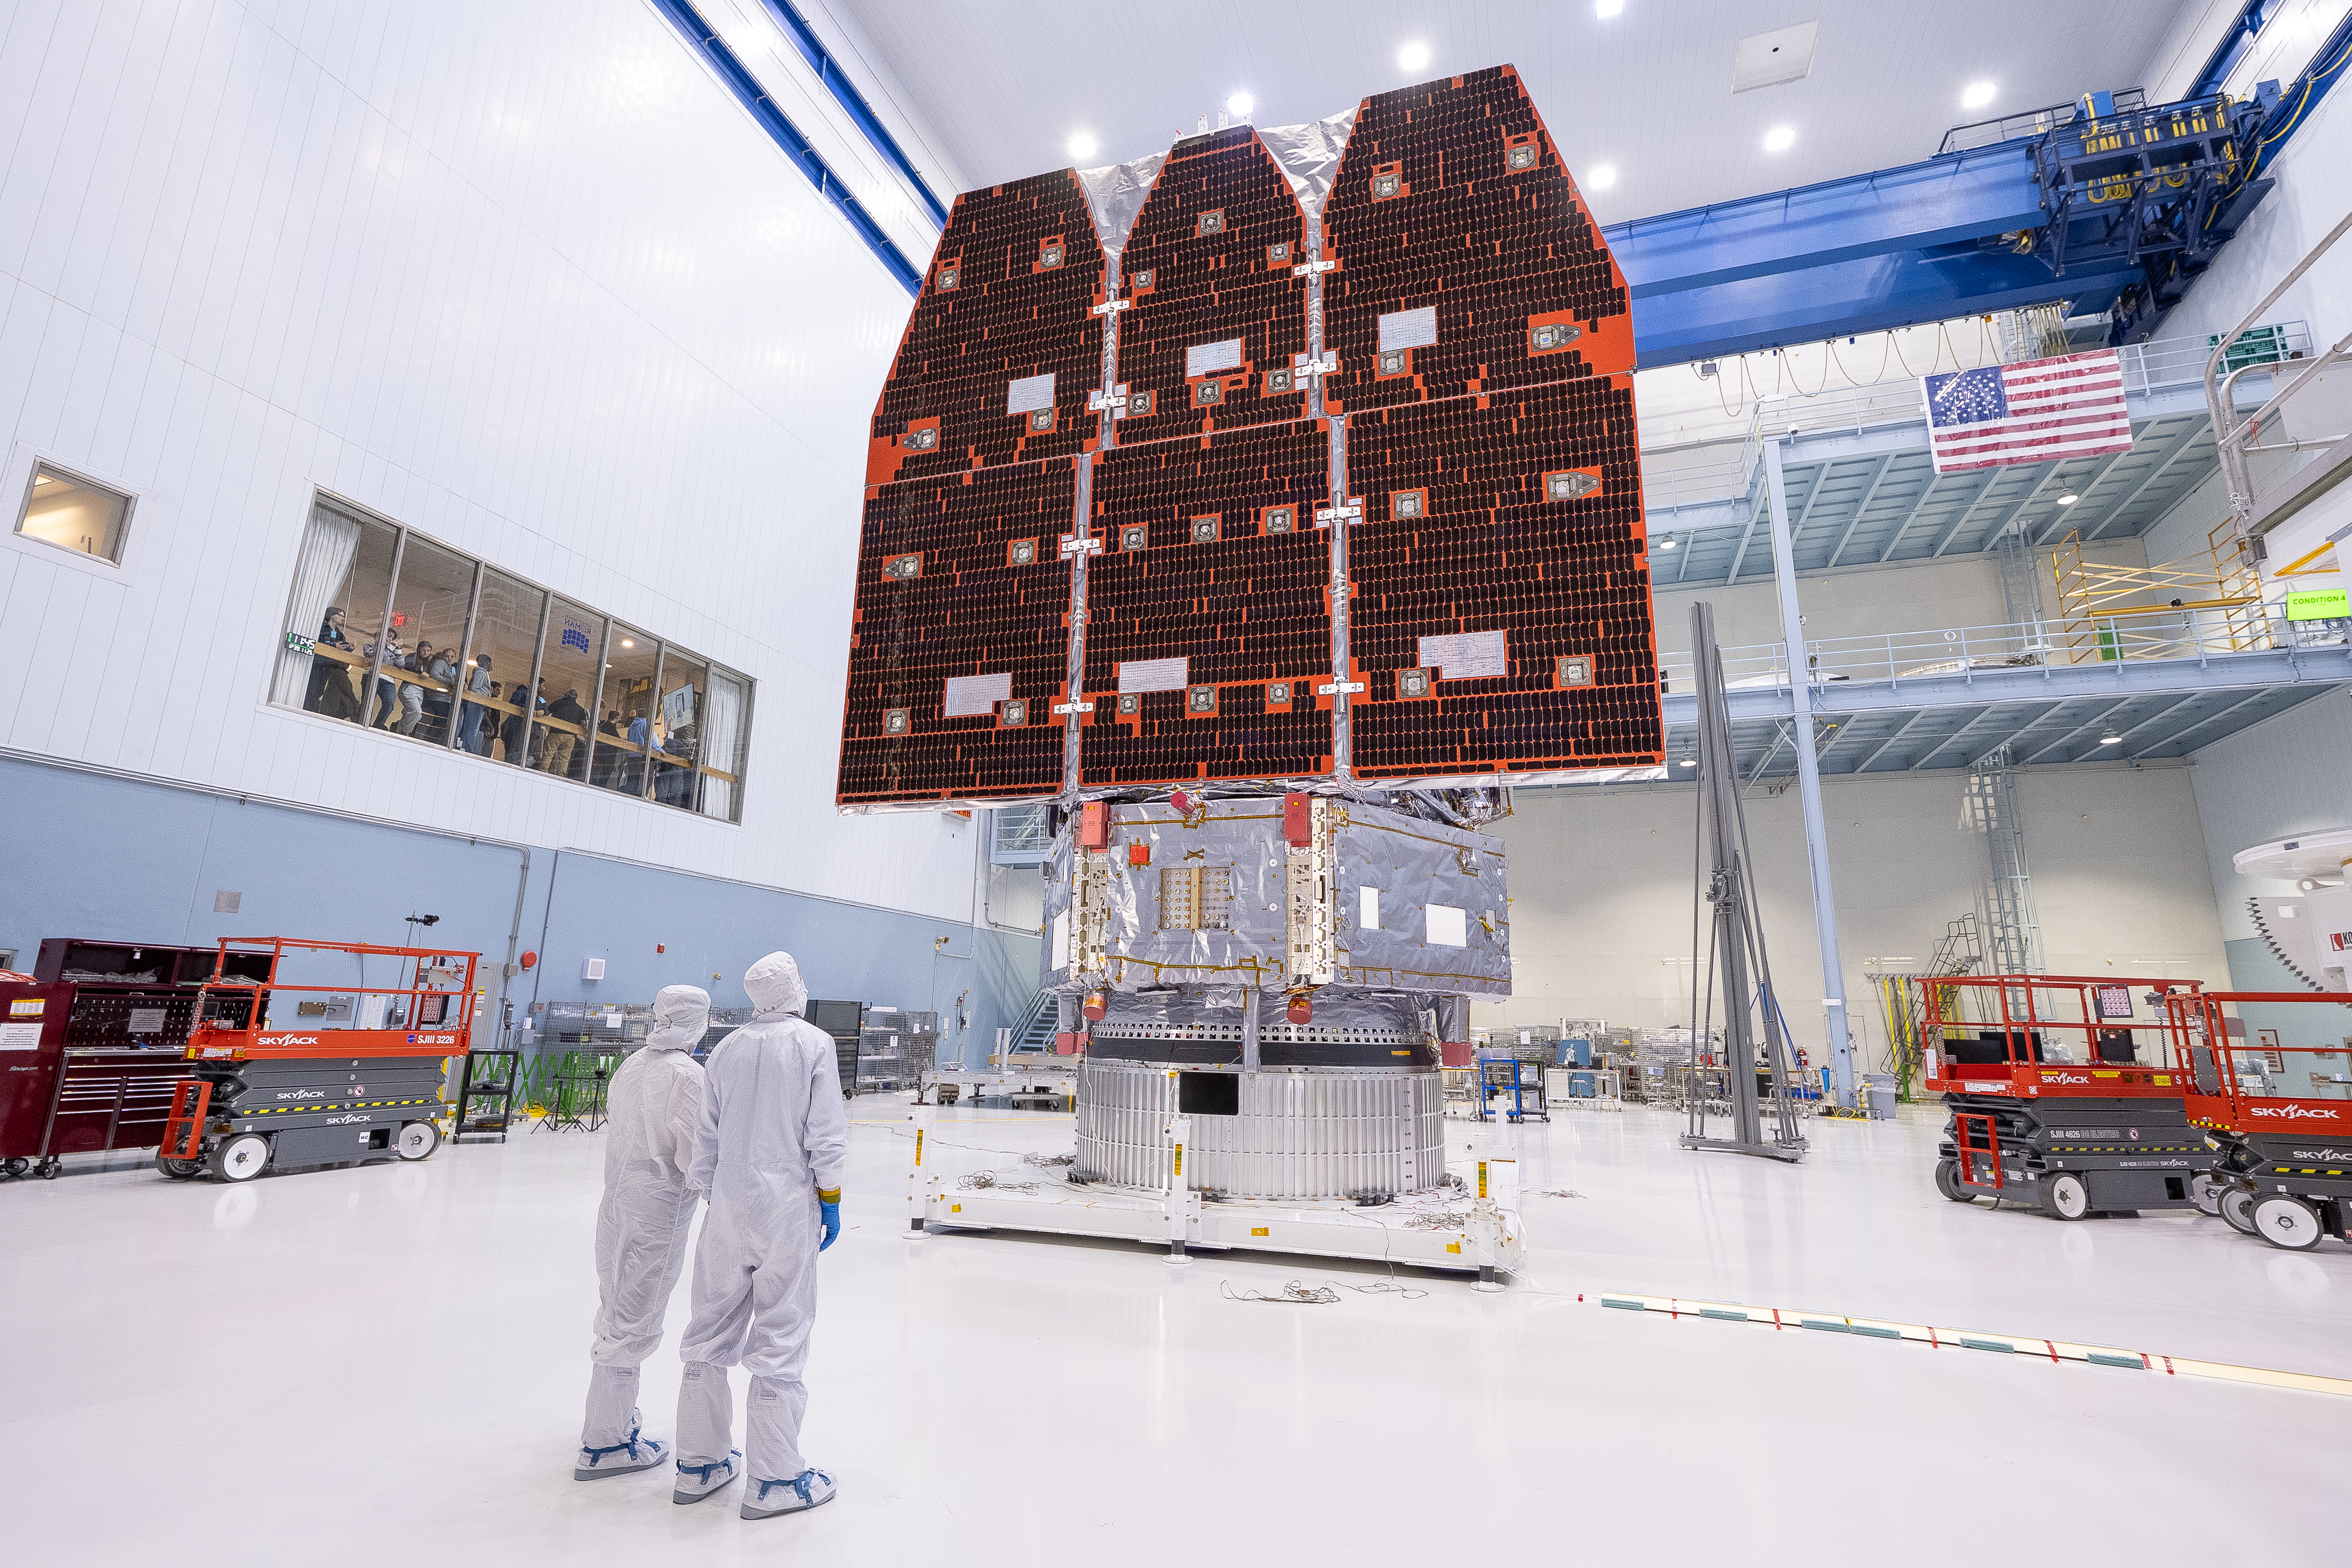
\includegraphics[width=\paperwidth]{roman_assembled}};
  \node[bleedtitle, anchor=north west] at ([xshift=5mm, yshift=-4mm]current page.north west)
       {Roman, fully assembled};
  \node[bleedtext, anchor=north west] at ([xshift=5mm, yshift=-15mm]current page.north west)
       {A $2.4$\,m mirror like \emph{Hubble}'s,\\ a field of view $\sim\!100\times$ larger};
  \bleedcredit{\href{https://www.nasa.gov/image-article/nasas-nancy-grace-roman-space-telescope-completed/}{NASA/Jolearra Tshiteya}}
  \bleedsection
\end{tikzpicture}
\note{\begin{itemize}
  \item NASA Goddard clean room, November 2025: the telescope and spacecraft joined. The technicians give the scale.
  \item Wide Field Instrument: $0.28$\,deg$^2$ per pointing, near-infrared, diffraction-limited.
\end{itemize}}
\end{frame}}


\begin{frame}{Roman's Galactic Bulge Time Domain Survey}
\vspace{2mm}
\begin{columns}[c]
\begin{column}{.56\linewidth}
\centering
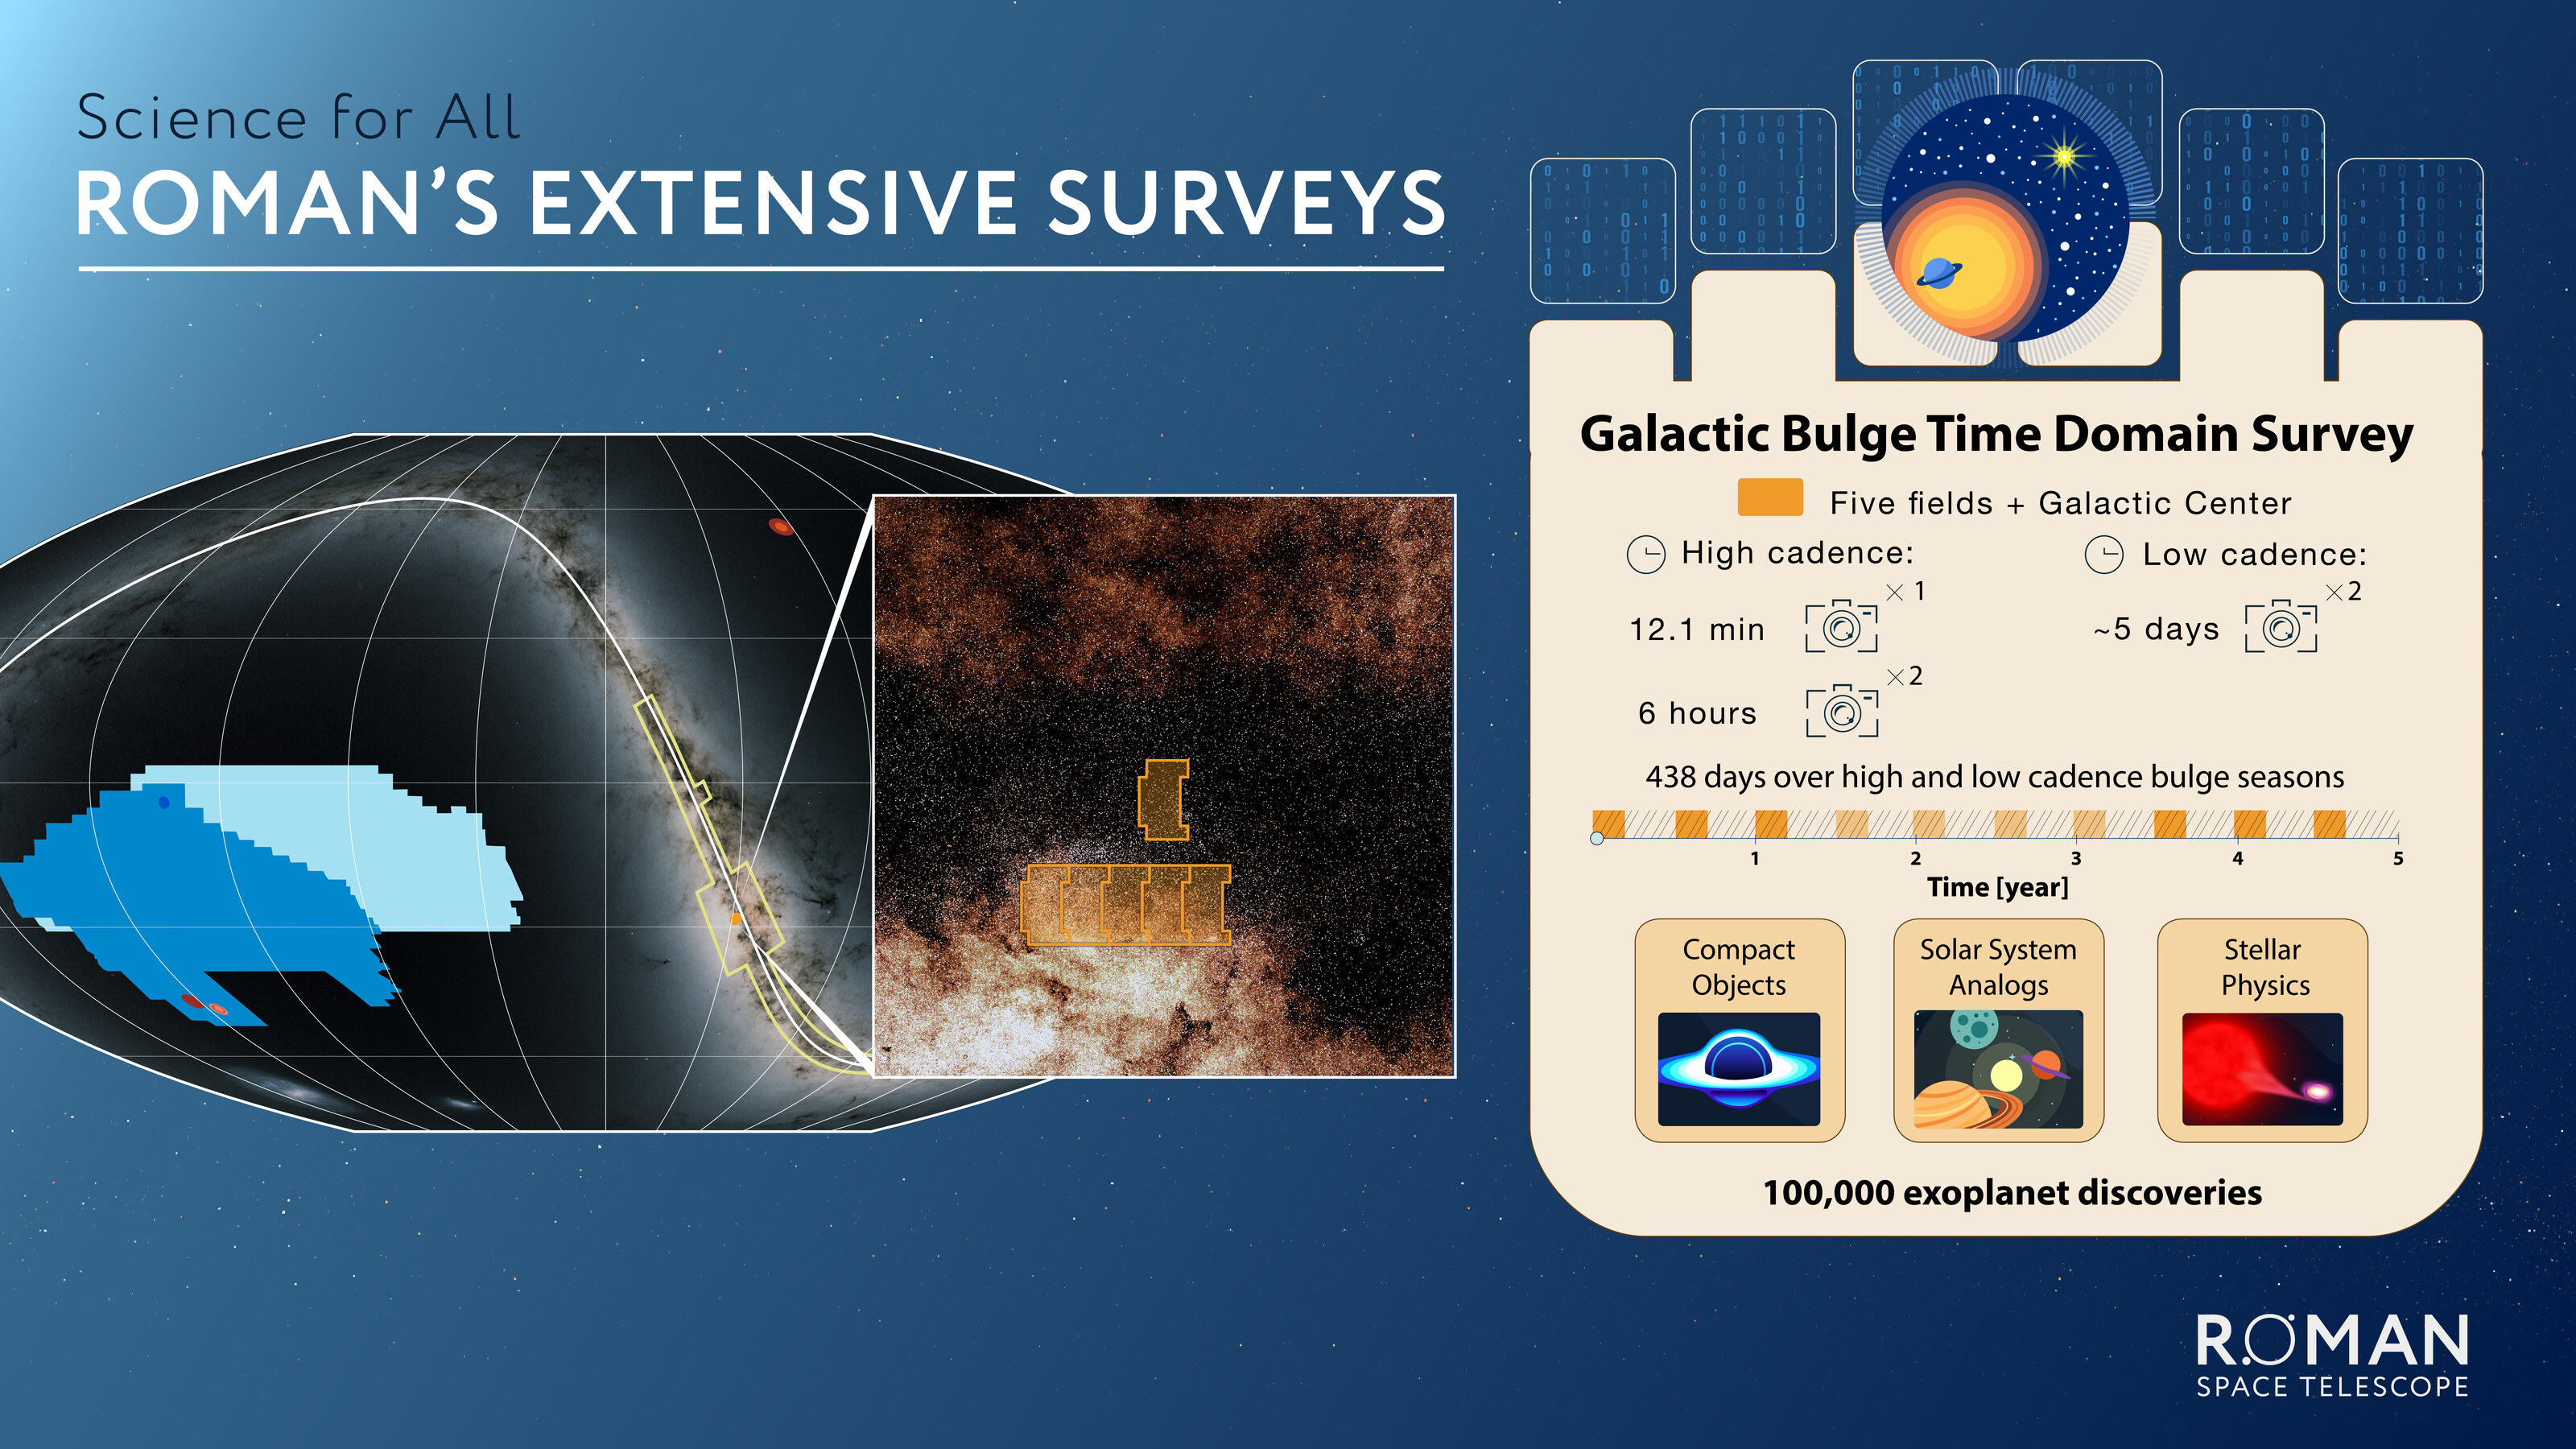
\includegraphics[width=.95\linewidth]{roman_gbtds_infographic}\\[2mm]
\credit{\href{https://roman-docs.stsci.edu/roman-community-defined-surveys/galactic-bulge-time-domain-survey}{STScI, Roman Galactic Bulge Time Domain Survey}}
\end{column}
\begin{column}{.40\linewidth}
\begin{itemize}\setlength{\itemsep}{5pt}
  \item<+-> Six fields, $1.7$\,deg$^2$
  \item<+-> Near-infrared: \textbf{little dust}
  \item<+-> An exposure every $12$\,min
  \item<+-> $\sim\!1$\,mas \textbf{astrometry}
  \item<+-> At \textbf{L2}: a second viewpoint\\ for the parallax?
\end{itemize}
\end{column}
\end{columns}
\vfill
\refnote{\ads{2019ApJS..241....3P}{Penny et al.\ 2019, ApJS 241, 3};
\ads{2019JATIS...5d4005S}{Sanderson et al.\ 2019, JATIS 5, 044005}}
\note{\begin{itemize}
  \item F146 filter: $A_{\rm F146}\approx0.20\,A_V$.
  \item Ten $\sim70$-day seasons: six at high cadence ($12.1$\,min), four at low cadence ($\sim5$\,d); gaps while the
        bulge is near the Sun. $\sim5\times10^4$ exposures per field.
  \item Diffraction-limited: $\sim1$\,mas per exposure for bright stars.
  \item L2 and Earth are $0.01$\,AU apart: a satellite parallax with Rubin was expected to help; the preliminary results test it.
\end{itemize}}
\end{frame}

{\setbeamercolor{background canvas}{bg=black}
\begin{frame}[plain]
\begin{tikzpicture}[remember picture, overlay]
  % portrait photo, full width, cropped to the band of sky and the dome (from 30% of its height down)
  \node[anchor=north, inner sep=0] at ([yshift=7.2cm]current page.north)
       {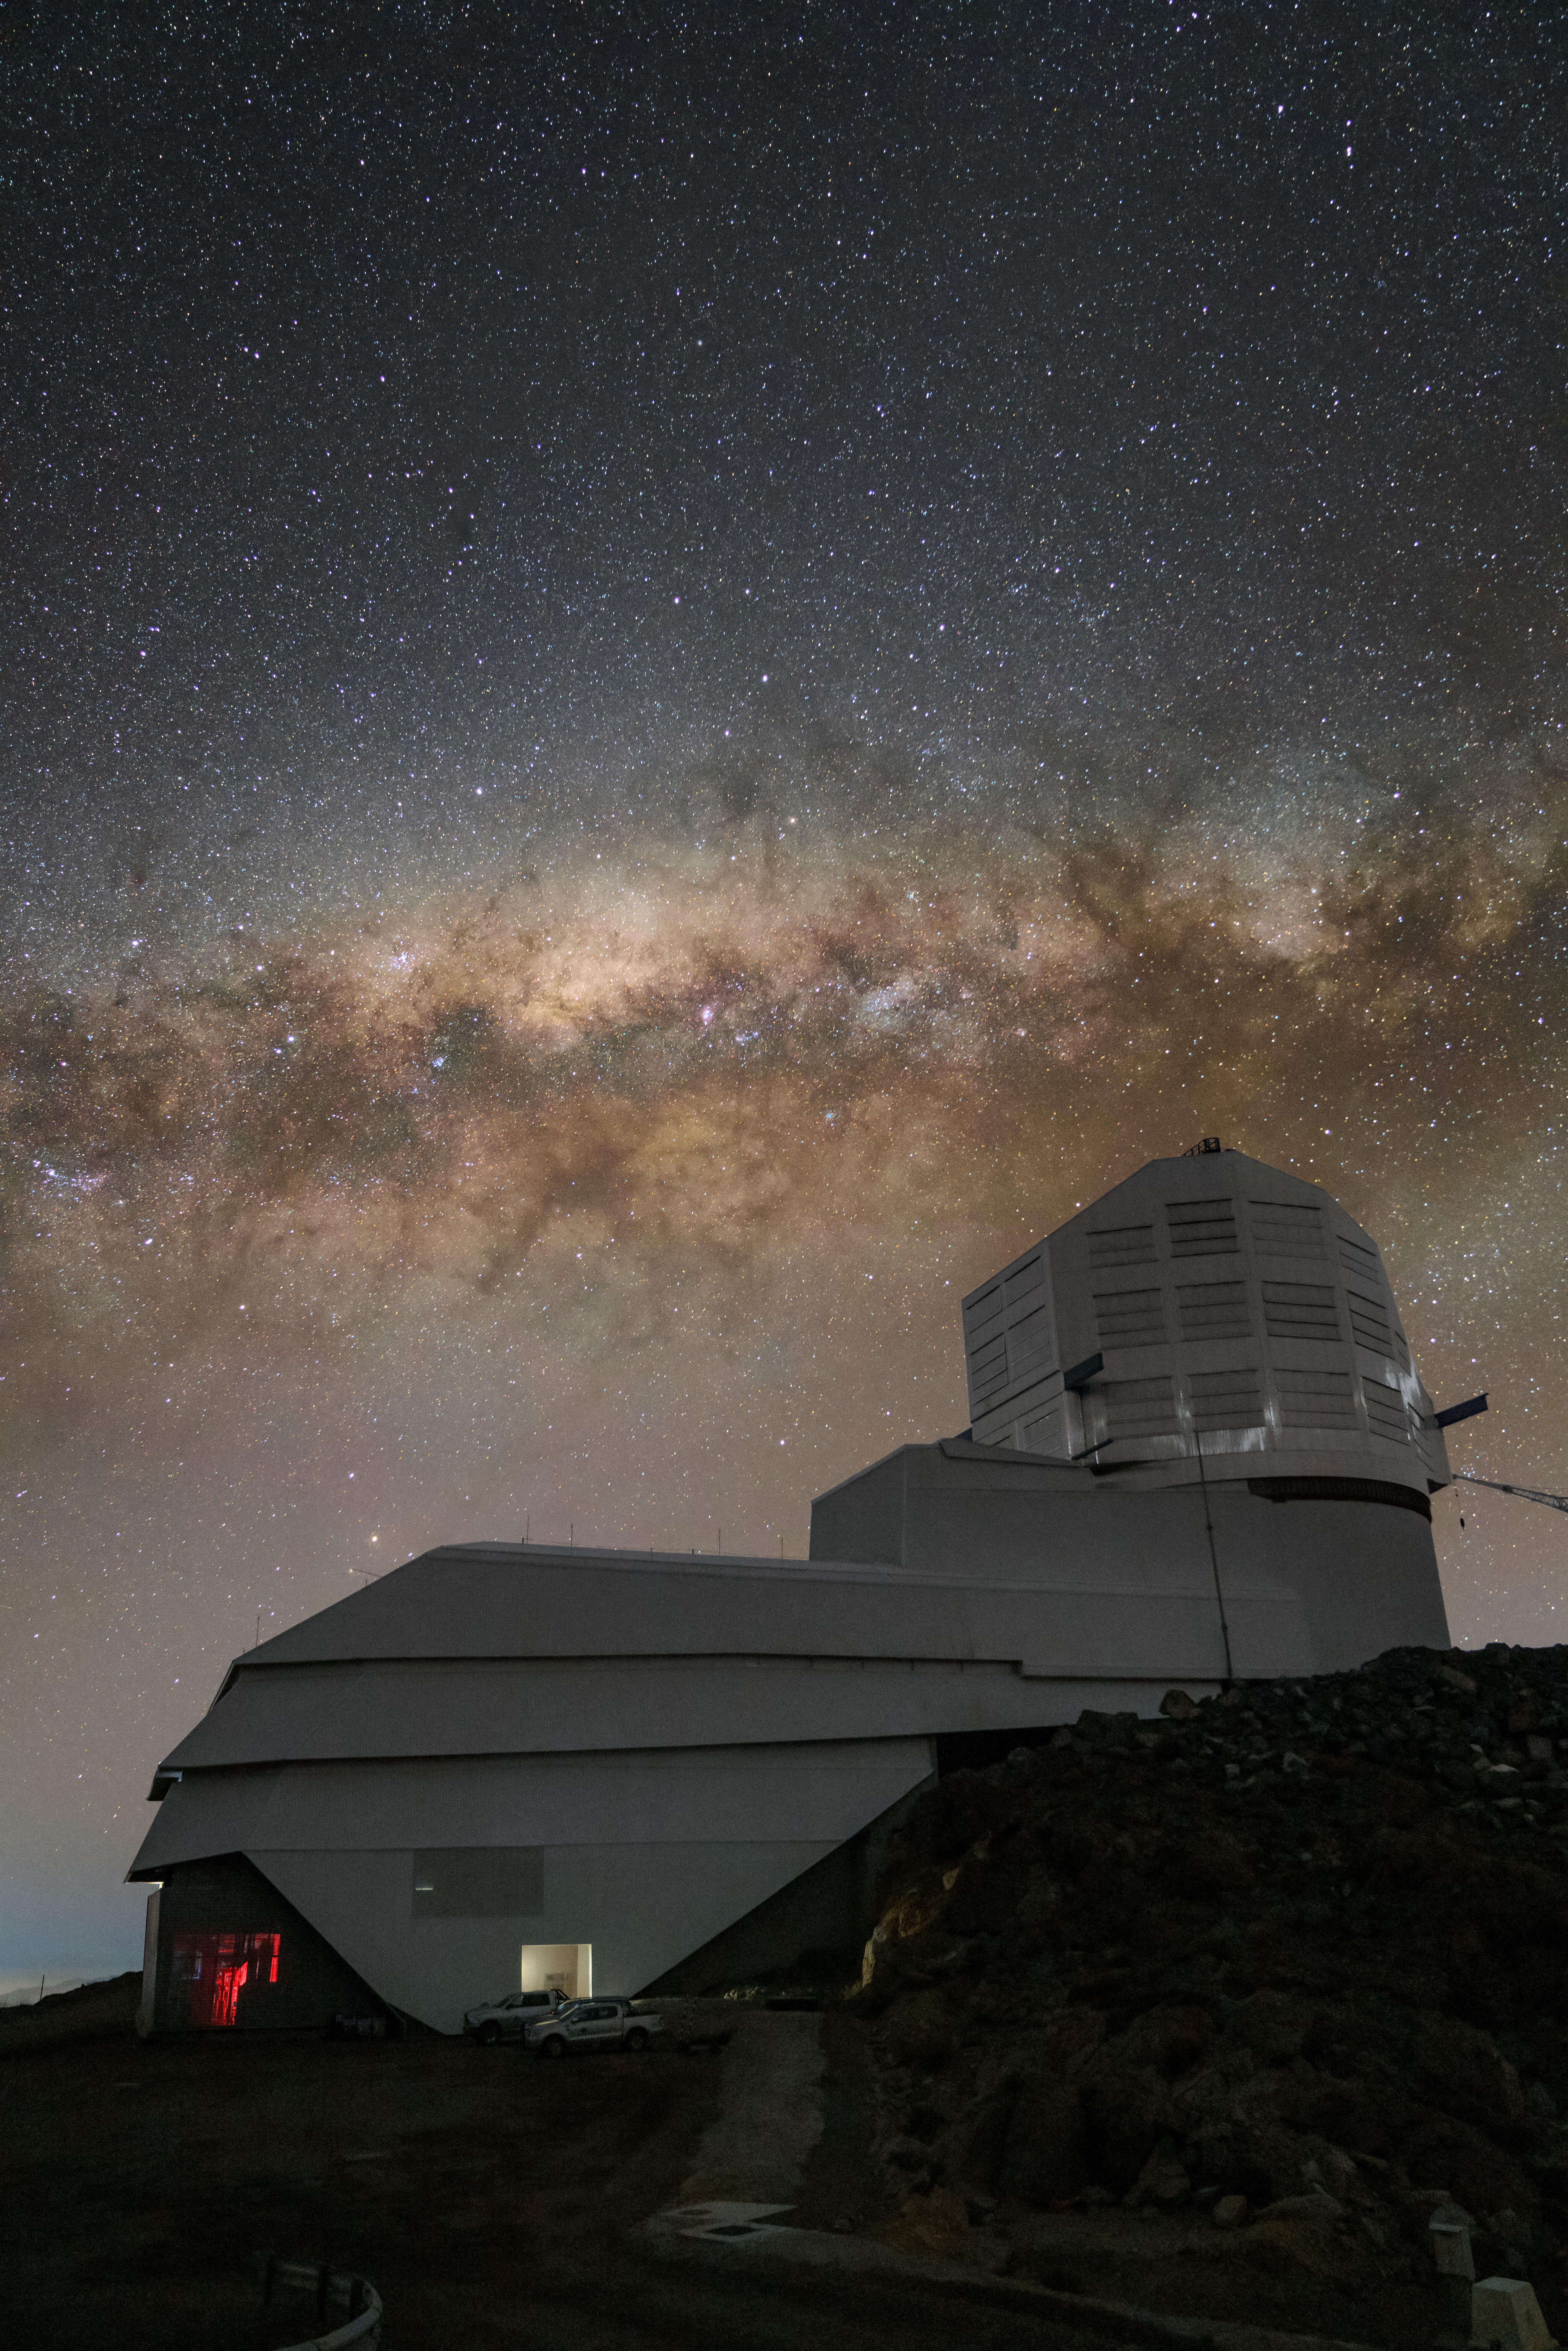
\includegraphics[width=\paperwidth]{rubin_milky_way}};
  \node[bleedtitle, anchor=north west] at ([xshift=5mm, yshift=-4mm]current page.north west)
       {Vera C.\ Rubin Observatory, Chile};
  \node[bleedtext, anchor=north west] at ([xshift=5mm, yshift=-15mm]current page.north west)
       {$8.4$\,m mirror, a $9.6$\,deg$^2$ camera:\\ the whole southern sky every few nights};
  \bleedcredit{\href{https://noirlab.edu/public/images/20220408PachonFPano35mmRubinAux_MW_EQ-001-CC-c3/}{RubinObs/NOIRLab/SLAC/NSF/DOE/AURA/P.~Hor\'alek}}
\end{tikzpicture}
\note{\begin{itemize}
  \item The Galactic bulge rising over Rubin on Cerro Pach\'on.
  \item The Legacy Survey of Space and Time: ten years, optical $ugrizy$, a 3.2-gigapixel camera.
\end{itemize}}
\end{frame}}

\begin{frame}{Rubin, and why the two complement each other}
\vspace{1mm}
\begin{columns}[c]
\begin{column}{.40\linewidth}
\centering
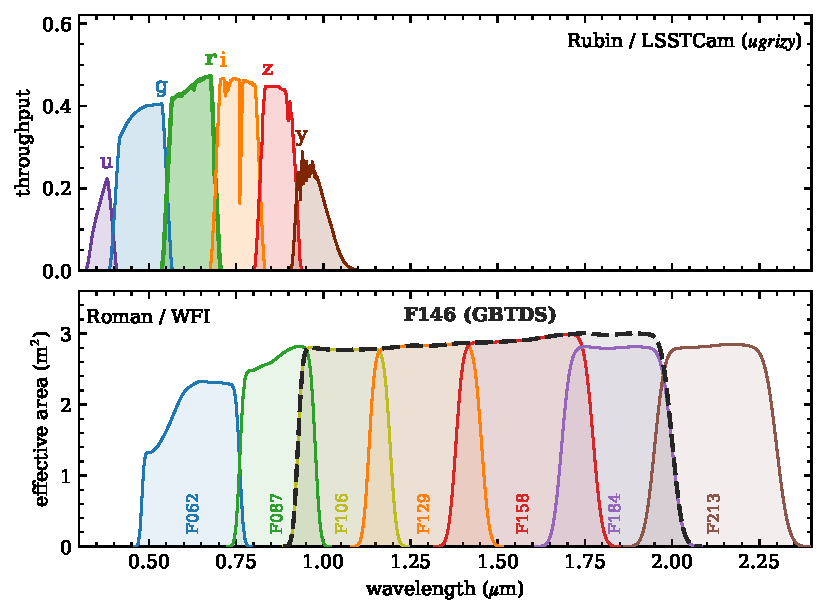
\includegraphics[width=.92\linewidth]{filters}\\[1mm]
\credit{filter curves: \href{http://svo2.cab.inta-csic.es/theory/fps/}{SVO Filter Profile Service}}
\end{column}
\begin{column}{.56\linewidth}
\centering
\textbf{Rubin LSST}: ten years, $ugrizy$, wide sky\\[3mm]
\uncover<2->{%
\renewcommand{\arraystretch}{1.15}
\begin{tabular}{@{}lcc@{}}
\toprule
 & \textbf{Roman} & \textbf{Rubin} \\
\midrule
area & small & large \\
cadence & minutes & days \\
time span & seasons & 10 years \\
dust & mild & severe \\
astrometry & $\sim$1 mas & $\gtrsim$10 mas \\
\bottomrule
\end{tabular}}
\end{column}
\end{columns}
\vspace{4mm}
\uncover<3->{%
\centering
\resizebox{.72\linewidth}{!}{% GENERATED by Report/overview/make_timeline.py -- do not edit.
% sightline (l,b) = (0.40, -1.45); Rubin 2387 epochs, Roman 50401 epochs.
\def\tlL{0.4}\def\tlB{-1.4}\def\tlNrub{2{,}387}\def\tlNrom{50{,}401}
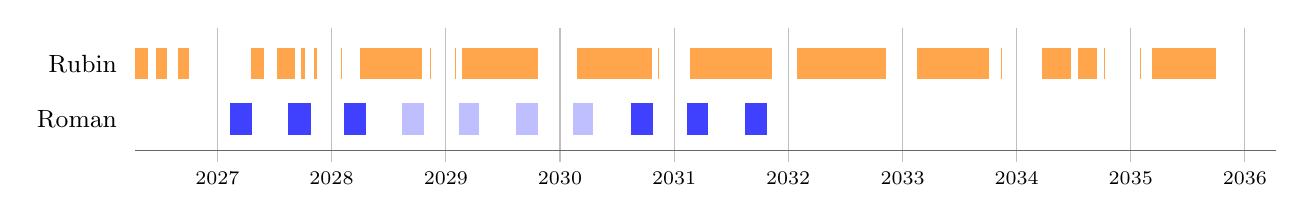
\begin{tikzpicture}[x=1cm,y=1cm]
\draw[black!25] (1.052,-0.15) -- (1.052,1.55);\node[font=\scriptsize,anchor=north] at (1.052,-0.15) {2027};
\draw[black!25] (2.501,-0.15) -- (2.501,1.55);\node[font=\scriptsize,anchor=north] at (2.501,-0.15) {2028};
\draw[black!25] (3.954,-0.15) -- (3.954,1.55);\node[font=\scriptsize,anchor=north] at (3.954,-0.15) {2029};
\draw[black!25] (5.403,-0.15) -- (5.403,1.55);\node[font=\scriptsize,anchor=north] at (5.403,-0.15) {2030};
\draw[black!25] (6.852,-0.15) -- (6.852,1.55);\node[font=\scriptsize,anchor=north] at (6.852,-0.15) {2031};
\draw[black!25] (8.301,-0.15) -- (8.301,1.55);\node[font=\scriptsize,anchor=north] at (8.301,-0.15) {2032};
\draw[black!25] (9.754,-0.15) -- (9.754,1.55);\node[font=\scriptsize,anchor=north] at (9.754,-0.15) {2033};
\draw[black!25] (11.203,-0.15) -- (11.203,1.55);\node[font=\scriptsize,anchor=north] at (11.203,-0.15) {2034};
\draw[black!25] (12.652,-0.15) -- (12.652,1.55);\node[font=\scriptsize,anchor=north] at (12.652,-0.15) {2035};
\draw[black!25] (14.101,-0.15) -- (14.101,1.55);\node[font=\scriptsize,anchor=north] at (14.101,-0.15) {2036};
\draw[black!60] (0,0) -- (14.5,0);
\node[font=\small,anchor=east] at (-0.1,1.1) {Rubin};
\node[font=\small,anchor=east] at (-0.1,0.4) {Roman};
\fill[orange!70] (0.000,0.9) rectangle (0.167,1.3);
\fill[orange!70] (0.270,0.9) rectangle (0.408,1.3);
\fill[orange!70] (0.555,0.9) rectangle (0.686,1.3);
\fill[orange!70] (1.481,0.9) rectangle (1.644,1.3);
\fill[orange!70] (1.809,0.9) rectangle (2.036,1.3);
\fill[orange!70] (2.119,0.9) rectangle (2.170,1.3);
\fill[orange!70] (2.285,0.9) rectangle (2.317,1.3);
\fill[orange!70] (2.620,0.9) rectangle (2.628,1.3);
\fill[orange!70] (2.858,0.9) rectangle (3.647,1.3);
\fill[orange!70] (3.746,0.9) rectangle (3.754,1.3);
\fill[orange!70] (4.065,0.9) rectangle (4.073,1.3);
\fill[orange!70] (4.153,0.9) rectangle (5.128,1.3);
\fill[orange!70] (5.614,0.9) rectangle (6.569,1.3);
\fill[orange!70] (6.652,0.9) rectangle (6.660,1.3);
\fill[orange!70] (7.051,0.9) rectangle (8.098,1.3);
\fill[orange!70] (8.417,0.9) rectangle (9.543,1.3);
\fill[orange!70] (9.941,0.9) rectangle (10.849,1.3);
\fill[orange!70] (11.004,0.9) rectangle (11.011,1.3);
\fill[orange!70] (11.529,0.9) rectangle (11.897,1.3);
\fill[orange!70] (11.981,0.9) rectangle (12.219,1.3);
\fill[orange!70] (12.314,0.9) rectangle (12.322,1.3);
\fill[orange!70] (12.768,0.9) rectangle (12.776,1.3);
\fill[orange!70] (12.926,0.9) rectangle (13.731,1.3);
\fill[blue!75] (1.215,0.2) rectangle (1.489,0.6);
\fill[blue!75] (1.949,0.2) rectangle (2.235,0.6);
\fill[blue!75] (2.665,0.2) rectangle (2.939,0.6);
\fill[blue!25] (3.399,0.2) rectangle (3.677,0.6);
\fill[blue!25] (4.115,0.2) rectangle (4.373,0.6);
\fill[blue!25] (4.849,0.2) rectangle (5.127,0.6);
\fill[blue!25] (5.565,0.2) rectangle (5.823,0.6);
\fill[blue!75] (6.299,0.2) rectangle (6.585,0.6);
\fill[blue!75] (7.015,0.2) rectangle (7.289,0.6);
\fill[blue!75] (7.749,0.2) rectangle (8.035,0.6);
\end{tikzpicture}
}\\[1mm]
\refnote{One sightline in Roman's fields: Rubin's visits (orange), Roman's seasons (blue; dark = high cadence).
\quad Rubin: \ads{2019ApJ...873..111I}{Ivezi\'c et al.\ 2019, ApJ 873, 111}}}
\note{\begin{itemize}
  \item Rubin: $9.6$\,deg$^2$ field of view, from the ground; $\sim2{,}400$ visits per bulge sightline, every few days
        while the bulge is up.
  \item Seeing-limited: $\gtrsim10$\,mas astrometry per visit.
  \item Optical bands are heavily extincted toward the bulge: $A_r\approx0.85\,A_V$ against $0.20\,A_V$ for F146.
\end{itemize}}
\end{frame}

\begin{frame}{What has been forecast so far}
\vspace{2mm}
\begin{columns}[T]
\begin{column}{.32\linewidth}
\centering
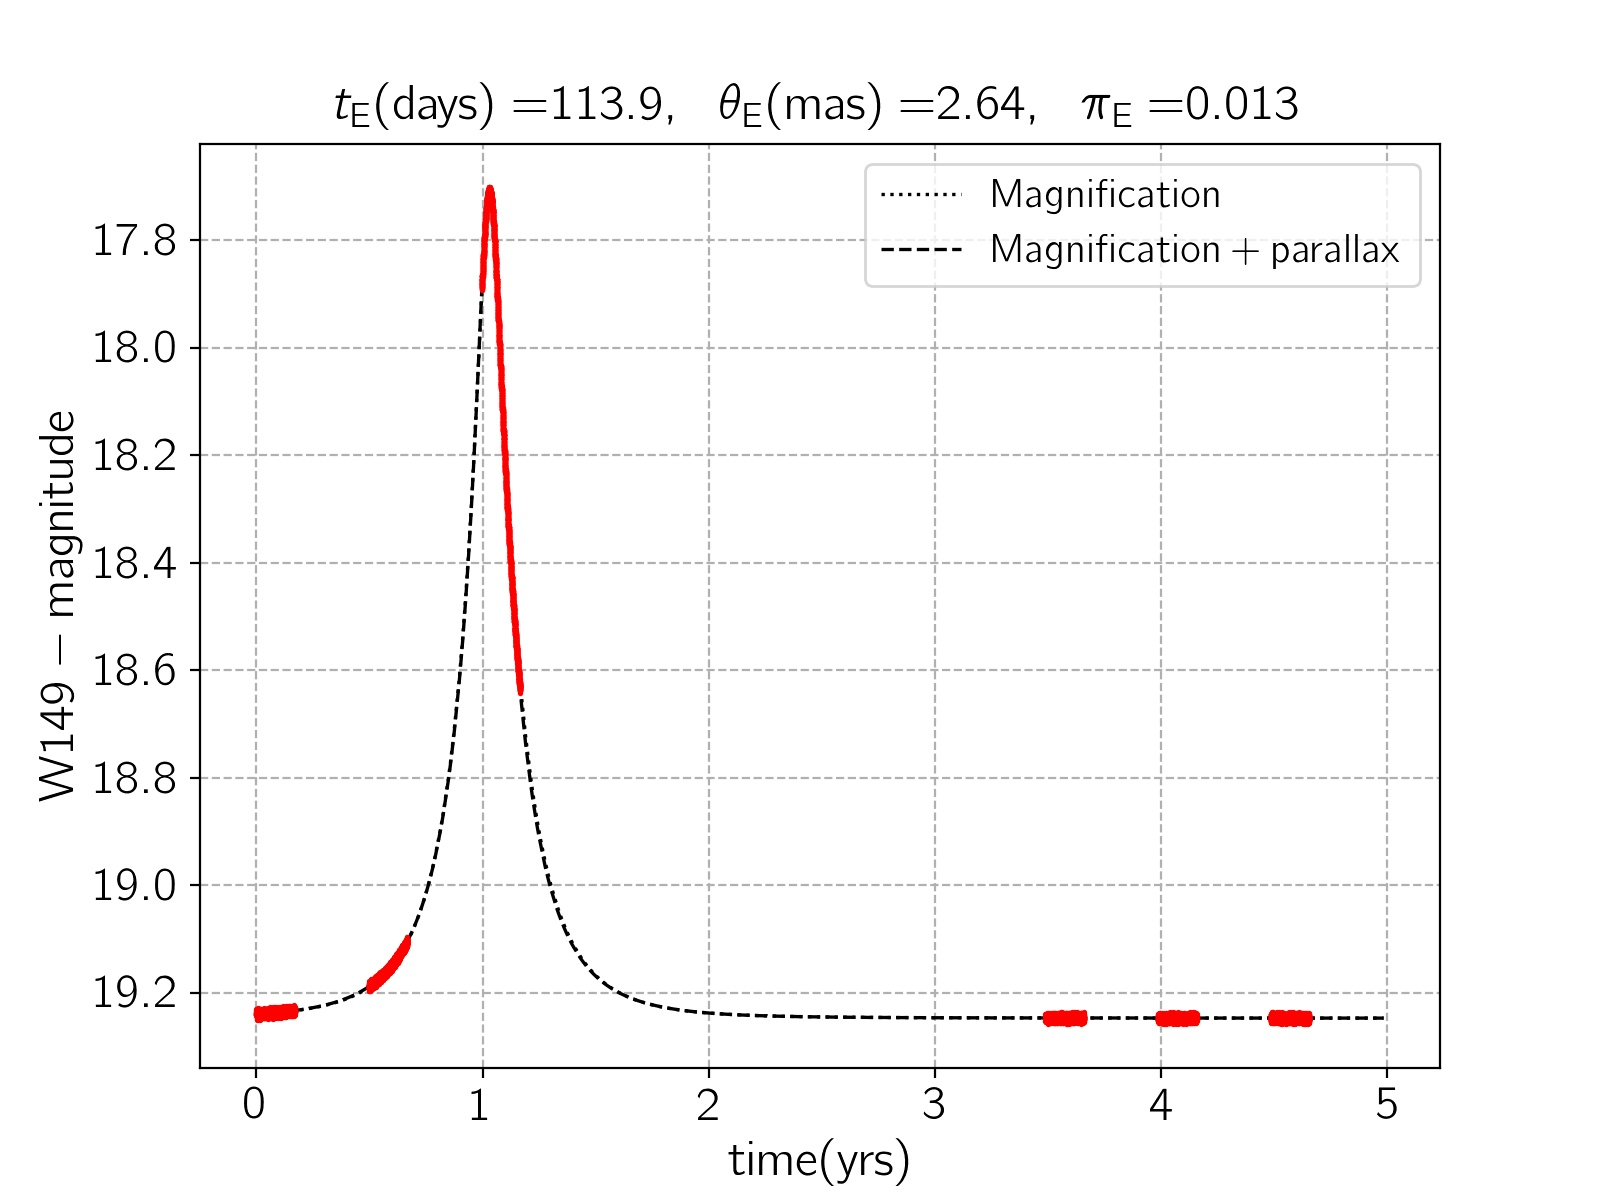
\includegraphics[height=3.2cm]{ss23_lightcurve}\\[1mm]
\credit{\ads{2023AJ....165...96S}{Sajadian \& Sahu 2023}}\\[3mm]
\textbf{Roman}: black-hole masses
\end{column}
\begin{column}{.32\linewidth}
\centering
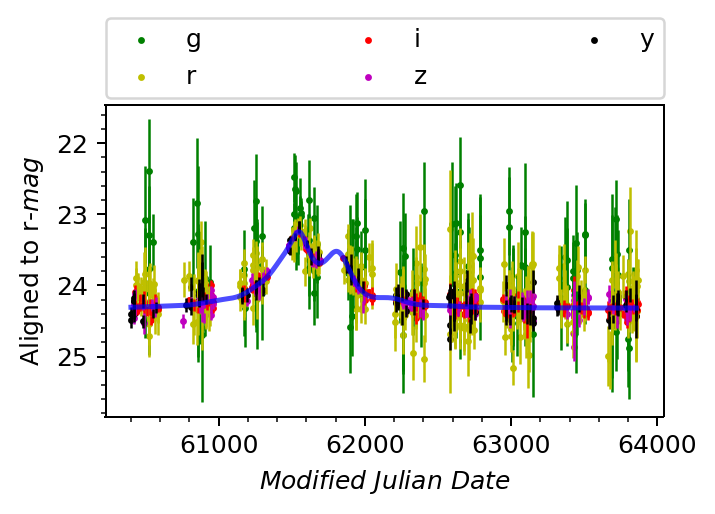
\includegraphics[height=3.2cm]{abrams2025_example}\\[1mm]
\credit{\ads{2025ApJS..276...10A}{Abrams et al.\ 2025}}\\[3mm]
\textbf{Rubin}: characterising events
\end{column}
\begin{column}{.32\linewidth}
\centering
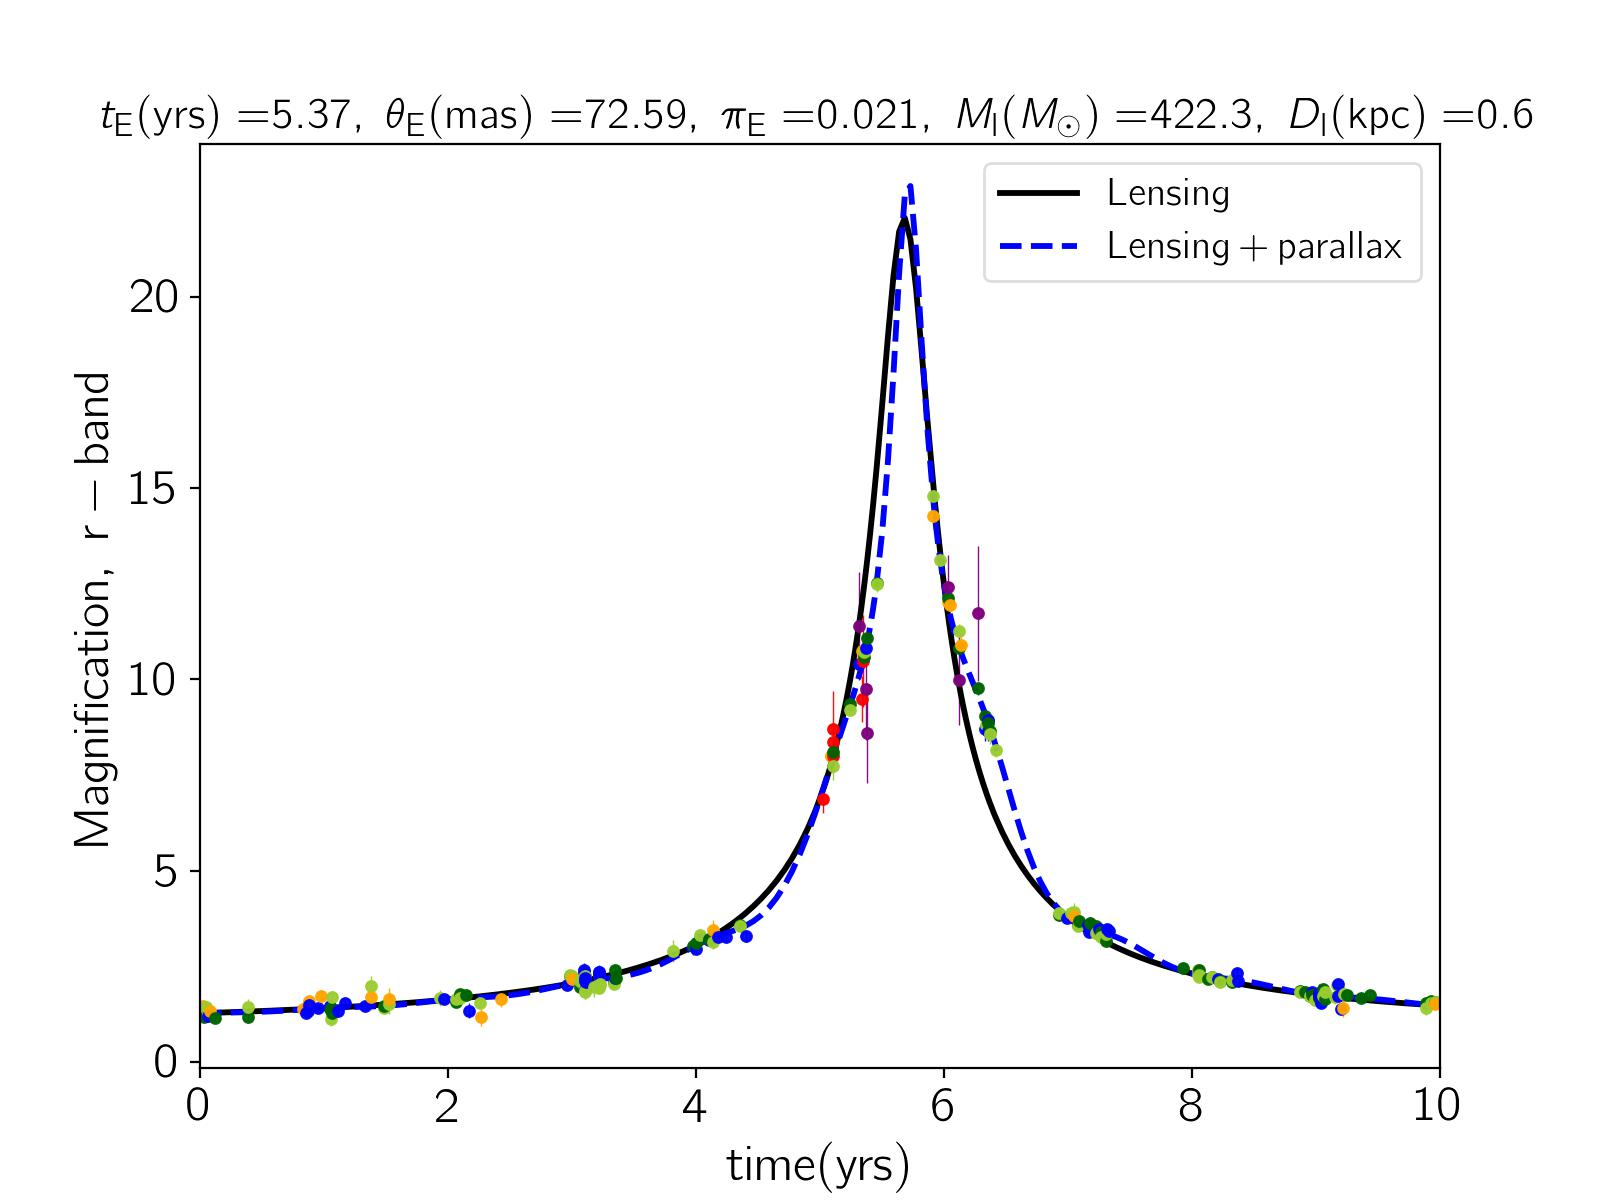
\includegraphics[height=3.2cm]{sm26_lightcurve}\\[1mm]
\credit{\ads{2026ApJ..1009..116S}{Sajadian \& Makler 2026}}\\[3mm]
\textbf{Rubin}: black holes, two images
\end{column}
\end{columns}
\vspace{6mm}
\uncover<2->{%
\begin{beamercolorbox}[rounded=true,sep=6pt,wd=\linewidth]{block body alerted}
\centering
Each telescope alone. \textbf{This thesis: both, on the same events.}
\end{beamercolorbox}}
\note{\begin{itemize}
  \item Sajadian \& Sahu 2023 (AJ 165, 96): Roman alone, isolated black holes; photometric + astrometric Fisher
        forecasts. For $dN/dM\propto M^{-1}$: $\tetE$ to 10\% for $\sim99\%$, the mass for $\sim30\%$ of detections.
  \item Abrams et al.\ 2025 (ApJS 276, 10): which LSST strategies characterise events ($\tE$ and $\piE$) across the
        Galactic plane.
  \item Sajadian \& Makler 2026 (ApJ 1009, 116): Rubin, black holes toward the Magellanic Clouds; images resolvable for
        1.4\% (LMC) and 16.3\% (SMC) of black-hole events.
  \item The thesis: who detects what, what each adds to the other, how many black-hole masses the combination gives.
\end{itemize}}
\end{frame}

% !TeX root = ../seminar.tex
\section{The Simulation}
\frame{\sectionpage}

\begin{frame}{A Monte Carlo of the bulge sky}
\centering
\vspace{1mm}
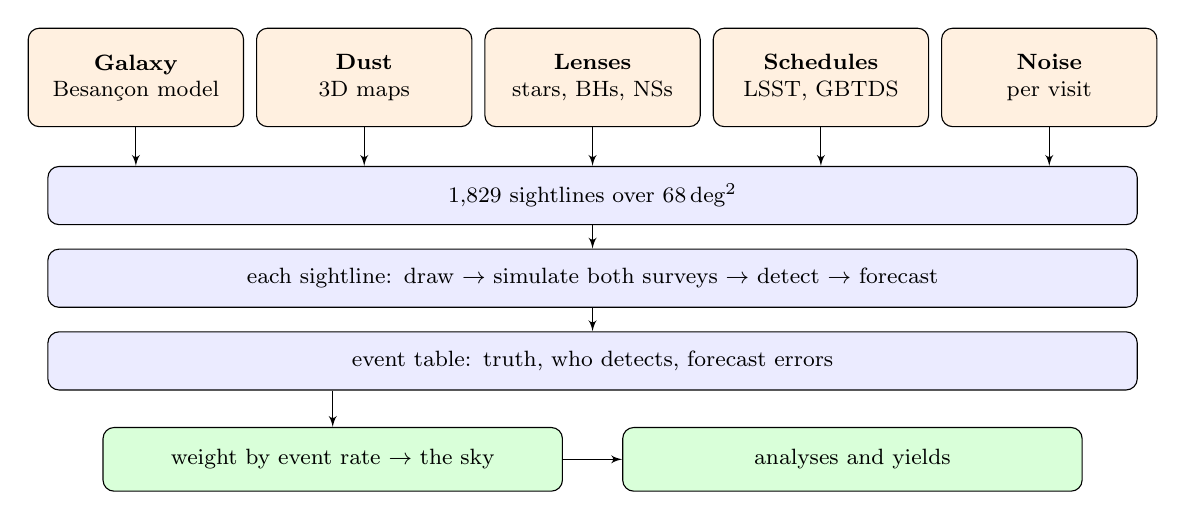
\begin{tikzpicture}[font=\footnotesize, execute at begin node={\hyphenpenalty=10000},
    inb/.style={terminator, fill=orange!12, text width=2.5cm, align=center, minimum height=1.25cm},
    row/.style={terminator, fill=blue!8, text width=13.6cm, align=center, minimum height=2.1em},
    resb/.style={terminator, fill=green!15, align=center, minimum height=2.3em}]
  \node[inb] (g) at (0,0)     {\textbf{Galaxy}\\ Besan\c{c}on model};
  \node[inb] (d) at (2.9,0)   {\textbf{Dust}\\ 3D maps};
  \node[inb] (p) at (5.8,0)   {\textbf{Lenses}\\ stars, BHs, NSs};
  \node[inb] (s) at (8.7,0)   {\textbf{Schedules}\\ LSST, GBTDS};
  \node[inb] (e) at (11.6,0)  {\textbf{Noise}\\ per visit};
  \uncover<2->{
  \node[row] (sky) at (5.8,-1.5) {$1{,}829$ sightlines over $68$\,deg$^2$};
  \foreach \n in {g,d,p,s,e} \path[connector] (\n.south) -- (\n.south |- sky.north);}
  \uncover<3->{
  \node[row] (mc) at (5.8,-2.55) {each sightline: draw $\to$ simulate both surveys $\to$ detect $\to$ forecast};
  \path[connector] (sky) -- (mc);}
  \uncover<4->{
  \node[row] (tab) at (5.8,-3.6) {event table: truth, who detects, forecast errors};
  \path[connector] (mc) -- (tab);}
  \uncover<5->{
  \node[resb, text width=5.6cm] (w) at (2.5,-4.85) {weight by event rate $\to$ the sky};
  \node[resb, text width=5.6cm] (an) at (9.1,-4.85) {analyses and yields};
  \path[connector] (tab.south -| w.north) -- (w.north);
  \path[connector] (w) -- (an);}
\end{tikzpicture}
\vfill
\refnote{Built on Dr.\ Sajadian's microlensing simulation (Magellanic Clouds), extended to two observatories.
\ads{2003A\%26A...409..523R}{Robin et al.\ 2003};
\ads{2019ApJ...887...93G}{Green et al.\ 2019};
\ads{2025ApJ...992...39Z}{Zucker et al.\ 2025};
\ads{1989ApJ...345..245C}{Cardelli et al.\ 1989}}
\note{\begin{itemize}
  \item Galaxy: Besan\c{c}on densities and a synthetic colour--magnitude diagram; magnitudes in $ugrizy$ and F146.
  \item Dust: $A_V(D)$ from Bayestar and DECaPS, converted with the CCM89 law.
  \item Lenses: ordinary stars and remnants, black holes, or neutron stars (one population per run).
  \item Schedules: Rubin's simulated LSST visit list; Roman's GBTDS seasons, fields and cadence.
  \item Sky: $0.1^\circ$ grid inside Roman's fields, $0.2^\circ$ outside; each sightline carries its area.
  \item The Monte Carlo does not draw events in proportion to the rate, so every event is weighted by its event rate.
\end{itemize}}
\end{frame}

\begin{frame}{Simulating one event}
\centering
\vspace{2mm}
\begin{tikzpicture}[font=\footnotesize, execute at begin node={\hyphenpenalty=10000},
    st/.style={terminator, fill=blue!8, text width=2.7cm, align=center, minimum height=3.2em},
    q/.style={terminator, fill=yellow!25, text width=2.7cm, align=center, minimum height=3.2em},
    nb/.style={draw=none, font=\scriptsize\itshape, text=jdgrey}]
  \node[st] (src) at (0,0)     {\textbf{Source}\\ star, distance, dust};
  \node[st] (len) at (3.75,0)  {\textbf{Lens}\\ mass, distance, velocity};
  \node[q]  (vis) at (7.5,0)   {\textbf{Visible?}};
  \node[st] (dat) at (11.25,0) {\textbf{Data}\\ at every real visit};
  \node[q]  (det) at (11.25,-2.2) {\textbf{Detected?}\\ $\Delta\chi^2\ge500$};
  \node[st] (fis) at (7.5,-2.2)   {\textbf{Fisher forecast}\\ three times};
  \node[st] (row) at (3.75,-2.2)  {\textbf{Event table}};
  \node[q]  (done) at (0,-2.2)    {\textbf{Enough events?}};
  \path[connector] (src) -- (len);
  \path[connector] (len) -- (vis);
  \path[connector] (vis) -- node[nb, above] {yes} (dat);
  \path[connector] (dat) -- (det);
  \path[connector] (det) -- node[nb, above] {yes} (fis);
  \path[connector] (fis) -- (row);
  \path[connector] (row) -- (done);
  \path[connector] (done) -- node[nb, left] {no} (src);
\end{tikzpicture}

\vspace{8mm}
\uncover<2->{Rubin from \textbf{Earth}, Roman from \textbf{L2}: two slightly different light curves}
\vfill
\refnote{Detection criterion as in \ads{2019ApJS..241....3P}{Penny et al.\ 2019, ApJS 241, 3}}
\note{\begin{itemize}
  \item Lens distance drawn in proportion to the event rate; $u_0\le3$; $t_0$ anywhere in the ten years.
  \item Visible: bright enough at the peak and not saturated, in two Rubin bands or in Roman's F146.
  \item Data: magnification and centroid shift with parallax at every real visit; each instrument's noise added.
  \item Detected: $\Delta\chi^2\ge500$ against a constant star and three consecutive points above $3\sigma$; tested on
        Rubin's data, Roman's and both. Every draw is kept, detected or not, for efficiencies.
  \item Labels: detected by Rubin only, Roman only, both, or only jointly.
\end{itemize}}
\end{frame}

\begin{frame}{Forecasting the measurement: three Fisher matrices}
\vspace{2mm}
\begin{columns}[c]
\begin{column}{.42\linewidth}
\centering
Curvature of $\chi^2$ at the truth:
\[
  F_{jk} = \sum_i \frac{1}{\sigma_i^2}\,\frac{\partial m_i}{\partial\theta_j}\,\frac{\partial m_i}{\partial\theta_k}
\]
\[
  C = F^{-1}
\]
\vspace{2mm}
\uncover<2->{\textbf{characterised:}\\ $\tE>2\sigma_{\tE}$ and $\piE>2\sigma_{\piE}$}
\end{column}
\begin{column}{.54\linewidth}
\centering
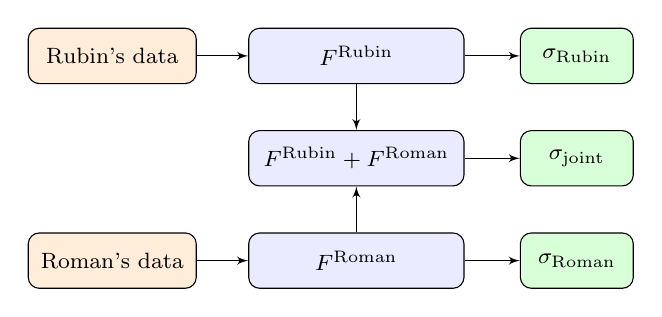
\begin{tikzpicture}[font=\footnotesize,
    d/.style={terminator, fill=orange!15, text width=1.9cm, align=center},
    f/.style={terminator, fill=blue!8, text width=2.5cm, align=center},
    s/.style={terminator, fill=green!15, text width=1.2cm, align=center}]
  \node[d] (rd) at (0,1.3)  {Rubin's data};
  \node[d] (od) at (0,-1.3) {Roman's data};
  \node[f] (fr) at (3.1,1.3)  {$F^{\rm Rubin}$};
  \node[f] (fo) at (3.1,-1.3) {$F^{\rm Roman}$};
  \node[f] (fj) at (3.1,0)    {$F^{\rm Rubin}+F^{\rm Roman}$};
  \node[s] (sr) at (5.9,1.3)  {$\sigma_{\rm Rubin}$};
  \node[s] (sj) at (5.9,0)    {$\sigma_{\rm joint}$};
  \node[s] (so) at (5.9,-1.3) {$\sigma_{\rm Roman}$};
  \path[connector] (rd) -- (fr); \path[connector] (od) -- (fo);
  \path[connector] (fr) -- (fj); \path[connector] (fo) -- (fj);
  \path[connector] (fr) -- (sr); \path[connector] (fj) -- (sj); \path[connector] (fo) -- (so);
\end{tikzpicture}

\vspace{5mm}
\uncover<3->{%
\begin{beamercolorbox}[rounded=true,sep=5pt,wd=.95\linewidth]{block body alerted}
\centering Same event, three forecasts:\\ \textbf{what each survey adds}
\end{beamercolorbox}}
\end{column}
\end{columns}
\vfill
\refnote{Characterisation criterion: \ads{2025ApJS..276...10A}{Abrams et al.\ 2025}; separate photometric and astrometric
matrices as in \ads{2023AJ....165...96S}{Sajadian \& Sahu 2023}}
\note{\begin{itemize}
  \item Too many events to fit each one; $F^{-1}$ is the Cram\'er--Rao bound for the real sampling and noise.
  \item Photometric matrix: $u_0$, $\tE$, $t_0$, $\piE$, the direction $\xi$, and a source magnitude and blending per
        telescope. Astrometric matrix: $\tetE$, the source proper motion (2), $\piE$.
  \item The three forecasts share the source, blending, $u_0$ and dust, so the per-event ratios
        $\sigma_{\rm joint}/\sigma_{\rm Roman}$, $\sigma_{\rm joint}/\sigma_{\rm Rubin}$ isolate what each survey adds.
        Built-in check: $\sigma_{\rm joint}\le\sigma_{\rm single}$.
\end{itemize}}
\end{frame}

\begin{frame}{One simulated black hole}
\vspace{1mm}
\begin{columns}[c]
\begin{column}{.64\linewidth}
\centering
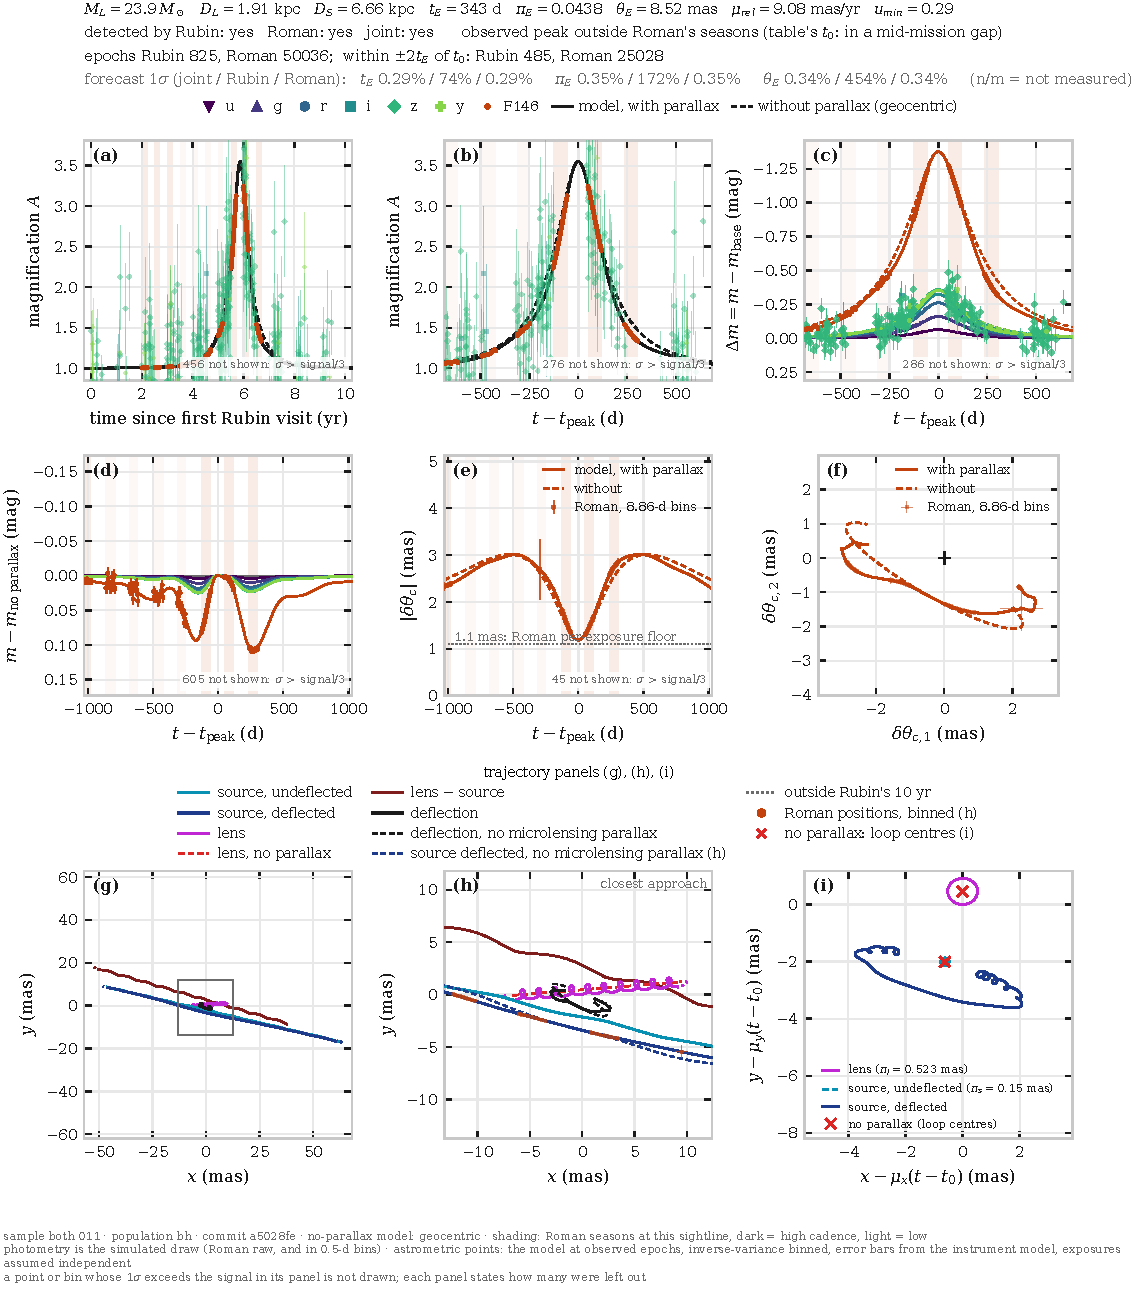
\includegraphics[width=.96\linewidth, trim=0 255 0 0, clip]{both_011_3x3}
\end{column}
\begin{column}{.32\linewidth}
\textbf{$23.9\,\Msun$ at $1.9$\,kpc}\\[3pt]
$\tE=343$\,d, $\tetE=8.5$\,mas
\vspace{6mm}

\uncover<2->{%
\begin{beamercolorbox}[rounded=true,sep=5pt,wd=\linewidth]{block body example}
Roman: \textbf{mass to $0.5\%$}\\[2pt]
Rubin alone: $\tE$ to $74\%$
\end{beamercolorbox}}
\end{column}
\end{columns}
\vfill
\refnote{This work, preliminary runs. Chosen for illustration, not typical.}
\note{\begin{itemize}
  \item Top row: photometry, Rubin's six bands and Roman's F146; Roman's seasons shaded (dark: high cadence).
  \item (d) the parallax signal; (e, f) the centroid shift (max.\ $3.0$\,mas) against Roman's $1.1$\,mas floor.
  \item Joint and Roman-alone precisions are the same here: $\tE$ to $0.3\%$, mass to $0.5\%$.
\end{itemize}}
\end{frame}

% !TeX root = ../seminar.tex
\section{Preliminary Results}

\begin{frame}{What the first overview forecast covers}
\begin{columns}[T]
\begin{column}{.47\linewidth}
\textbf{Three simulated lens populations}
\begin{itemize}
  \item Stellar population with remnants
  \item Isolated black holes, $3$--$1000\,\Msun$
  \item Neutron stars, near $1.35\,\Msun$
\end{itemize}
\end{column}
\begin{column}{.49\linewidth}
\textbf{September 2026 runs}
\begin{itemize}
  \item $1{,}829$ sightlines over $68$\,deg$^2$
  \item Six circles for Roman, $1.47$\,deg$^2$
  \item A ten-year observing window
\end{itemize}
\end{column}
\end{columns}
\vspace{4mm}
\uncover<2->{%
\begin{beamercolorbox}[rounded=true,sep=6pt,wd=\linewidth]{block body}
\textbf{How the forecasts are reported}\par
We weight draws by event rate. Headline yields apply a dust adjustment after simulation.
For a compact-object abundance $F$, the event yield scales as $N(F)=F\,N_1$.
\end{beamercolorbox}}
\vfill
\refnote{First overview report and proposal. Yields use the per-resolved-object counting convention.}
\note{The ordinary-lens run uses a Kroupa initial mass function evolved for an old bulge. The separate black-hole
      run samples $dN/dM\propto M^{-1}$ and uses a simple kinematic model. The neutron-star distribution
      is centred on $1.35\,\Msun$ with width $0.15\,\Msun$. $F$ is the fraction of Galactic stellar mass
      assigned to the compact-object population. In September, extinction near the plane was diagnosed
      as too low. The headline yields reweight outcomes using expected losses at fainter magnitudes,
      with a reference dust map checked against the near-infrared VVV survey. The simulations themselves
      were left as run. The backups give the details and the external checks.}
\end{frame}

\begin{frame}{Roman detects more events within its footprint}
\begin{columns}[c]
\begin{column}{.48\linewidth}
\textbf{Ordinary lenses inside Roman's fields}\\[4pt]
\begin{tabular}{@{}lr@{}}
Roman detections & $\approx50{,}000$ \\
Rubin detections & $\approx4{,}900$
\end{tabular}
\vspace{6mm}

\uncover<2->{Outside those fields, Rubin accounts for \textbf{about 60\% of the detections across the simulated region}.}
\end{column}
\begin{column}{.47\linewidth}
\centering
\textbf{Extinction toward the bulge}\\[-1mm]
{\small At $A_V\approx7.2$ magnitudes}
\begin{tikzpicture}[font=\small]
  \fill[orange!65] (0,1.6) rectangle (5.18,2.1);
  \node[anchor=west, font=\footnotesize] at (0.1,1.85) {Rubin $r$: $6.1$\,mag};
  \fill[jdblue!65] (0,0.8) rectangle (1.19,1.3);
  \node[anchor=west, font=\footnotesize] at (1.3,1.05) {Roman F146: $1.4$\,mag};
  \draw (0,0.6) -- (0,2.25);
\end{tikzpicture}
\end{column}
\end{columns}
\vfill
\refnote{Rate-weighted, dust-adjusted yields for the ten-year window. Extinction law: \ads{1989ApJ...345..245C}{Cardelli et al.\ 1989}.}
\note{The two detection counts overlap. For ordinary lenses the report gives $50{,}350\pm2{,}945$
      for Roman and $4{,}853\pm515$ for Rubin within the footprint. Of all ordinary-lens detections
      in the simulated region, $(59\pm5)\%$ are outside Roman's footprint, where Rubin is the only
      simulated observer. The bar chart takes $A_V$ from the median toward Roman's footprint detections.
      Within the footprint, nearly all Rubin-only ordinary-lens detections peak when Roman is not observing.
      Rubin's time coverage matters most when the signal is concentrated inside a Roman gap.}
\end{frame}

\begin{frame}{Roman's data sharpen masses for events Rubin detects}
\centering
\textbf{Rubin detections inside Roman's fields}\\[3pt]
{\small Rubin data alone $\longrightarrow$ Rubin and Roman data combined}\\[3mm]
\renewcommand{\arraystretch}{1.2}
\begin{tabular}{lccc}
\toprule
 & ordinary lenses & neutron stars & black holes \\
\midrule
$\tE$ and $\piE$ above $2\sigma$ & $5\%\to28\%$ & $5\%\to37\%$ & $12\%\to83\%$ \\
\rowcolor{jdlightestblue}
mass error below $10\%$ & $\approx0\to8\%$ & $\approx0\to16\%$ & $0.2\%\to\mathbf{53\%}$ \\
\bottomrule
\end{tabular}

\vspace{4mm}
\uncover<2->{\small About \textbf{13\% more} black-hole masses reach $10\%$ in the joint forecast across the full footprint,
compared with the Roman-only yield.\par}
\vfill
\refnote{Rate-weighted and dust-adjusted. Underlying Rubin detections before dust adjustment have
$\Neff=685$ (ordinary), $1{,}687$ (neutron stars), and $2{,}011$ (black holes).}
\note{The table has a common denominator across each pair of fractions. The reverse comparison below it
      compares two total footprint yields, about $651F$ joint and $579F$ Roman-only for black holes.
      A $10\%$ mass means a forecast fractional $1\sigma$ error below $0.10$. The joint black-hole share
      in the table is $53.3\pm1.8$ percent. Most Rubin black-hole detections in these fields are also
      Roman detections. Rubin broadens both sky and time coverage, but extra visits often have little
      information on well-covered, heavily extinguished events.}
\end{frame}

\begin{frame}{For black holes, parallax limits the mass precision}
\begin{columns}[c]
\begin{column}{.52\linewidth}
\centering\small
\textbf{Roman precision in the September runs}
\begin{tikzpicture}[x=.046cm,y=.92cm,font=\footnotesize]
  \node[anchor=east] at (-3,2.3) {$\tetE$};
  \node[anchor=east] at (-3,1.3) {$\piE$};
  \node[anchor=east] at (-3,.3) {$\Ml$};
  \foreach \y/\val/\lab in {2.3/97/97,1.3/12.85/13,.3/12.6/13} {
    \fill[jdverylightgrey] (0,\y-.22) rectangle (100,\y+.22);
    \fill[jdblue!75] (0,\y-.22) rectangle (\val,\y+.22);
    \node[anchor=east] at (99,\y+.43) {$\lab\%$};
  }
\end{tikzpicture}\\[-1mm]
{\footnotesize Share with forecast error below $10\%$}
\end{column}
\begin{column}{.42\linewidth}
Roman's detections have a median maximum centroid shift of \textbf{$3.4$\,mas}.

\vspace{4mm}
\uncover<2->{The Earth--L2 baseline gives negligible median gain in black-hole parallax precision in the paired simulation.}
\end{column}
\end{columns}
\vfill
\refnote{Rate-weighted, as simulated. Each bar uses the Roman sample with a forecast available
for that parameter ($\Neff\simeq8{,}700$).}
\note{The rates shown here come from the report's compact-object table. The Roman-only mass
      fraction after the separate dust adjustment is about $10\%$ of Roman's detections.
      For the black-hole parallax test, rerun the precision calculation with Roman placed at Earth
      and keep the sampling and noise fixed. The median parallax-error ratio for L2 vs Earth was
      effectively one for black holes. The projected baseline is short, and the annual signal already
      contributes information across Roman's observing seasons.}
\end{frame}

\begin{frame}{How many black holes could Roman weigh?}
\centering
For a black-hole population containing \textbf{$0.5$--$3\%$} of Galactic stellar mass
\vspace{4mm}

\begin{columns}[T]
\begin{column}{.43\linewidth}
\begin{beamercolorbox}[rounded=true,sep=8pt,wd=\linewidth]{block body}
\centering{\Large\bfseries 30--170}\\[2pt]
black-hole events detected
\end{beamercolorbox}
\end{column}
\begin{column}{.43\linewidth}
\begin{beamercolorbox}[rounded=true,sep=8pt,wd=\linewidth]{block body example}
\centering{\Large\bfseries 3--17}\\[2pt]
masses with errors below $10\%$
\end{beamercolorbox}
\end{column}
\end{columns}
\vspace{4mm}

$\displaystyle N_{\rm det}=(5{,}660\pm320)F,\qquad N_{\rm mass}=(579\pm42)F$
\vspace{3mm}

\uncover<2->{\small Dust, field geometry, correlated astrometric errors and the assumed black-hole population all affect these yields.\par}
\vfill
\refnote{First overview report, after the dust adjustment. Roman-only forecast in the $1.47$\,deg$^2$
model footprint within the ten-year survey window.}
\note{The endpoints vary the assumed $F$ with the mass function and kinematics held fixed. They are an abundance
      scenario range. The uncertainties on the coefficients include Monte Carlo error and uncertainty
      in the dust adjustment. They do not include all survey and population-model uncertainties.
      An astrometric floor that is correlated across visits especially affects weaker centroid signals.
      The numerical yields here use the original model footprint, so the proposal includes a rerun on the adopted fields.}
\end{frame}

% !TeX root = ../seminar.tex
\begin{frame}{What comes next in the thesis}
\begin{itemize}\setlength{\itemsep}{9pt}
  \item<+-> \textbf{Refine the forecast.} Run on the adopted Roman footprint at finer resolution
        and test how correlated astrometric errors affect mass precision.
  \item<+-> \textbf{Test black-hole populations.} Vary the mass distribution and the velocities
        black holes receive at birth.
  \item<+-> \textbf{Infer the population.} Use mock detections, with survey selection and mass
        errors, to test what we can learn about abundance and a possible low-mass gap.
\end{itemize}
\note{The first task is to establish which forecast results are stable as we refine the sky grid
      and vary the astrometric noise assumptions. The second asks how the predicted observations
      change with different black-hole populations. The third applies those forecasts to inference
      from a realistically selected catalogue.}
\end{frame}

% !TeX root = ../seminar.tex
\section{Summary}

\begin{frame}{Summary}
\begin{itemize}
  \item<+-> $\sim\!10^8$ stellar black holes in the Galaxy, \textbf{one} isolated one weighed. Microlensing weighs
        them: photometry gives $\piE$, astrometry gives $\tetE$, and $\Ml=\tetE/\kappa\piE$
  \item<+-> A two-telescope simulator forecasts Rubin, Roman and their combination \textbf{on the same events}
  \item<+-> In its fields \textbf{Roman dominates} (the dust); Roman turns Rubin's detections into measurements
        (black-hole masses: $\approx0\to\sim\!50\%$); Rubin owns the wide sky
  \item<+-> Black holes: $\tetE$ is easy for Roman, the \textbf{parallax} is the limit;
        $\sim\!30$--$170$ events and $3$--$17$ masses to $10\%$ for $F_{\rm BH}=0.005$--$0.03$
  \item<+-> Next: a better model (dust, Roman's errors, black-hole physics) $\to$ the full run $\to$
        Bayesian fits and image resolution $\to$ \textbf{the black-hole mass function and the mass gap}
\end{itemize}
\end{frame}

{
\usebackgroundtemplate{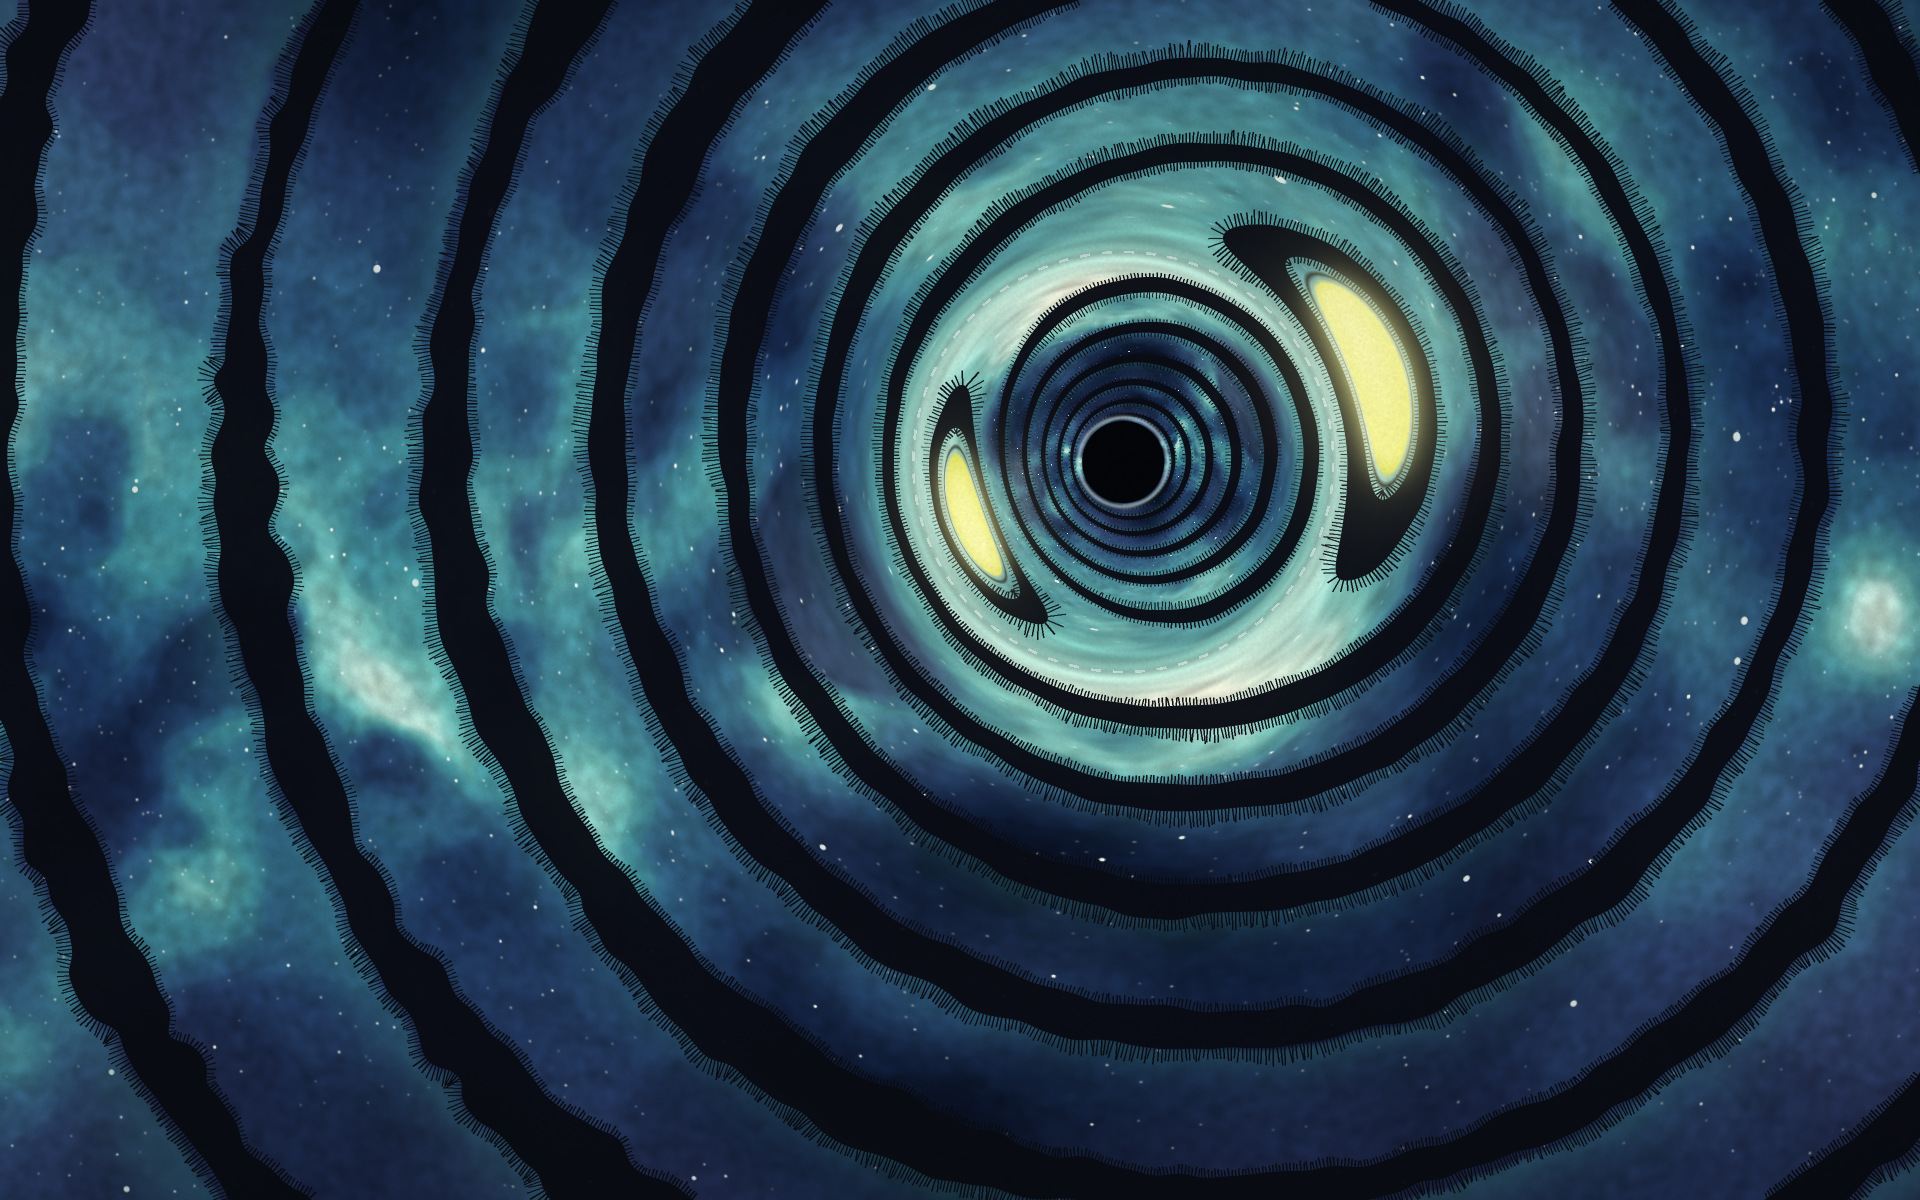
\includegraphics[width=\paperwidth,height=\paperheight]{microlensing-cartoon}}
\begin{frame}[plain]
\begin{center}
\vspace*{6.9cm}
\contourlength{2pt}
\contournumber{20}
\contour{black}{\Huge \textcolor{white}{Thank you for your attention!}}\\
\end{center}
\end{frame}
}


\appendix
% !TeX root = ../seminar.tex
% Backup slides: not counted in the frame numbers (appendixnumberbeamer).
\section*{Backup}

\begin{frame}[plain]
\vfill
\centering
{\usebeamerfont{title}\usebeamercolor[fg]{title}\Large Backup slides}
\vfill
\end{frame}

\begin{frame}{Backup: what goes into a mass forecast?}
For small, jointly estimated uncertainties, propagate the covariance in the two fitted scales:
\[
 \sigma^2(\ln \Ml)=\sigma^2(\ln\tetE)+\sigma^2(\ln\piE)
       -2\,\mathrm{cov}(\ln\tetE,\ln\piE).
\]
\begin{itemize}
  \item The first overview forecast used separate photometric and astrometric Fisher blocks,
        with the mass error calculated from fractional errors in quadrature.
  \item In a real fit, the baseline includes source position, proper motion and source parallax.
        Neighbouring light can shift the reference centroid as the source brightens.
  \item Fisher errors describe the local curvature near the simulated parameters.
        Sparse coverage can leave disconnected solutions that require fits to explore.
\end{itemize}
\refnote{First overview report, sections on mass inference and Fisher forecasts.}
\note{In the full model, for an angular source radius $\theta_\star$ inferred independently, a detectable
      finite-source signature can also constrain $\rho=\theta_\star/\tetE$ and hence $\tetE$.
      The September headline analysis used a point source.}
\end{frame}

\begin{frame}{Backup: a compact-object precision cross-check}
\centering
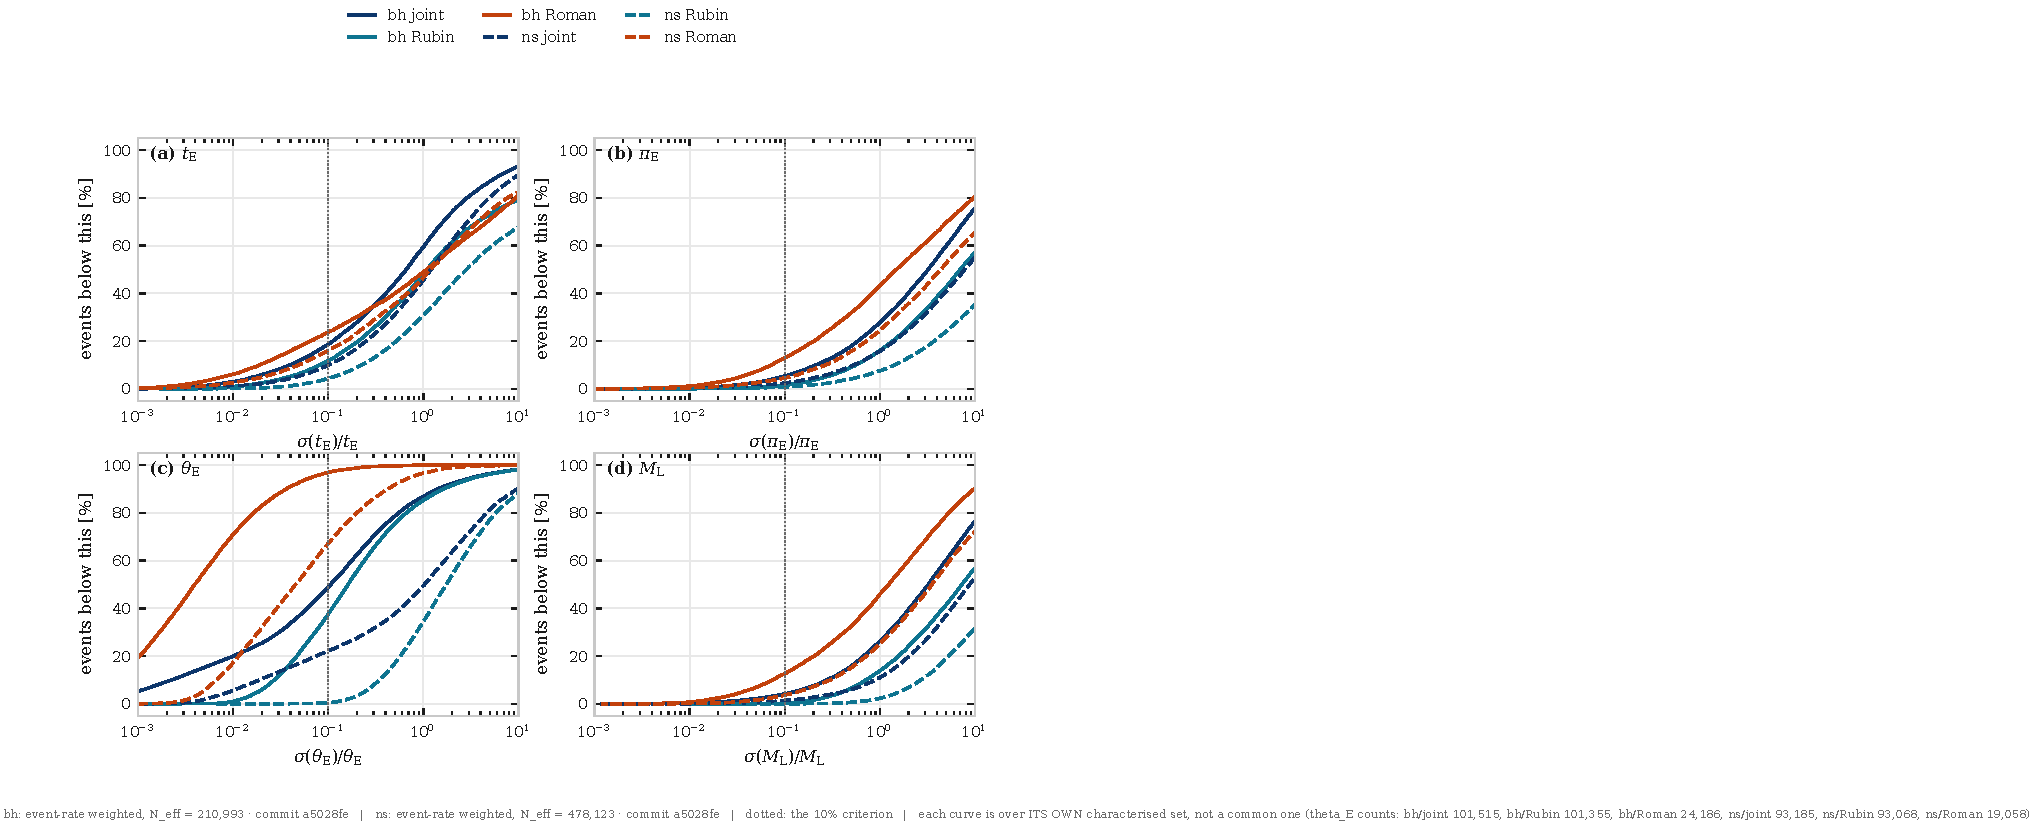
\includegraphics[height=.60\paperheight, trim=0 14 508 0, clip]{p7_precision}\\[2pt]
\refnote{September simulations. Event-rate-weighted cumulative fractional errors. Each curve uses
its own survey and parameter sample. Compare precision gains on a common set of events.}
\note{For the Roman black-hole forecasts the effective sample size is about $8{,}700$. The
      effective sample sizes printed inside the original plot refer to all draws in each population,
      so they should not be used as the sample size of a selected curve.}
\end{frame}

\begin{frame}{Backup: the astrometric signal scale}
\vspace{1mm}
\begin{columns}[c]
\begin{column}{.56\linewidth}
\centering
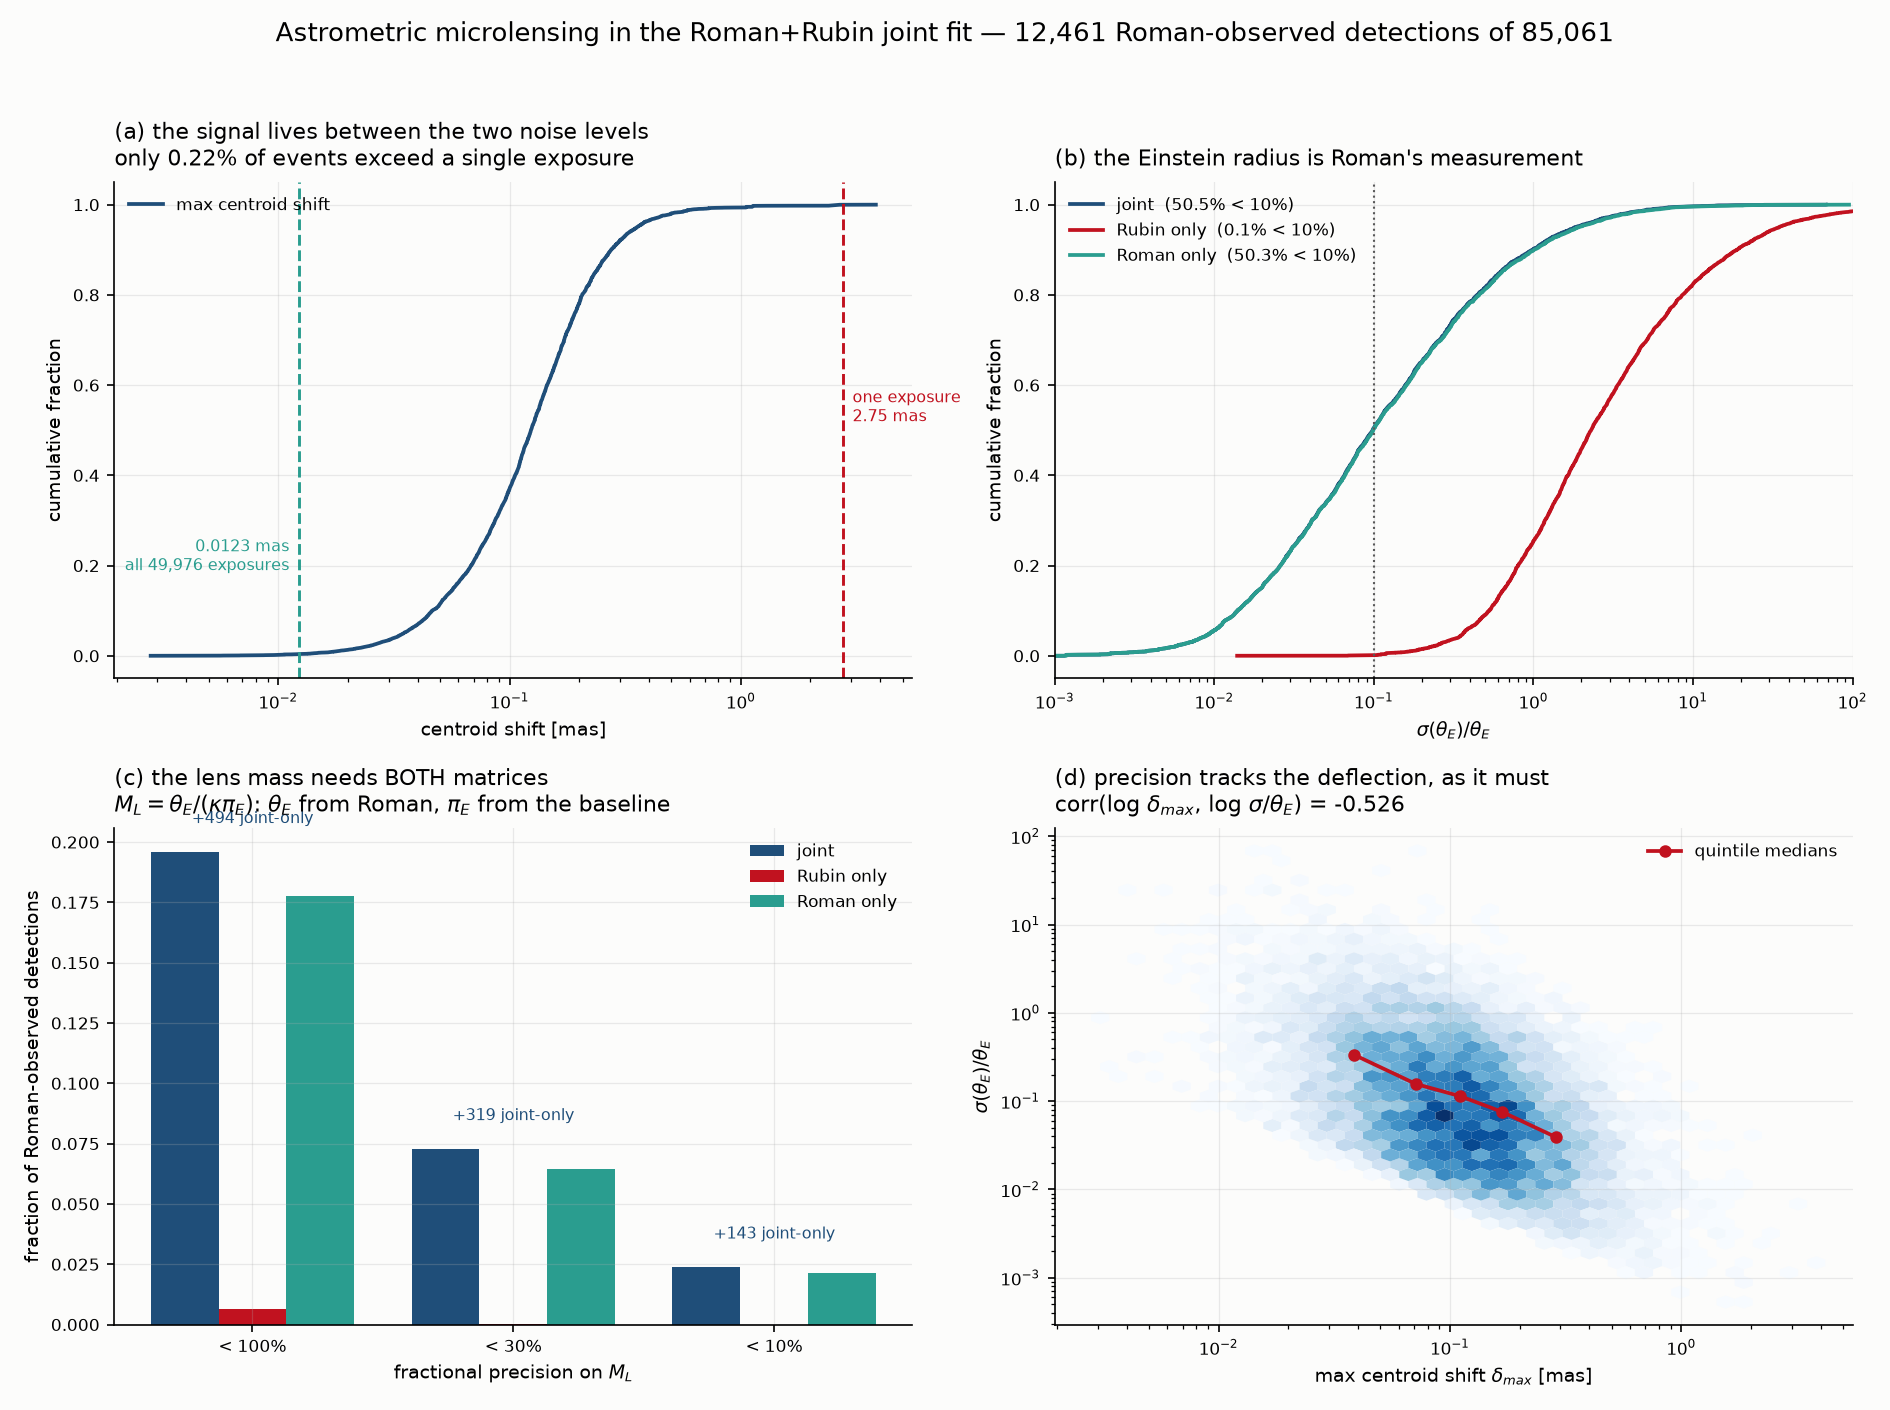
\includegraphics[width=.94\linewidth]{h5_astrometry_summary}\\[1mm]
\refnote{Ordinary lenses in Roman's fields, as simulated.}
\end{column}
\begin{column}{.40\linewidth}
\begin{itemize}\setlength{\itemsep}{6pt}
  \item \textbf{Black holes}: $3.4$\,mas median maximum shift in Roman detections
  \item \textbf{Ordinary lenses}: $0.12$\,mas; the forecast relies on repeated exposures
  \item Rubin adds little to Roman's typical $\tetE$ forecast
\end{itemize}
\vspace{4mm}
{%
\begin{beamercolorbox}[rounded=true,sep=5pt,wd=\linewidth]{block body alerted}
\centering Risk: does the $1.1$\,mas floor average down?
\end{beamercolorbox}}
\end{column}
\end{columns}
\vfill
\refnote{Astrometric floor: \ads{2019JATIS...5d4005S}{Sanderson et al.\ 2019}}
\note{\begin{itemize}
  \item The $1.1$\,mas bright-source floor in the first overview is a model input. Actual visit errors
        depend on source brightness, and high-cadence visits need not be independent.
  \item The listed medians are after the dust adjustment. Their underlying Roman detection samples had
        $\Neff$ of about $8{,}600$ (black holes) and $3{,}700$ (ordinary lenses) before the adjustment.
  \item An event's maximum centroid shift and the error on its fitted Einstein radius are different
        quantities. Joint time coverage and modelling the unlensed track also matter.
\end{itemize}}
\end{frame}

\begin{frame}{Backup: seeing the two images}
\vspace{1mm}
\begin{columns}[c]
\begin{column}{.56\linewidth}
\centering
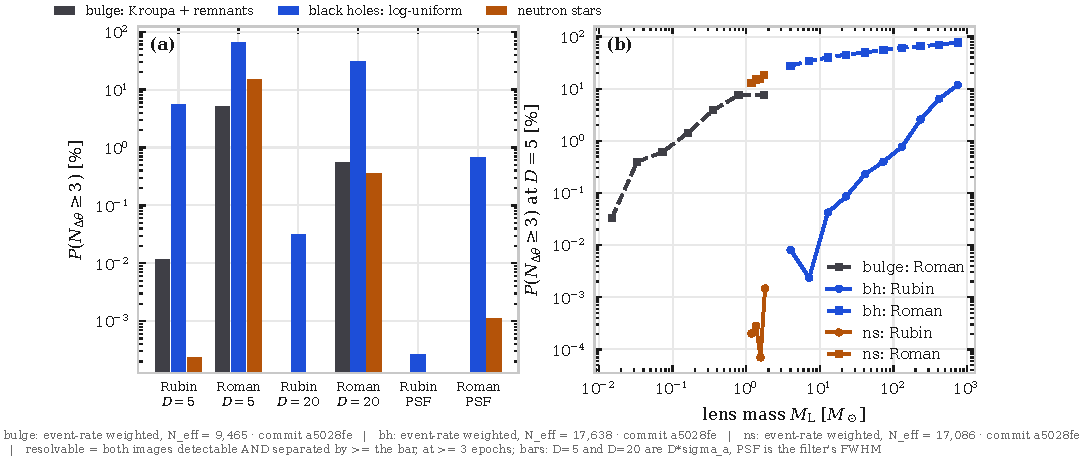
\includegraphics[width=.94\linewidth]{p6_resolution}\\[1mm]
\refnote{(a) by population, telescope and criterion; (b) against lens mass. Figure as simulated.}
\end{column}
\begin{column}{.40\linewidth}
\[
  \Delta\theta = \tetE\sqrt{u^2+4}
\]
{Roman black-hole detections,\\ dust-adjusted:\\[3pt]
\begin{tabular}{@{}ll@{}}
generous bar & $34\%$ \\
strict bar & $15\%$ \\
PSF width & $0.25\%$
\end{tabular}}
\vspace{5mm}

{%
\begin{beamercolorbox}[rounded=true,sep=5pt,wd=\linewidth]{block body alerted}
\centering Simulated Roman images can test which thresholds are realistic.
\end{beamercolorbox}}
\end{column}
\end{columns}
\vfill
\refnote{Criterion: \ads{2026ApJ..1009..116S}{Sajadian \& Makler 2026, ApJ 1009, 116}}
\note{\begin{itemize}
  \item Resolvable: at least three visits with both images detectable and $\Delta\theta$ above a bar:
        $\mathcal{D}\sigma_{\rm ast}$ with $\mathcal{D}=5$ (generous) or $20$ (strict), or the PSF width.
  \item Rubin resolves $\approx5\%$ of its black-hole events at the generous bar; for lighter lenses resolution is rare.
  \item The predicted fractions span two orders of magnitude. The criterion for Roman's diffraction-limited images must be
        measured on simulated Roman images.
\end{itemize}}
\end{frame}

\begin{frame}{Backup: a central transit of an extended star}
\centering
\vspace{2mm}
\animategraphics[autoplay, loop, controls=off, poster=31, width=.76\linewidth]{16}{img/anim/frame_}{00}{80}

\vspace{4mm}
A ring appears at exact centre alignment in this example.\\ Most events pass well outside the source disc.
\vfill
\refnote{Reverse ray tracing of a limb-darkened star, $\theta_\star=0.6\,\tetE$ (A.~Salehi); the curves are
measured from the traced images.}
\note{\begin{itemize}
  \item In a real event the images are too close to separate: a telescope sees only their total light and its centre.
  \item At exact centre alignment the ring is symmetric. During the transit the finite source caps the
        magnification and reverses the centroid shift. Dashed grey: a point source.
\end{itemize}}
\end{frame}

\begin{frame}{Backup: light curves and centroid shifts for several $u_0$}
\centering
\vspace{2mm}
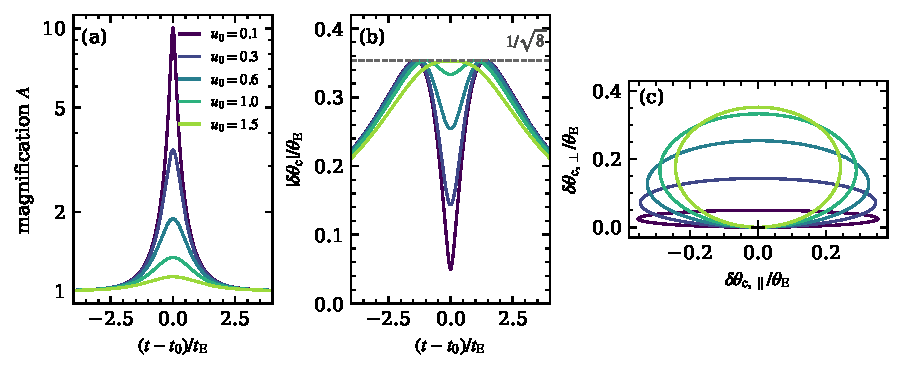
\includegraphics[width=.86\linewidth]{theory_curves}\\[3mm]

\small (a) magnification, (b) centroid shift against time, (c) the centroid's ellipse on the sky.
\end{frame}

\begin{frame}{Backup: gap filling --- when Rubin matters inside Roman's fields}
\begin{columns}[T]
\begin{column}{.56\linewidth}
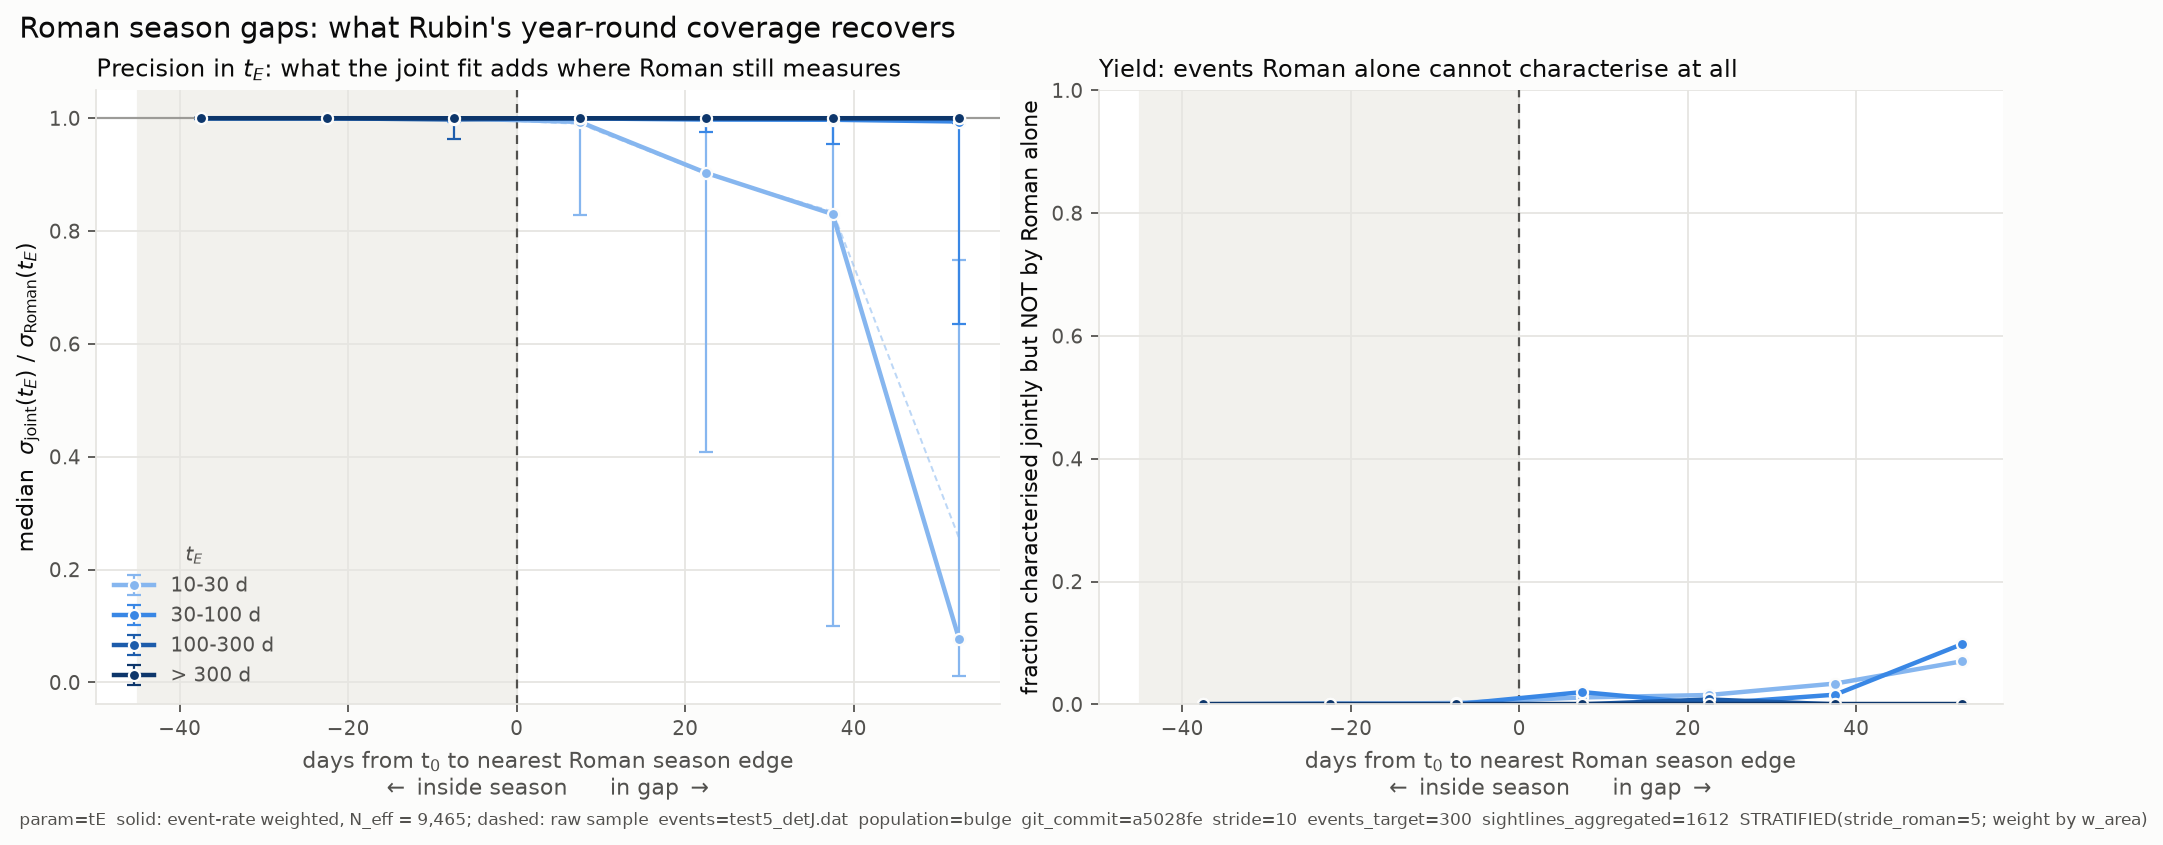
\includegraphics[width=\linewidth]{f2_gap_filling}
\refnote{Left: median $\sigma_{\rm joint}(\tE)/\sigma_{\rm Roman}(\tE)$ against the peak's distance from a season edge,
per $\tE$ bin. Right: fraction characterised jointly but not by Roman. Shaded: inside a season.}
\end{column}
\begin{column}{.42\linewidth}
\footnotesize
$10$--$30$\,d events, by where the peak falls:\\[2pt]
\begin{tabular}{@{}lcc@{}}
\toprule
peak & $\dfrac{\sigma_{\rm joint}}{\sigma_{\rm Roman}}(\tE)$ & $\Neff$ \\
\midrule
anywhere in a gap & $0.97$ & $670$ \\
$>15$\,d past an edge & $0.83$ & $376$ \\
$>30$\,d past & $0.44$ & $177$ \\
$>45$\,d past & $\mathbf{0.08}$ & $62$ \\
in a season & $1.00$ & $888$ \\
\bottomrule
\end{tabular}
\begin{itemize}
  \item Roman itself detects $96\%$ of in-gap events, from the wings
  \item The gain is largest for short events deep in a gap
  \item As simulated, without the later dust adjustment
\end{itemize}
\end{column}
\end{columns}
\end{frame}

\begin{frame}{Backup: two parallax baselines}
\begin{columns}[T]
\begin{column}{.52\linewidth}
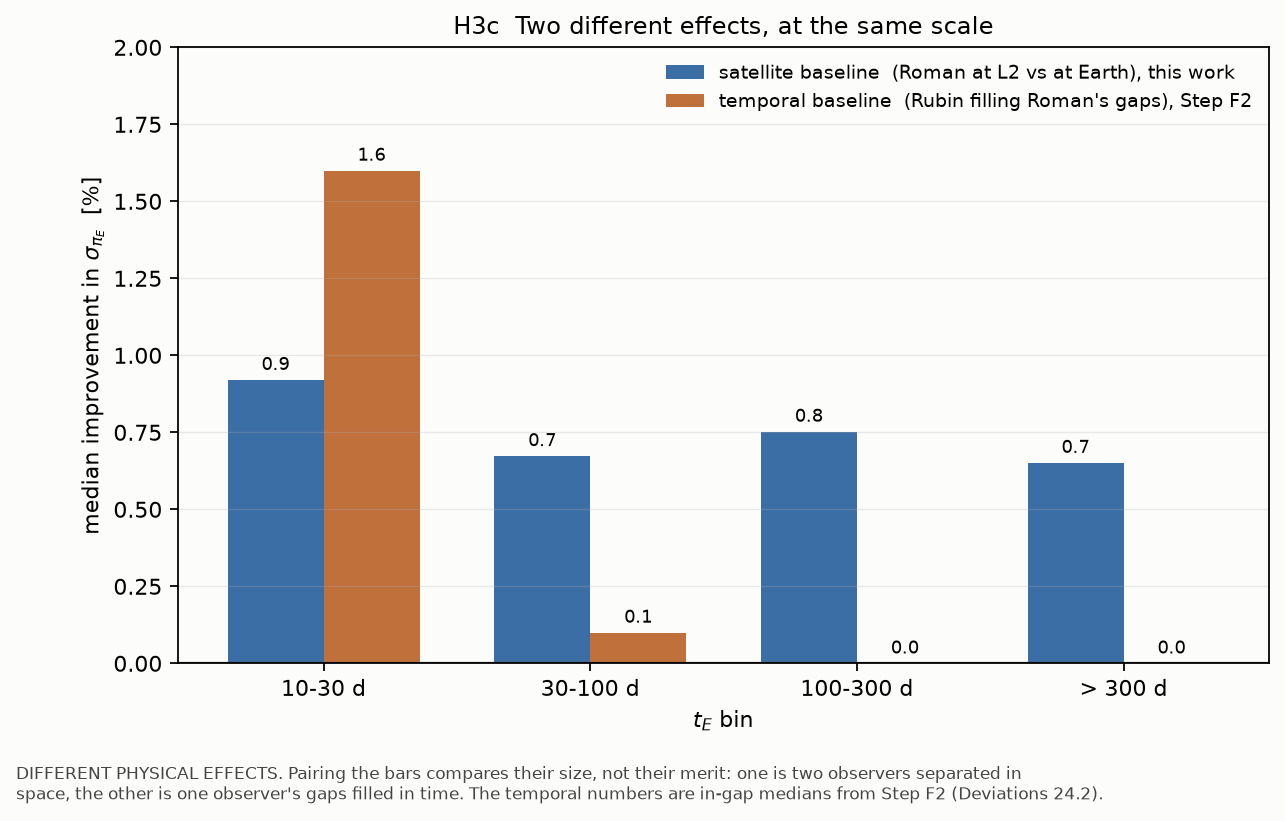
\includegraphics[width=\linewidth]{h3c_honest}
\refnote{Median improvement in $\sigma(\piE)$ per $\tE$ bin. Blue: Roman at L2 vs Roman at Earth (spatial).
Orange: joint vs Roman for events peaking in a gap (temporal).}
\end{column}
\begin{column}{.46\linewidth}
\small
\textbf{Spatial} (L2 vs Earth, $0.01$\,AU): each event forecast twice
\begin{itemize}\footnotesize
  \item Ordinary lenses: median error ratio $0.991$ ($\Neff=3{,}521$); $92\%$ improve
  \item $1.2\%$ improve by $>2\times$: short ($\tE\approx5$\,d), high-magnification events
  \item black holes and neutron stars: median ratio near one
\end{itemize}
\textbf{Temporal} (Rubin while Roman is not observing)
\begin{itemize}\footnotesize
  \item $10$--$30$\,d events: $1.6\%$ vs $0.9\%$ spatial
  \item large only for events wholly inside a gap
\end{itemize}
\end{column}
\end{columns}
\note{These ratios are conditional on the September orbit and noise models. The later orbit audit
      documented a bias in the legacy projection of Earth's orbit toward the bulge. The September
      median quantifies the paired test in that model. It is a historical forecast result.}
\end{frame}

\begin{frame}{Backup: what only the combination characterises}
\begin{columns}[T]
\begin{column}{.62\linewidth}
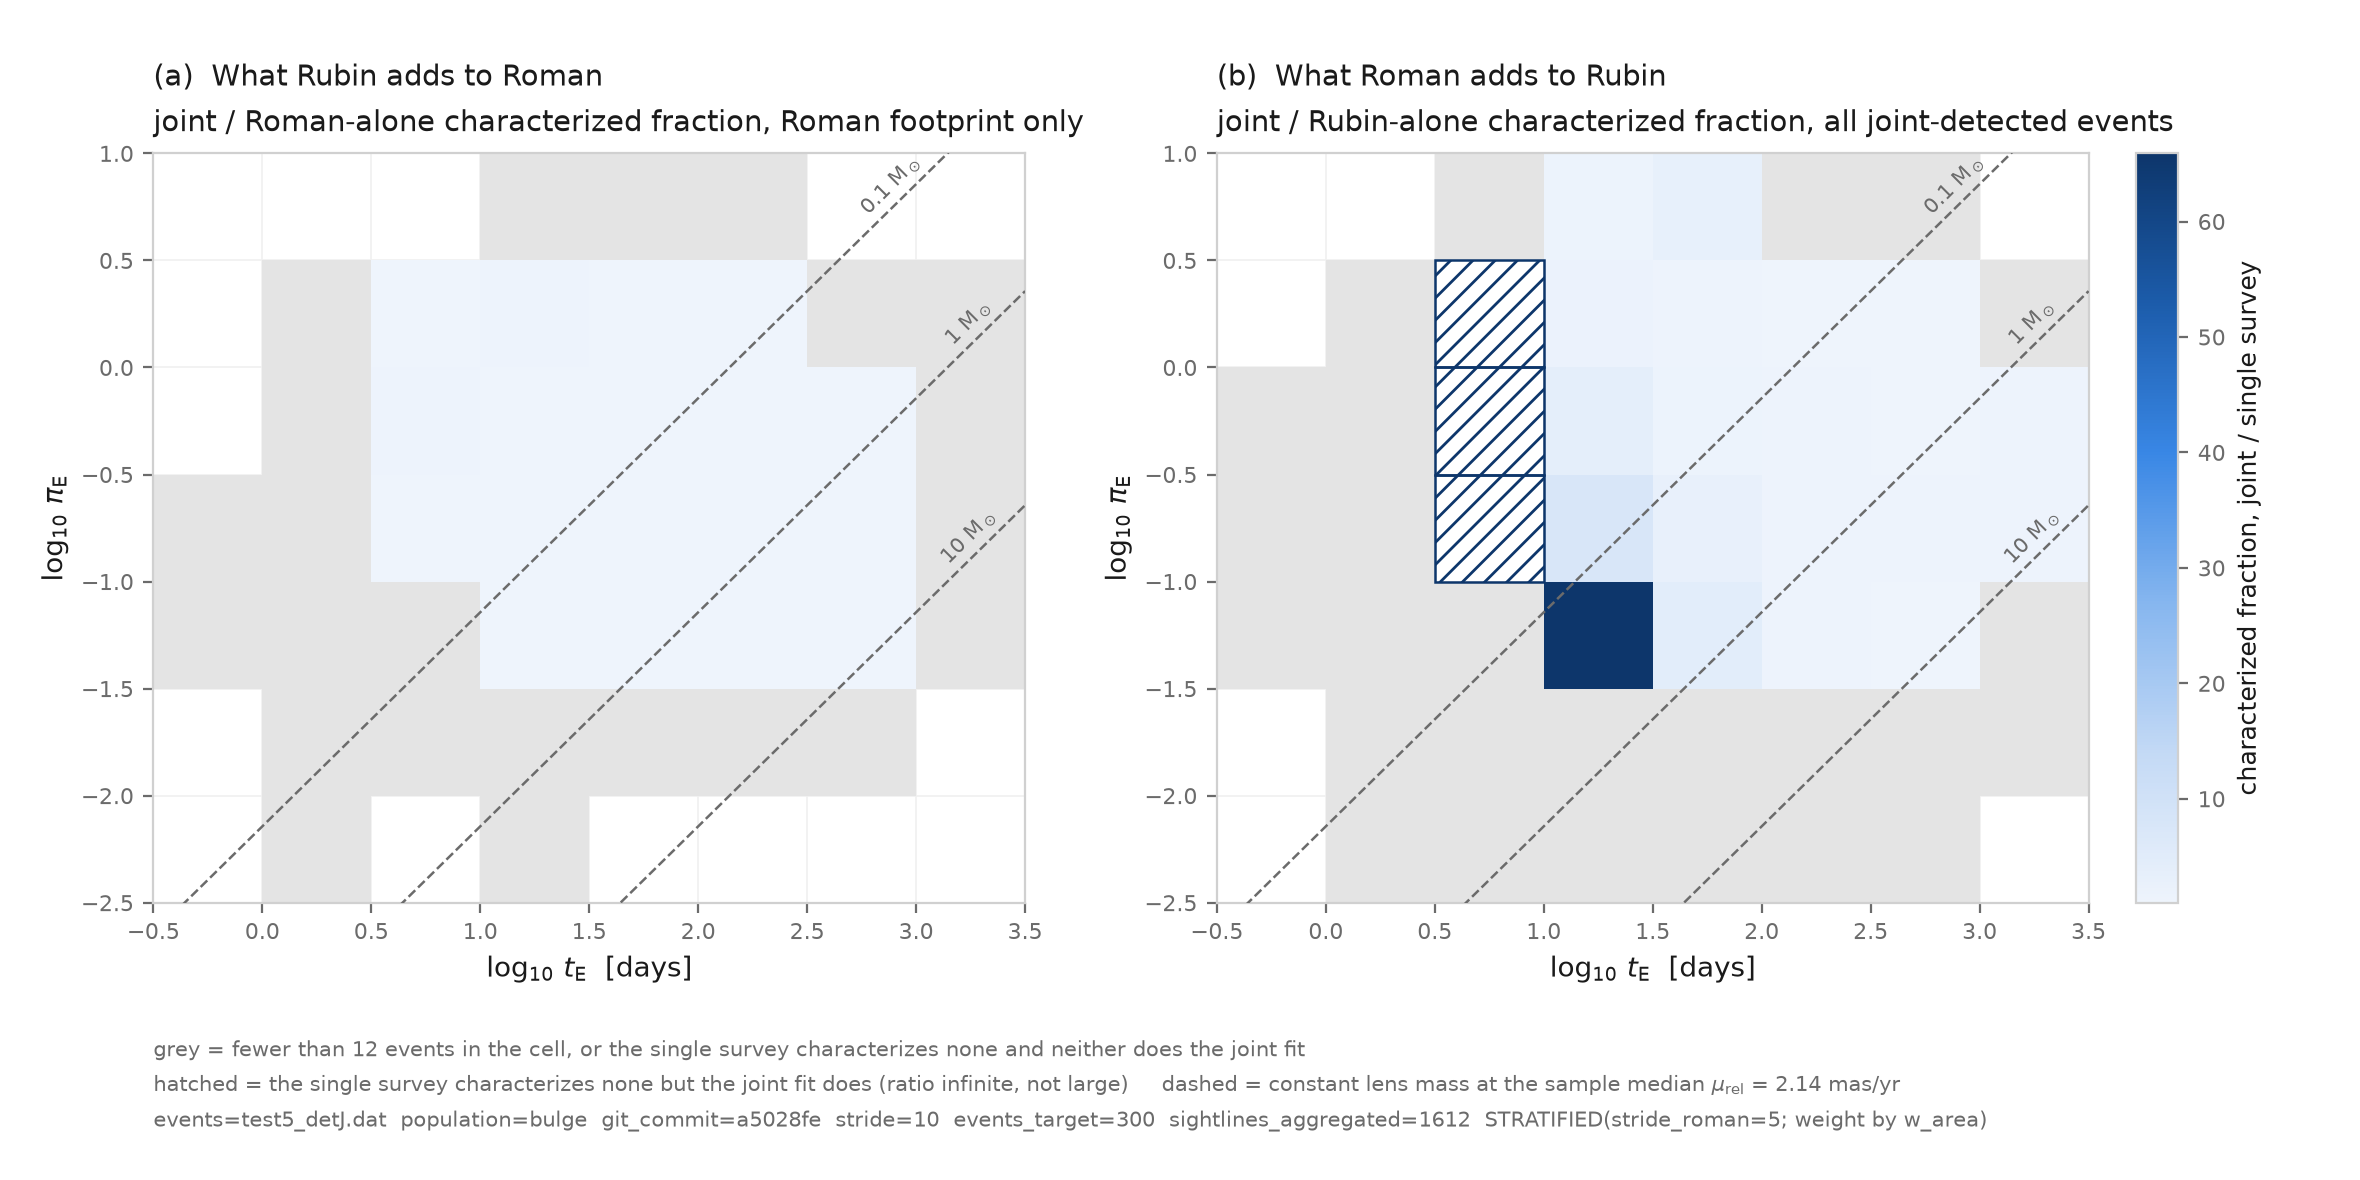
\includegraphics[width=\linewidth]{f3_characterization_map}
\refnote{Characterised fraction, joint over single survey, in the $(\tE,\piE)$ plane. (a) What Rubin adds to Roman;
(b) what Roman adds to Rubin (hatched: Rubin alone characterises none, the joint fit does). Dashed: constant mass.}
\end{column}
\begin{column}{.36\linewidth}
\small
\begin{itemize}
  \item (a) Adding Rubin changes the characterised sample little across most of this plane
  \item (b): Roman multiplies what Rubin can characterise, most for short events --- at $10$--$30$\,d and
        $\piE\sim0.03$--$0.1$, $66\times$
  \item $358$ of $12{,}461$ simulated footprint detections are characterised \emph{only} jointly: each survey holds part of the information
\end{itemize}
\end{column}
\end{columns}
\end{frame}

\begin{frame}{Backup: absolute precision, ordinary lenses}
\begin{columns}[T]
\begin{column}{.6\linewidth}
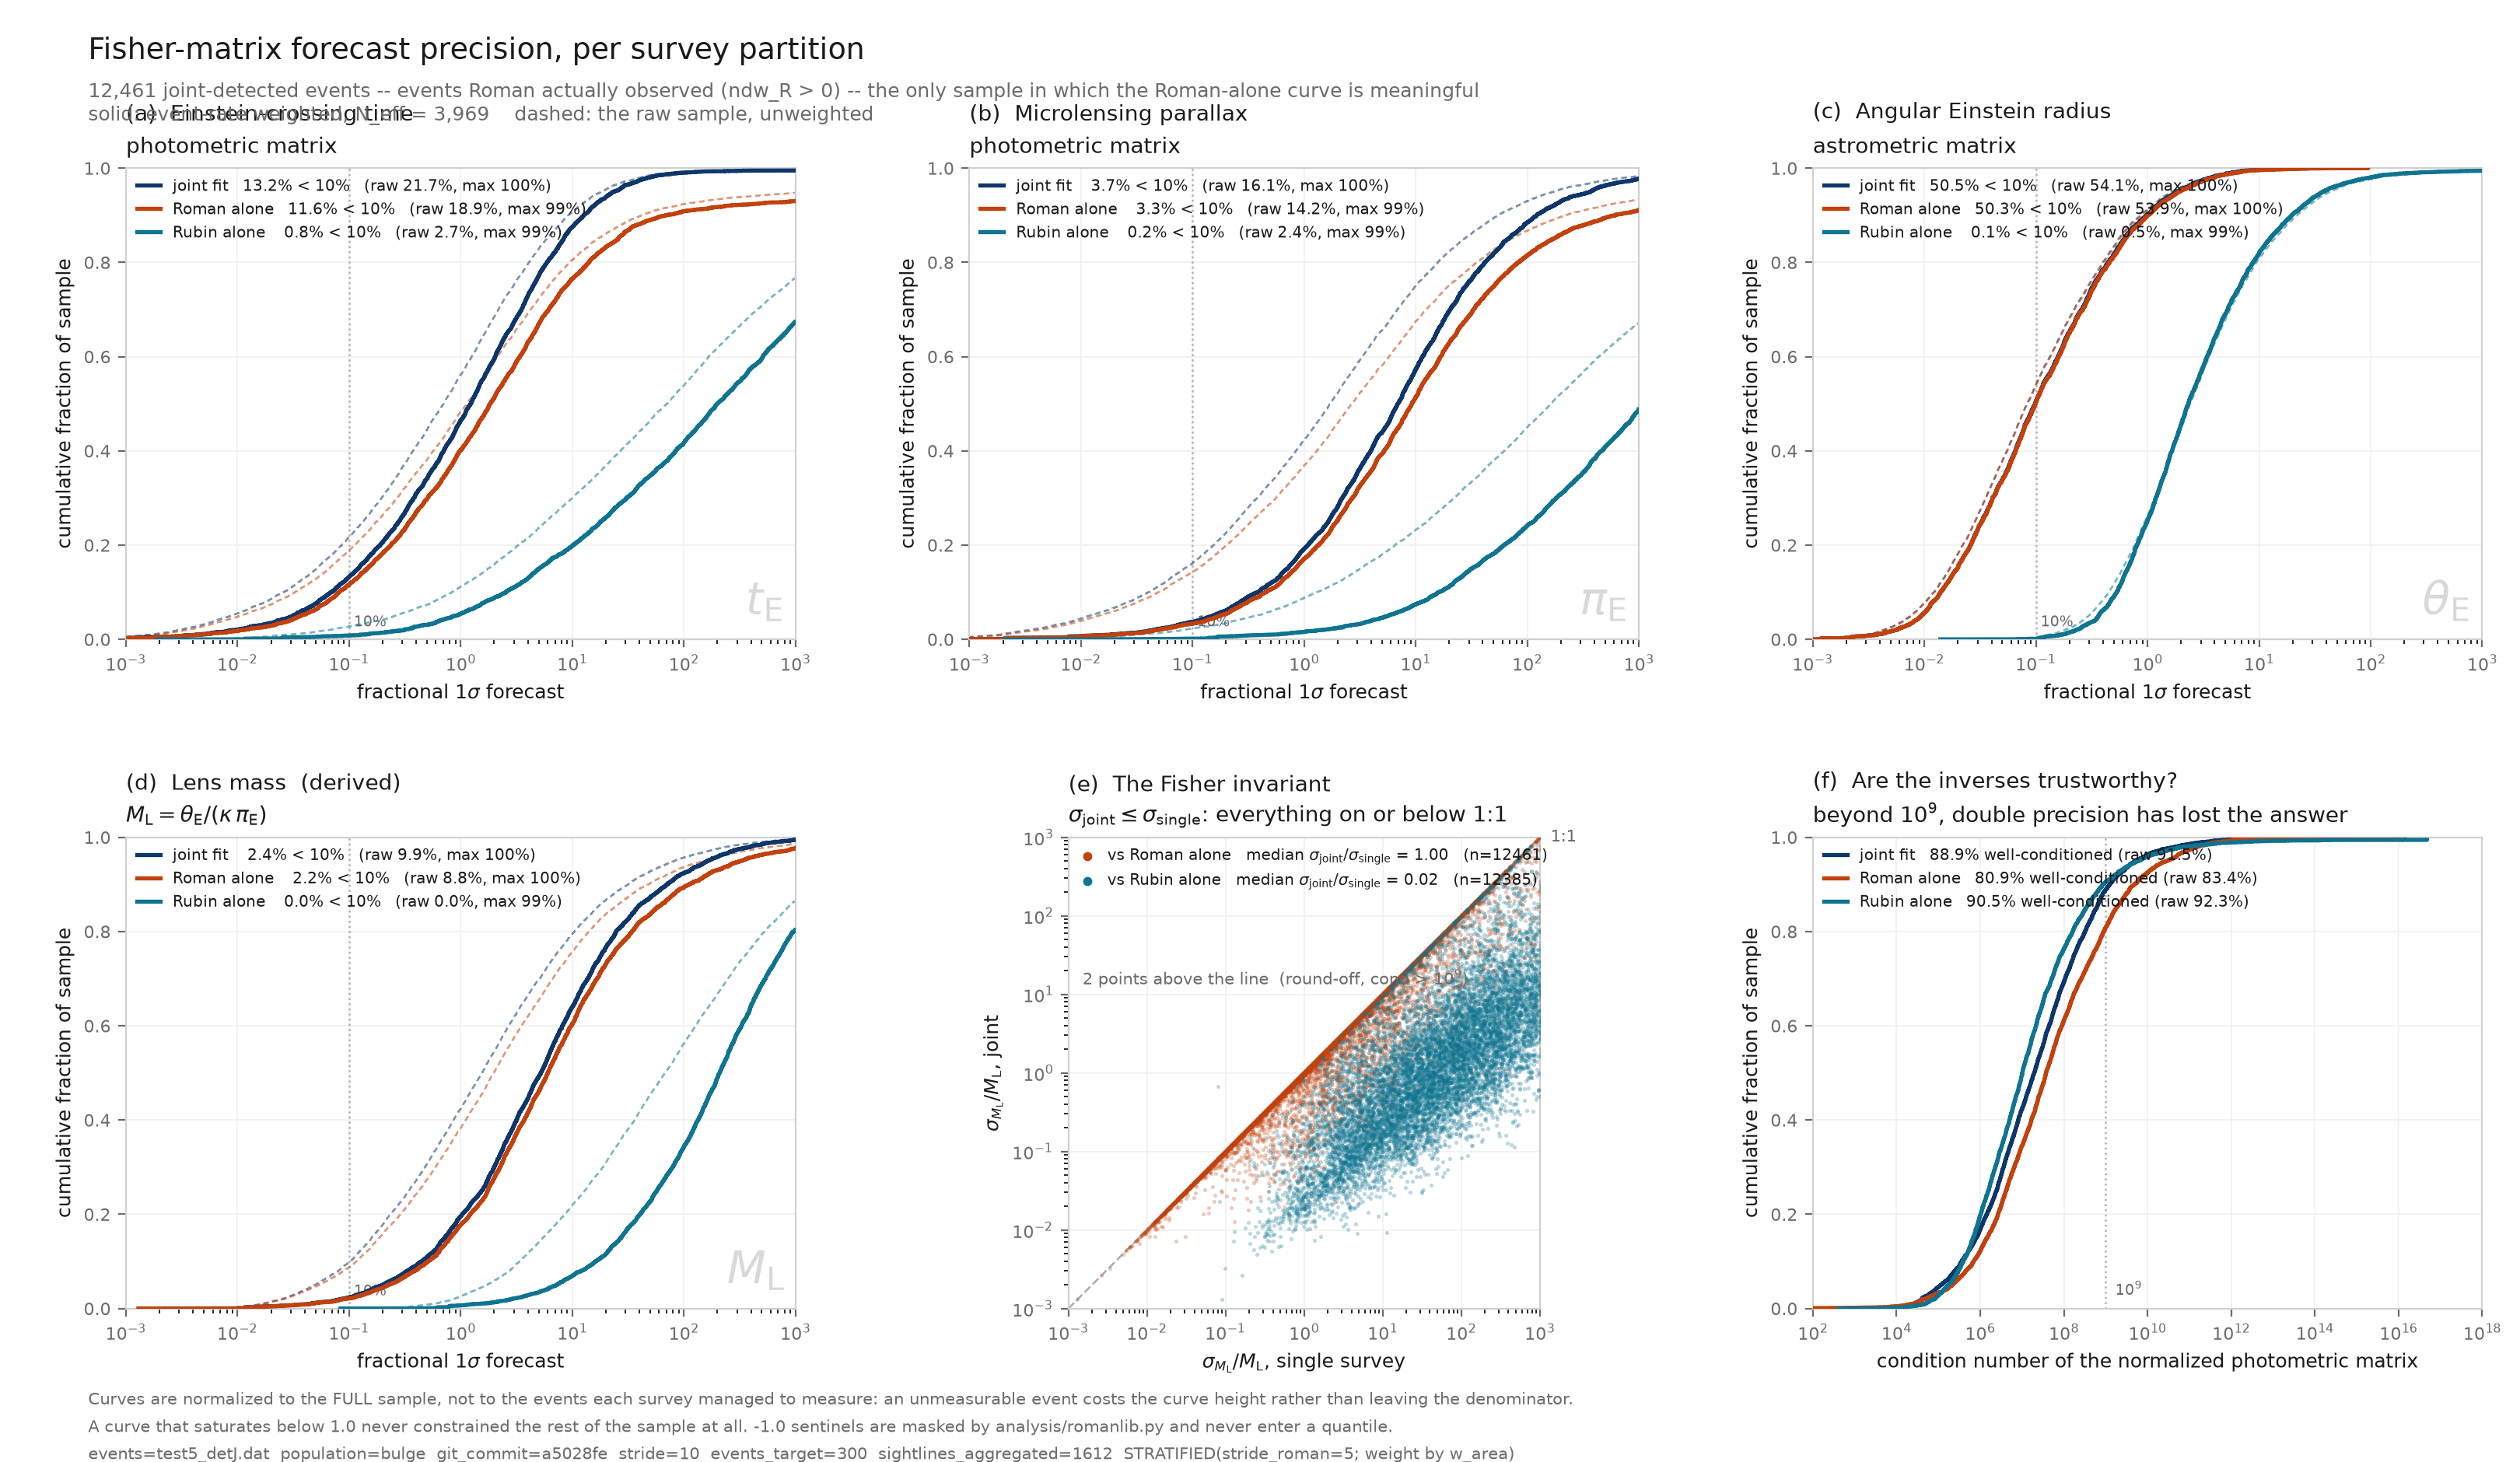
\includegraphics[width=\linewidth]{f4_fisher_precision}
\refnote{Fractional $1\sigma$ forecasts per survey over Roman's footprint detections ($\Neff\approx4{,}000$):
(a--c) fitted parameters, (d) mass, (e) $\sigma_{\rm joint}\le\sigma_{\rm single}$ event by event, (f) condition numbers.}
\end{column}
\begin{column}{.38\linewidth}
\small
Weighted \% measured to $10\%$ (as simulated):\\[3pt]
\begin{tabular}{@{}lccc@{}}
\toprule
 & joint & Roman & Rubin \\
\midrule
$\tE$ & $13.2$ & $11.6$ & $0.8$ \\
$\piE$ & $3.7$ & $3.3$ & $0.15$ \\
$\tetE$ & $50.5$ & $50.3$ & $0.13$ \\
$\Ml$ & $2.4$ & $2.2$ & $0.001$ \\
\bottomrule
\end{tabular}
\vspace{2mm}
\begin{itemize}\footnotesize
  \item the parallax is the limiting measurement
  \item unweighted the mass fraction is $9.9\%$: the raw sample over-represents long, slow events --- the weighting matters
\end{itemize}
\end{column}
\end{columns}
\end{frame}

\begin{frame}{Backup: compact objects in detail}
\centering
\small
\renewcommand{\arraystretch}{1.15}
\begin{tabular}{lrr}
\toprule
 & black holes & neutron stars \\
\midrule
detected by Rubin only / Roman only / both [\%] & $72.9$ / $21.5$ / $5.6$ & $69.6$ / $26.3$ / $3.9$ \\
median $\sigma_{\rm joint}/\sigma_{\rm Roman}$: $\tE$, $\piE$, $\tetE$ & $0.997$, $0.998$, $0.999$ & $0.999$, $0.999$, $0.999$ \\
median $\sigma_{\rm joint}/\sigma_{\rm Rubin}$: $\tE$, $\piE$, $\tetE$ & $0.022$, $0.010$, $0.041$ & $0.008$, $0.008$, $0.035$ \\
median maximum centroid shift & $3.60$\,mas & $0.26$\,mas \\
above Roman's $1.1$\,mas floor [\%] & $90.4$ & $0.6$ \\
Roman to $10\%$: $\tE$ / $\piE$ / $\tetE$ / $\Ml$ [\%] & $24$ / $13$ / $97$ / $13$ & $16$ / $4.5$ / $67$ / $3.7$ \\
\bottomrule
\end{tabular}

\vspace{4mm}
\begin{itemize}\small
  \item The $\sigma$ ratios use events with invertible photometric matrices for both surveys.
  \item The $10\%$ fractions use the available Roman forecasts ($\Neff\approx8{,}700$ for black holes,
        $\approx8{,}500$ for neutron stars).
\end{itemize}
\vfill
\refnote{As simulated. Detection and shift rows use all detections ($\Neff\approx17{,}000$ per population).}
\end{frame}

\begin{frame}{Backup: yields per unit abundance}
\centering
\small
Dust-adjusted ten-year yields per unit abundance inside the model footprint, except the final row.\\[4pt]
\renewcommand{\arraystretch}{1.15}
\begin{tabular}{lrrr}
\toprule
selection & black holes & neutron stars & ordinary ($F=1$) \\
\midrule
Roman detects & $5{,}660\pm320$ & $36{,}500\pm2{,}300$ & $50{,}400\pm2{,}900$ \\
Rubin detects & $690$ & $3{,}620$ & $4{,}850$ \\
both detect & $650$ & $2{,}220$ & $2{,}970$ \\
Rubin only & $23$ & $1{,}290$ & $1{,}820$ \\
\midrule
Roman, $\sigma_M/M<10\%$ & $579\pm42$ & $1{,}100\pm70$ & $830\pm110$ \\
joint, $\sigma_M/M<10\%$ & $650$ & $1{,}240$ & $900$ \\
Roman, $\sigma_M/M<1\%$ & $26$ & $20$ & $3$ \\
\midrule
Rubin detects, all $59$\,deg$^2$ & $11{,}200$ & $62{,}400$ & $78{,}300$ \\
\bottomrule
\end{tabular}

\vspace{3mm}
Multiply by $F$, the assumed stellar-mass share of the population. At fixed geometry and speed, higher mass increases each lens's cross-section but reduces the number of lenses per unit mass.
\end{frame}

\begin{frame}{Backup: the sky that was simulated}
\begin{columns}[T]
\begin{column}{.58\linewidth}
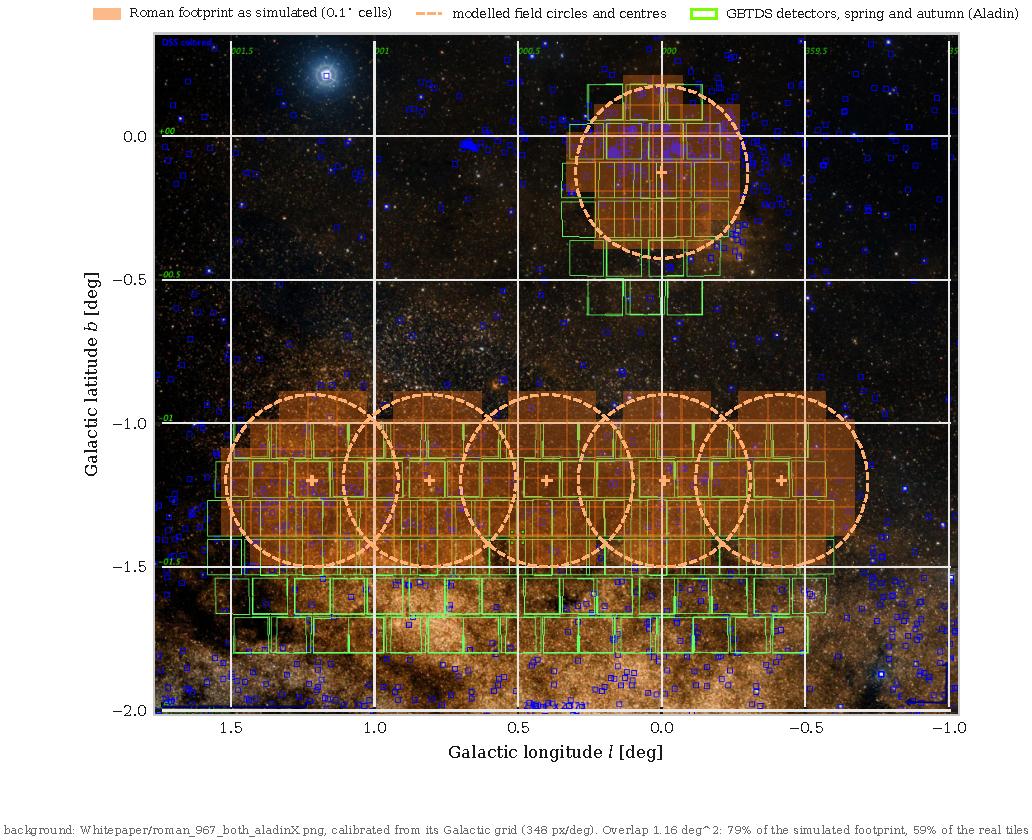
\includegraphics[width=\linewidth]{footprint_vs_gbtds}
\credit{background: \ads{2000A\%26AS..143...33B}{Aladin} (CDS), DSS images}
\end{column}
\begin{column}{.40\linewidth}
\small
\begin{itemize}
  \item $1{,}829$ sightlines over $68$\,deg$^2$: a Rubin exposure that contains part of a Roman field reaches $3.5^\circ$ beyond it
  \item $0.1^\circ$ grid inside Roman's fields ($147$ sightlines), $0.2^\circ$ outside; each carries its area
  \item Roman as simulated (orange): six circles, $1.47$\,deg$^2$, $\sim\!0.2^\circ$ closer to the plane than the adopted
        layout (green)
  \item The adopted detector geometry motivates a new footprint calculation
\end{itemize}
\end{column}
\end{columns}
\end{frame}

\begin{frame}{Backup: from the simulated sample to the sky}
\begin{itemize}
  \item The Monte Carlo does not draw events in proportion to the event rate: the lens mass and velocity draws miss a
        factor $\sqrt{\Ml}\,v_t$
  \item Each event therefore carries a weight $W\propto$ its event rate; every pooled fraction or median is weighted
  \item The weight costs precision; it is quoted as the Kish effective sample size
  \[
    \Neff = \frac{\left(\sum W\right)^2}{\sum W^2}
  \]
        e.g.\ $12{,}461$ simulated footprint detections weigh as $\Neff\approx4{,}000$
  \item Populations are never pooled: the weight contains $\sqrt{M}$ of the population drawn
  \item Yields: the weighted sample normalised to an expected number of events, $N(F)=F\,N_1$
  \item \textbf{Check:} mean event timescale in the comparison sightlines is $23.5$\,d, versus $23.8$\,d from OGLE-IV
\end{itemize}
\vfill
\refnote{\ads{2019ApJS..244...29M}{Mr\'oz et al.\ 2019, ApJS 244, 29}}
\end{frame}

\begin{frame}{Backup: the dust near the Galactic plane}
\begin{itemize}
  \item A declination rule assigned almost all model Roman sightlines to Bayestar. Within
        $\sim\!1^\circ$ of the plane it gives \textbf{3--6 times too little} extinction, measured against the VVV
        reddening map
  \item After reweighting outcomes against dust checked with VVV:
  \begin{itemize}
    \item Roman's yields $-33$ to $-38\%$ (its $10\%$ masses $-46$ to $-57\%$); Rubin's $-54$ to $-71\%$
    \item Roman retains the stronger precision within its footprint
    \item Roman's detection rate becomes $(23\pm5)\%$ below Penny et al.\ for the same $u_0$ range
  \end{itemize}
  \item \textbf{Dust-model update.} Rebuild the extinction tables from DECaPS, with near-infrared dust where DECaPS saturates;
        check against VVV before any run
\end{itemize}
\vfill
\refnote{\ads{2019ApJ...887...93G}{Green et al.\ 2019};
\ads{2025ApJ...992...39Z}{Zucker et al.\ 2025};
\ads{2020A\%26A...644A.140S}{Surot et al.\ 2020};
\ads{2006A\%26A...453..635M}{Marshall et al.\ 2006};
\ads{2019ApJS..241....3P}{Penny et al.\ 2019}}
\end{frame}

\begin{frame}{Backup: comparison with Sajadian \& Sahu (2023)}
This simulation builds on the paper's approach (separate photometric and astrometric Fisher matrices). With its mass
function ($dN/dM\propto M^{-1}$) and on its sample ($u_0<1$, peak inside the mission):
\vspace{2mm}
\begin{center}
\renewcommand{\arraystretch}{1.15}
\begin{tabular}{lcccc}
\toprule
\% to $10\%$ & $\tE$ & $\piE$ & $\tetE$ & $\Ml$ \\
\midrule
Sajadian \& Sahu 2023 & $67.0$ & $30.0$ & $99.2$ & $29.8$ \\
this work, rate-weighted & $67.4$ & $23.5$ & $75.5$ & $21.1$ \\
this work, per simulated event & $71.9$ & $42.1$ & $80.2$ & $38.1$ \\
\bottomrule
\end{tabular}
\end{center}
\begin{itemize}\small
  \item The weighted $\tE$ share is close. The published $\piE$ and mass shares lie between the two counting conventions shown here.
  \item $\tetE$ differs. The analyses use different astrometric noise models and treat parallax differently in the centroid fit.
\end{itemize}
\vfill
\refnote{\ads{2023AJ....165...96S}{Sajadian \& Sahu 2023}. The weighted comparison has $\Neff=1{,}472$. Detection cuts also differ.}
\end{frame}

\begin{frame}{Backup: a distant black hole}
\begin{columns}[T]
\begin{column}{.66\linewidth}
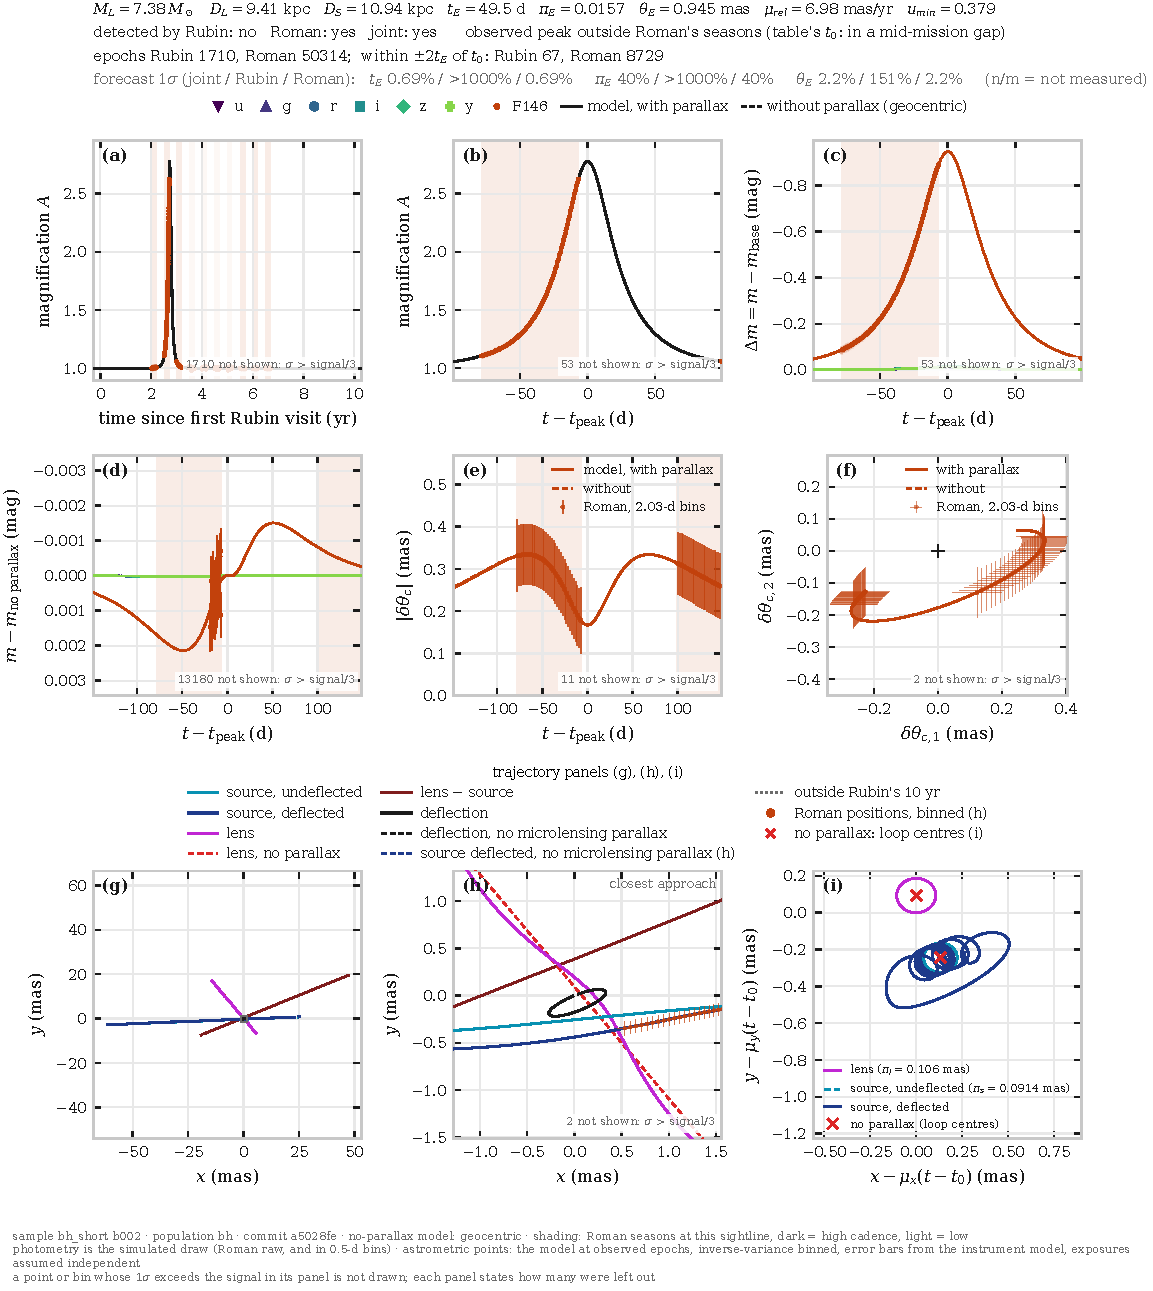
\includegraphics[width=\linewidth, trim=0 255 0 0, clip]{bh_short_b002_3x3}
\end{column}
\begin{column}{.32\linewidth}
\small
\textbf{$7.4\,\Msun$ at $9.4$\,kpc}, behind the Galactic centre; $\tE=50$\,d
\begin{itemize}
  \item Roman alone: $\tE$ to $0.7\%$, $\tetE$ to $2.2\%$
  \item but $\piE$ is tiny: \textbf{mass only to $\sim\!40\%$}
  \item Rubin does not detect it
\end{itemize}
The parallax limit in one event.
\end{column}
\end{columns}
\vfill
\refnote{September sample gallery, event bh\_short\_b002.}
\end{frame}

\begin{frame}{Backup: resolving the images --- the criterion}
\begin{itemize}
  \item At every visit: (i) both images detectable on their own (between saturation and the single-visit depth; blended
        light not added back); (ii) $\Delta\theta=\tetE\sqrt{u^2+4}$ above a bar
  \item Resolvable: $\ge3$ such visits
  \item Bars: $\mathcal{D}\sigma_{\rm ast}$ with $\mathcal{D}\approx5$ (detection limit) to $\approx20$ (S/N $\sim100$),
        built for Rubin's seeing-limited images; the PSF width ($105$\,mas for Roman, $\approx1''$ for Rubin)
  \item On Roman's $1.1$\,mas floor, $\mathcal{D}=5$ means separating sources $5.5$\,mas apart --- a twentieth of its PSF
  \item Roman's depth taken as F146 $=25.5$ ($5\sigma$, single exposure)
\end{itemize}
\vspace{2mm}
\centering\small
\begin{tabular}{lccc}
\toprule
Roman (dust-corrected) [\%] & black holes & neutron stars & ordinary \\
\midrule
$\mathcal{D}=5$ & $34$ & $1.7$ & $0.8$ \\
$\mathcal{D}=20$ & $15$ & $0.02$ & $\approx0$ \\
PSF & $0.25$ & $\approx0$ & $0$ \\
\bottomrule
\end{tabular}
\vfill
\refnote{\ads{2026ApJ..1009..116S}{Sajadian \& Makler 2026, ApJ 1009, 116}}
\end{frame}

\begin{frame}{Backup: how sensitive are the first results?}
\centering
\footnotesize
\renewcommand{\arraystretch}{1.12}
\begin{tabular}{p{.50\linewidth}p{.12\linewidth}p{.28\linewidth}}
\toprule
result & confidence & main risk \\
\midrule
For shared events, median timescale gain from Rubin is $<0.4\%$ & high & Roman photometric noise \\
Roman turns Rubin's detections into measurements & high & noise; astrometric floor \\
$\sim\!60\%$ of ordinary-lens detections are outside Roman's fields & high & latitude gradient \\
gap filling: only deep in gaps, short events & medium & small $\Neff$; not dust-corrected \\
negligible median satellite-parallax gain for black holes & high & September orbit model \\
black-hole $\tetE$ & high & --- \\
ordinary and neutron-star $\tetE$ and masses & medium--low & correlated astrometric floor \\
absolute yields $N_1$ & medium--low & dust near the plane \\
yields $N(F)$ & low & $F$ unknown to $\times6$ \\
image resolution & low & the criterion for Roman \\
\bottomrule
\end{tabular}
\end{frame}

\begin{frame}{Backup: Roman's adopted field layout}
\centering
\vspace{2mm}
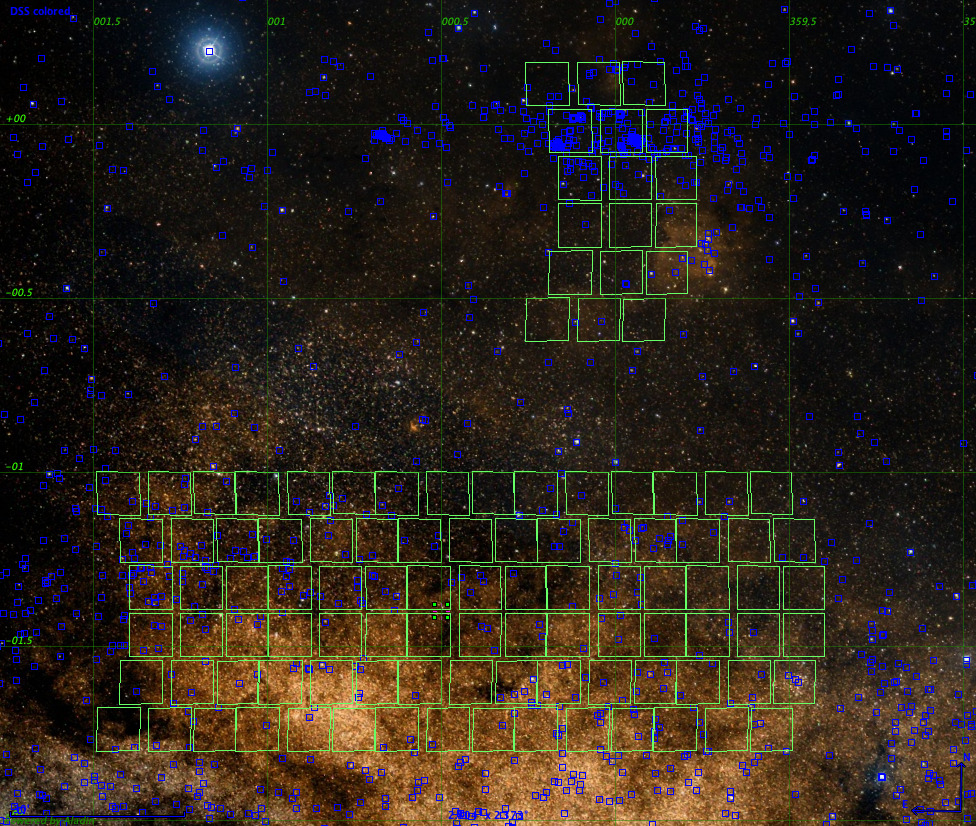
\includegraphics[width=.42\linewidth]{roman_gbtds_fields_spring}\hspace{6mm}%
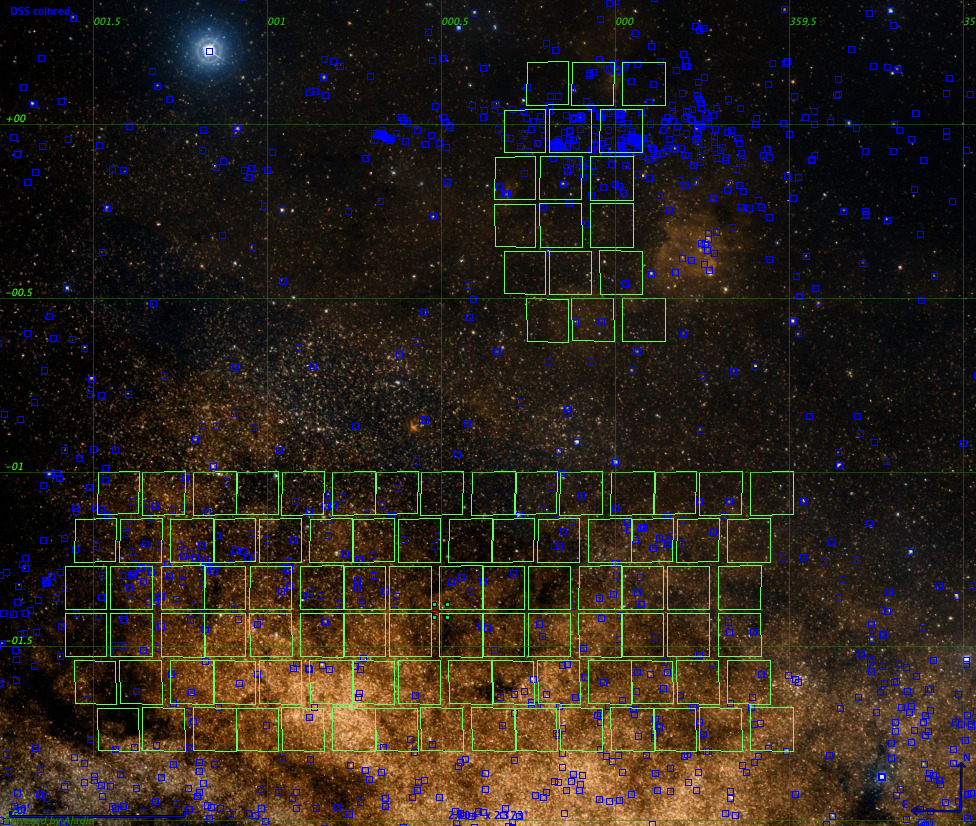
\includegraphics[width=.42\linewidth]{roman_gbtds_fields_autumn}\\[1mm]
\credit{\href{https://roman-docs.stsci.edu/roman-community-defined-surveys/galactic-bulge-time-domain-survey}{STScI, Roman GBTDS}}\\[2pt]
\small WFI detectors in the six GBTDS fields, spring (left) and autumn (right) seasons; the roll angle differs between them.
\end{frame}

\begin{frame}{Backup: forecasts in the literature}
\begin{columns}[T]
\begin{column}{.48\linewidth}
\centering
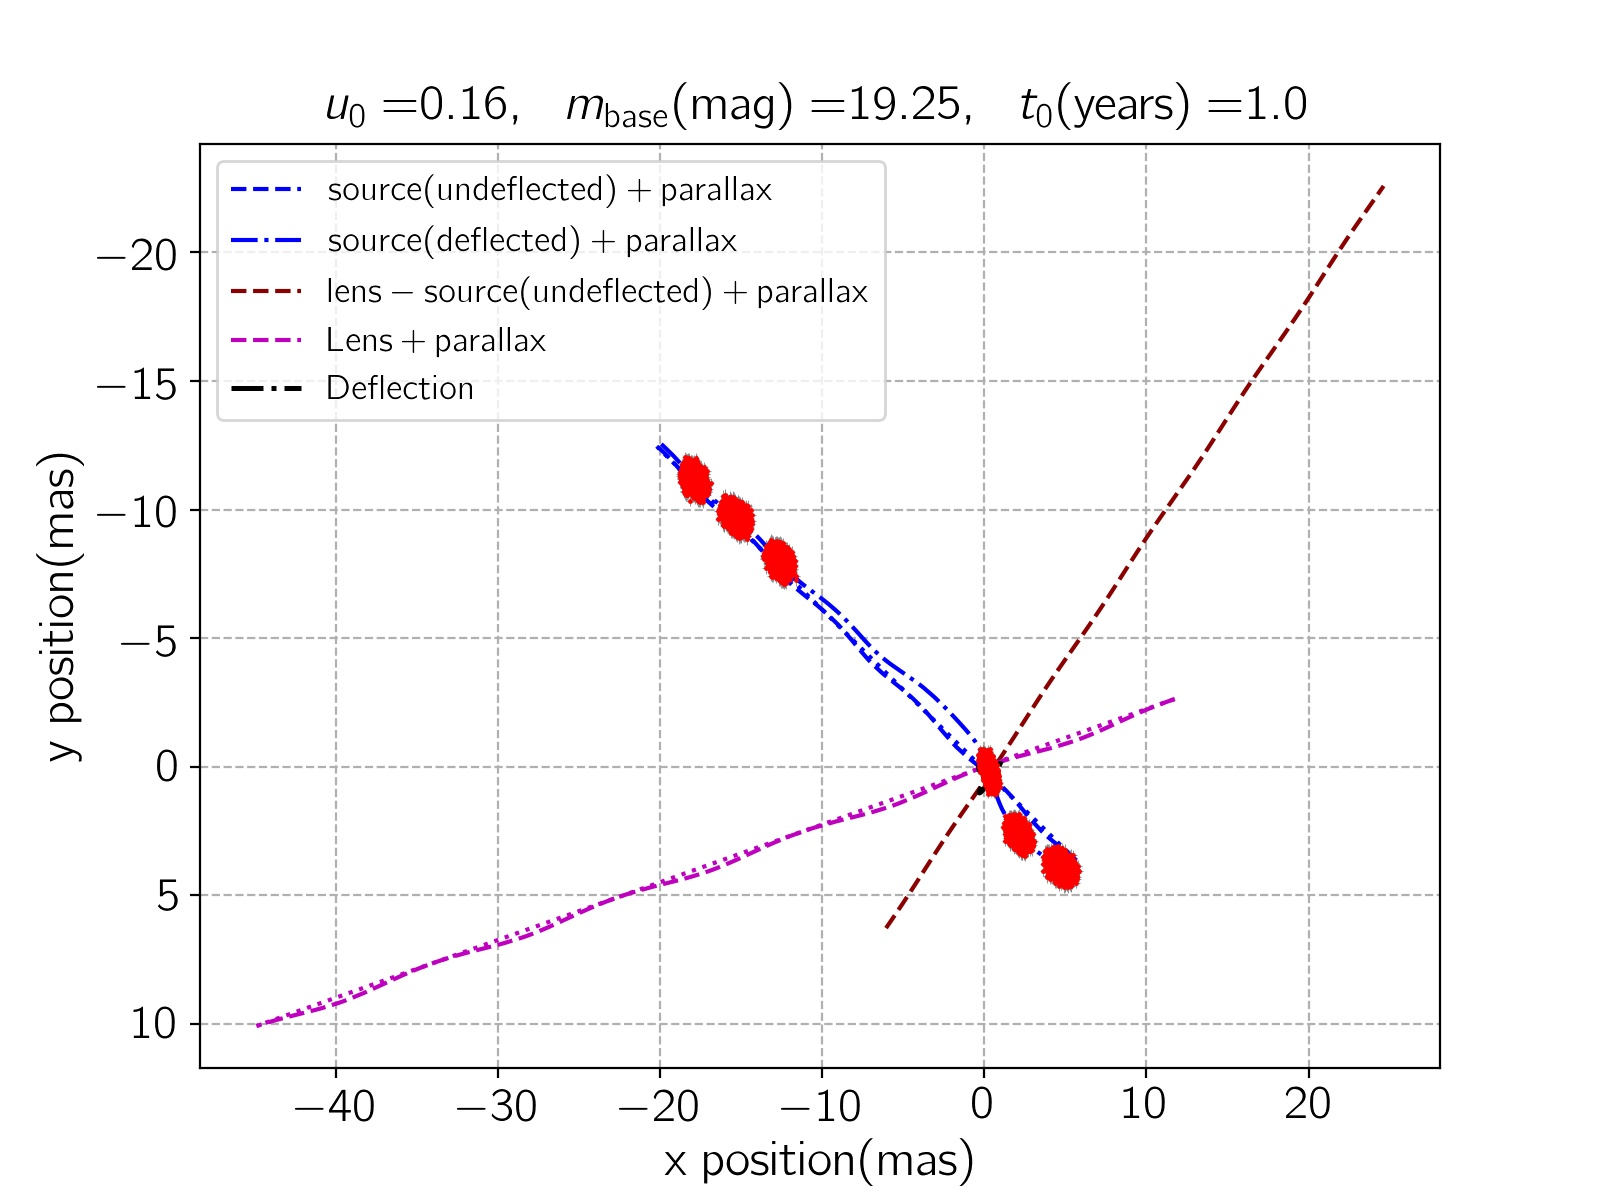
\includegraphics[width=.9\linewidth]{ss23_astrometry}
\credit{\ads{2023AJ....165...96S}{Sajadian \& Sahu 2023, AJ 165, 96}}\\
\footnotesize Roman: a simulated black-hole event, the source and lens tracks on the sky with the astrometric deflection.
\end{column}
\begin{column}{.48\linewidth}
\centering
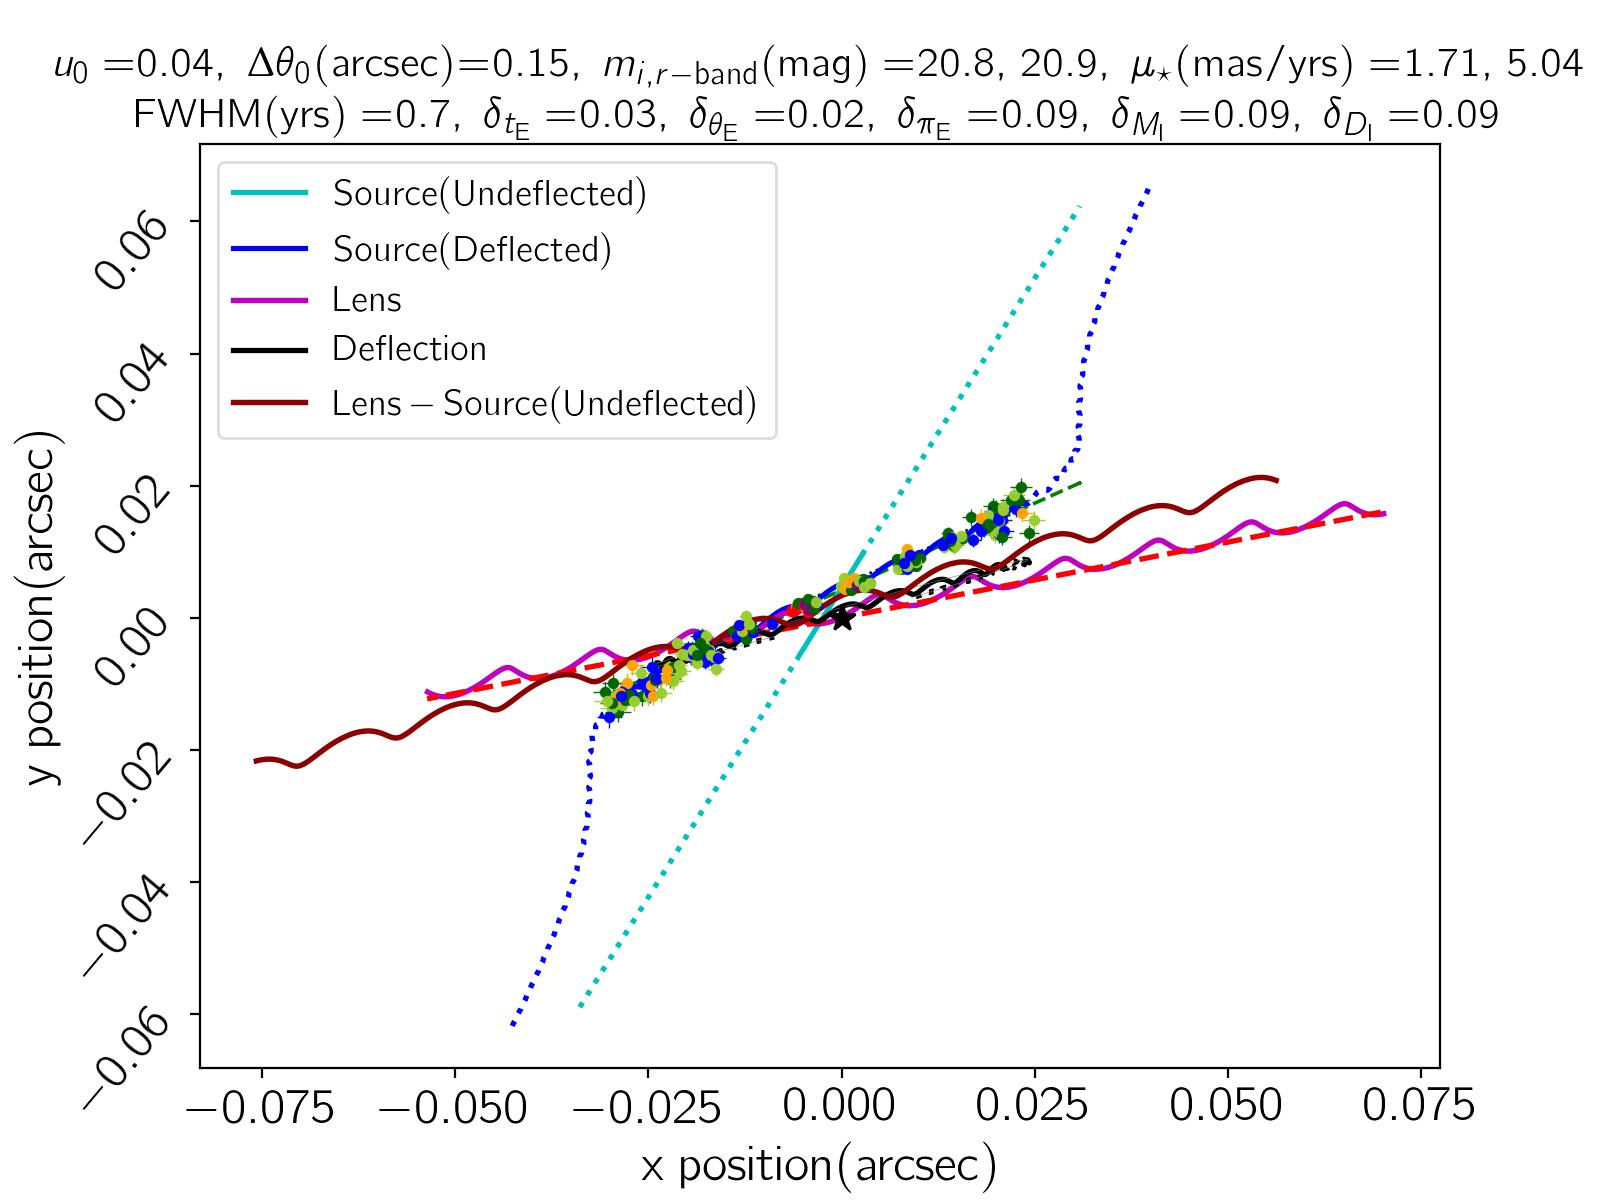
\includegraphics[width=.9\linewidth]{sm26_astrometry}
\credit{\ads{2026ApJ..1009..116S}{Sajadian \& Makler 2026, ApJ 1009, 116}}\\
\footnotesize Rubin toward the Large Magellanic Cloud: a $422\,\Msun$ simulated lens at $0.6$\,kpc, $\tE=5.4$\,yr, $\tetE=73$\,mas.
\end{column}
\end{columns}
\end{frame}

\end{document}
